%===============================================================================
% 
% emulateapj latex file for Mowgli paper
% 
% Started Naudus 2010-02-23
% 
% Notes:
%   - use \citep and \citet, and bibtex entries in references.bib
%     scrapeADS in scriptutils module (available via cvs form KIPAC) allows
%     you to generate these quickly from the ADS website.
%   - use auto newline in your editor to avoid very long lines - cvs merges
%     changes line by line.
%   - refer to the ApJ style guide for more details on including figures, 
%     equations, etc. 
% 
%===============================================================================

\documentclass[iop]{emulateapj}


% LaTeX definitions and macros:
\def\hmpc{\,{h$^{-1}$\,Mpc}}
\def\msun{M_{\odot}}
\def\hmsun{{\rm h}^{-1}\msun}
\def\sqdeg{{\rm deg}^{2}}
\def\kms{{\rm km s}^{-1}}

\def\ltsima{\; \buildrel < \over \sim \;}
\def\lsim{\lower.5ex\hbox{\ltsima}}
\def\gtsima{\; \buildrel > \over \sim \;}
\def\gsim{\lower.5ex\hbox{\gtsima}}
\def\eg{{\it e.g.}\,}
\def\ie{{\it i.e.}\,}

\def\zd{z_{\rm d}{ }}
\def\zs{z_{\rm s}{ }}
\def\re{r_{\rm e}{ }}
\def\sigmaSIE{\sigma_{\rm SIE}}
\def\Rein{R_{\rm Ein}}
\def\Reff{R_{\rm s,eff}}
\def\thein{\theta_{\rm Ein}}
\def\Dd{D_{\rm d}{ }}
\def\Dds{D_{\rm ds}{ }}
\def\Ds{D_{\rm s}{ }}

\def\xd{x_{\rm d}}
\def\yd{y_{\rm d}}
\def\qd{q_{\rm d}}
\def\phid{\phi_{\rm d}}
\def\xs{x_{\rm s}}
\def\ys{y_{\rm s}}
\def\qs{q_{\rm s}}
\def\phis{\phi_{\rm s}}

\def\pr{{\rm Pr}}
\def\pars{\mathbf{x}}
\def\parsi{x_i}
\def\data{\mathbf{d}}
\def\datai{d_i}
\def\datap{\mathbf{d}_{\rm p}(\pars)}
\def\datapi{d_{{\rm p},i}(\pars)}
\def\model{\mathsf{H}}
\def\modelA{\mathsf{H}_0}
\def\modelB{\mathsf{H}_1}
\def\chisq{\chi^2}
\def\rchisq{\hat{\chi}^2}

\shorttitle{Interactive lens modeling}
\shortauthors{Naudus et~al.}

\def\gmu{1}
\def\rutgers{2}
\def\kipac{3}
\def\oxford{4}
\def\mtsu{5}

\usepackage{amsmath,amssymb}
\usepackage{multirow}
\usepackage{float}
\usepackage{xspace}
\usepackage{longtable}
\usepackage{appendix}

% Macros:

\def\theapplet{{\sc Mowgli}\xspace}
% Manually-operated widget for gravitational lens identification

\def\xdi{x_{{\rm d},i}}
\def\ydi{y_{{\rm d},i}}
\def\phidi{\phi_{{\rm d},i}}
\def\qdi{q_{{\rm d},i}}
\def\Reini{R_{{\rm Ein},i}}
\def\alphai{\boldsymbol{\alpha}_{i}}
\def\Nd{N_{\rm d}}

\def\xsj{x_{{\rm s},j}}
\def\ysj{y_{{\rm s},j}}
\def\phisj{\phi_{{\rm s},j}}
\def\qsj{q_{{\rm s},j}}
\def\reffj{R_{{\rm eff},j}}
\def\Fsj{F_{{\rm s},j}}
\def\Ns{N_{\rm s}}

\def\TODO#1#2{{\bf TODO: {#1}: {#2}}}
\def\QUERY#1#2{{\bf QUESTION FOR {#1}: {#2}}}
\def\ACHTUNG#1#2{{\bf ATTENTION {#1}! {#2}}}
\def\NEW#1{{\bf{#1}}}

% ==============================================================================

\begin{document}

\title{\theapplet: Interactive Manual Modeling of Strong Gravitational Lenses}

\author{Philip~S.~Naudus\altaffilmark{\gmu,\rutgers}}
\author{Philip~J.~Marshall\altaffilmark{\kipac,\oxford}}
\author{John~F.~Wallin\altaffilmark{\gmu,\mtsu}}

\altaffiltext{\gmu}{Department of Computational and Data Science, George Mason University, Fairfax, VA 20030, USA} 
\altaffiltext{\rutgers}{Department of Physics \& Astronomy, Rutgers University, Piscataway, NJ 08854, USA} 
\altaffiltext{\kipac}{KIPAC, P.O.\ Box 20450, MS29, Stanford, CA 94309, USA} 
\altaffiltext{\oxford}{Department of Physics, University of Oxford, Keble Road, Oxford, OX1 3RH, UK} 
\altaffiltext{\mtsu}{Computational Science Program \& Department of Physics, Middle Tennessee State University, Fairfax, VA 20030, USA} 

% ------------------------------------------------------------------------------

\begin{abstract}

We present \theapplet, a web-based tool for modeling gravitational lens systems 
designed to be used by citizen scientists when analyzing candidates selected
from very large imaging surveys. 
%
The lens and source models are constructed manually, via a cursor-controlled
Java applet; multiple mass components, image masks and source brightness
distributions can be placed directly on an astronomical image of the lensing
system, and then manipulated. The predicted lensed and PSF-convolved images are
generated in real time, as are the caustics and critical curves of the lens
model.
%
The lens model comprises any number of elliptically-symmetric singular
isothermal mass distributions, while the sources are modeled as having
elliptically-symmetric Gaussian surface brightness distributions.
The model parameters are optimized manually by the user, with
reference to both a display of the image residuals and a quantified goodness of
fit statistic. An experienced user can typically find a reasonable model in a
few minutes, with refinements to improve the accuracy taking longer.
Automated optimization is also provided, to refine the approximate models
found by hand.
%
We demonstrate the applet's operation by modeling the twenty candidate lens
systems identified in the SDSS imaging survey as part of the CASSOWARY project.
We confirm, by modeling, 12 of the 20 systems are gravitational lenses,
6 are likely to be lenses, and 2 systems cannot be easily modeled as
gravitational lenses. We measure the physical Einstein radii of the CASSOWARY
lenses (at redshift 0.3--0.6) and find them to be comparable
(10--50~kpc) to those of group-scale lenses found at higher redshift in higher
resolution imaging surveys.

\end{abstract}

% Full list of options at http://www.journals.uchicago.edu/ApJ/instruct.key.html

\keywords{%
   gravitational lensing --- 
   methods: data analysis
}

% ------------------------------------------------------------------------------

\section{Introduction}
\label{sec:intro}

Strong gravitational lenses -- massive objects, such as galaxies or  clusters of
galaxies, that  cause multiple-imaging of objects lying directly behind them --
have a wide range of applications in astrophysics and cosmology \citep[see \eg
][for an introduction]{SKW06}. Notably, lenses have been used very successfully
in recent years to allow us to measure the distribution of dark and luminous
matter in galaxies  \citep[\eg][]{Gav++07,Koo++09}, groups
\citep[\eg][]{Lim++09}  and clusters \citep[\eg][]{Bra++06,Lim++08}, and to 
provide a magnified view of the high redshift universe
\citep[\eg][]{Pet++02,Sta++08,Swi++09}, including populations of galaxies not
easily studied by ordinary means  \citep[\eg][]{Bla++99,Sta++07,Bra++09}. 

Searches for gravitational lenses typically have two stages, namely the
selection of objects that could be lenses (``lens candidates''), and then the
verification (or rejection) of those candidates by follow-up observation.  There
is, inevitably, a trade-off between completeness and efficiency in the
candidate  selection stage. For example, in the CLASS survey, flat-spectrum 
radio sources were selected that appeared as extended, not point-like, objects
in the radio maps of the FIRST survey \citep{Bro++03}. Some 16,500 of these were
observed in a  VLA snapshot campaign and found to have gravitational lens image
morphologies, leading to a complete sample of 22 systems. In contrast, the SLACS
team selected just 141 luminous red galaxies from the SDSS spectroscopic survey
whose spectra showed clear evidence of there being a higher redshift emission
line galaxy in the same fiber aperture; HST snapshot  follow-up of these
revealed 85 of them to be certain galaxy-scale gravitational lenses
\citep{Bol++06,Aug++09}. 

A promising way to find useful gravitational lenses in greater numbers is to
search optical images directly. Sources are plentiful in the visible wavebands,
where faint blue galaxies appear on the sky at a density  of $\sim 100$ per
square arcminute \citep[\eg]{Ben++04}; these sources can in principle be
separated from the intervening lens galaxy light by their color and the image
morphology \citep[see \eg][]{Mou++07,Cab++07,Fau++08,Hen++08,Jac08,Mar++09}. 
Lens-finding in optical images has a long history, stretching back to the first
lensed quasar \citep{WCW79} and the first giant cluster arcs \citep{For87} --
they were discovered as soon as enough sky was surveyed at sufficient
resolution. This remains perhaps the most compelling reason to consider
lens-searching in this way: high resolution optical imaging surveys covering
very wide areas are being carried out and planned for the coming decade, with
very different primary science (such as weak lensing, supernova discovery,
galaxy photometric redshift surveys, asteroid tracking and so on) in mind.
Between them, the 
CFHTLS ($\sim 170 \sqdeg$), %\citep[$\sim170\sqdeg$][]{CFHTLS}, 
SDSS~I-III  ($\sim 10,000 \sqdeg$), %\citep[$\sim10,000\sqdeg$][]{SDSS}, 
PS1 ($\sim30,000 \sqdeg$), %\citep[$\sim30000\sqdeg$][]{PS1},
DES  ($\sim 5,000 \sqdeg$) %\citep[$\sim5000\sqdeg$][]{DES}, and
and LSST ($\sim20,000 \sqdeg$) %\citep[$\sim20000\sqdeg$][]{LSST}
aim to image the entire sky at sub-arcsecond image quality, revealing
many thousands of well-resolved multiple image 
systems~ \citep[see \eg][]{Ogu++10,LSSTScienceBook}.

One of the biggest challenges when exploiting these rich new datasets  to find
large numbers of new gravitational lenses will be increasing the efficiency of
the process.  Simple database selections based on object (either lens galaxy or
lensed image) color and morphology typically produce samples that are relatively
impure \citep{All++07,Hen++08,Fau++08}. In the case of {\it simple}  lenses,
efficiency can be increased by using filters specifically designed to catch the
most common characteristic lensed image geometries, albeit at the cost of some
completeness \citep{Mar++09,Kub++09}. The more simplistic the lens
identification algorithm, the less complete the sample of candidates will be;
moreover, it is the simple algorithms that are most likely to fail on the
complex lenses, which are of interest for at least some of the science
projects discussed above. 

Some automated methods do contain a crucial ingredient: a lens model. Indeed,
we follow \citet{Mar++09} and argue that a {\it necessary condition for an
object to be considered a good lens candidate  is that its system of images be
explained by a gravitational lens model}. Fitting the image data for a
candidate system by  computer modeling allows  objective and quantitative
statements to be made about whether or not the system is a gravitational lens
or not. However, the process is typically quite CPU-intensive, especially for
complex lenses \citep[see e.g.][for the state of the art]{Bre++10}. Also, the
data have to be carefully masked and the putative lens galaxy light subtracted
before the fit, to avoid the fitting algorithms becoming confused by unlensed
features in the image \citep[see \eg][]{Bol++06}.  Indeed, fully automated
lens identification has not yet been demonstrated for complex lenses.

The model fit condition has, effectively, been applied in all imaging survey
lens searches carried out to date,  including those based purely on visual
inspection of the pre-selected candidates \citep[\eg][]{Mou++07,Jac08}. In
these searches, an expert inspector carried out a qualitative  {\it mental
modeling} of the image data associated with each candidate, including
accounting for features in the image that are {\it not} due to lensing.
\NEW{The presentation of the image data is very important. Informative color
composites can be more readily assessed by an inspector than can  a single
filter image: both the color scale and the image stretch will likely have been
chosen to maximize the visibility of the features of interest in the image.
Moreover, such images are usually stored in compressed JPEG  format, reducing
the data storage and transfer overheads.} Mental modeling is fast because it
uses the inspector's  own powerful neural network to classify objects based on
a (typically) large training set of previously experienced lenses and
non-lenses.  However, it is labor-intensive -- and so may lead to
incompleteness and poorly-defined selection functions as inspector fatigue
sets in. One solution to this problem is to have many inspectors classify the
same sample. Another issue is the reliability of the human classification: are
mental models really good enough? If the training set is not large or diverse
enough, omissions and mis-identifications will occur. This problem is solved
by actually fitting the data, to show that the observed features are
consistent with being multiple images of the same source, distorted by a
plausible gravitational  lens in a plausible way.  

In this work, we explore a hybrid approach between computer and mental lens
modeling. We introduce and demonstrate a new  tool,
\theapplet,\footnote[1]{\theapplet is an acronym, for Manually Operated Widget
for Gravitational Lens Identification.}  for interactively fitting images of
candidate gravitational lenses. This web-based Java applet should allow large
numbers of lens inspectors, with minimal training, to classify candidate
complex  lenses by making quantitative {\it manual models} of them. \NEW{As a
first step towards this goal, we ask here the following questions: Can
approximate lens models be made in a usefully short time, using survey imaging
data? How do the estimated lens model parameters and their uncertainties
differ when color JPEG ``data'' are used, instead of single filter FITS images?
From models inferred using \theapplet, what can we conclude about the
CASSOWARY lens candidates?}

This paper is organised as follows. We first set the scene in
Section~\ref{sec:citsci}, briefly describing the   online citizen science
community, making a case for extending  their activities to
appropriately-supported detailed data modeling. In Section~\ref{sec:model}, we
describe our particular data model, including the gravitational lens itself, but
also how we treat the input data. We then describe, in
Section~\ref{sec:explore},  how the parameters of this model are manually 
optimized, presenting the  \theapplet applet.  In Section~\ref{sec:sample}, we
define our demonstration dataset, the CASSOWARY candidate lens sample, and in 
Section~\ref{sec:results} present our results from manually modeling these
systems. We discuss our findings and implications for future work in 
Section~\ref{sec:discuss} and draw conclusions in  Section~\ref{sec:concl}.


% ----------------------------------------------------------------------------

\section{Lens Modeling by Citizen Scientists}
\label{sec:citsci}

One way of solving the problems of visual lens-searching is to
``crowd-source'' them to a large group of volunteer ``citizen scientists.''
One of the largest and most successful of these projects in astronomy is the
Zooniverse,\footnote{\texttt{http://zooniverse.org}} perhaps best known for
its initial project, Galaxy Zoo. The initial premise of this project was that
people, even those with no astronomical training, are better than computers at
classifying the morphology of galaxies. In the 3 years  since its launch in
2007, more than 250,000 Zoo users classified galaxies; in a single year,
participants generated over 60 million classifications \citep{gz1}. More
recently, citizen scientists on this site have been involved in detecting
solar storms, characterization of lunar terrain, and modeling interacting
galaxies. The users of the Zooniverse are members of the public who are
motivated by participation in the scientific enterprise and are capable of
certain kinds of expert analyses following some training \citep{Rad++2010}.

Encouraged by the successes of Galaxy Zoo \citep[\eg][]{gz1,gz2,gz3}, we propose
that lens identification is a task that can be performed by citizen scientists.
In this paper, we describe a way of providing citizen scientists with this
training, enabling them to identify gravitational lenses through image modeling.
Rather than their  absorbing various treatises on lensing theory and the
literature on the various lensing effects, we suggest that it is more important
that users learn what gravitational lensing {\it looks like}, and that this
learning is best done by {\it playing} with an {\it interactive lensed image
modeler}. Moreover, the results of the users' attempts to manually model
candidate lenses will contain information about the likelihood of their actually
being lenses, allowing the systems to be ranked and rejected. We do not test
these suppositions rigorously here, but merely take the first step towards a
crowd-sourced gravitational lens search by presenting a tool, ``\theapplet,''
for manually modeling images of gravitational lenses, and demonstrate its use on
twenty candidate systems from the SDSS imaging survey, selected by the CASSOWARY
project~\citep{Bel++07,Bel++09}. 

Moreover,  we anticipate that \theapplet, which we make available as a web-based
Java applet, will also be of use to those in the professional astronomy
community working with gravitational lenses. Being able to make a quick model of
a gravitational lens is not only useful for assessing its very plausibility; it
is also a useful first step in planning further investigations (for example,
follow-up spectroscopy of the lensed galaxies), or to find a suitable starting
point for a more detailed analysis. The likelihood function associated with
complex strong lens image data is not easy to explore; it typically has multiple
peaks, with very steep gradients and high skewness. The experience is that the
most difficult part of the inference problem is getting close to the global
peak; once there, simple optimizers or Markov Chain Monte-Carlo  samplers can
characterize that peak well, but the majority of the CPU time spent by these
automated routines is typically in the initial peak-finding stage. 
Sophisticated, but time-consuming, sampling techniques are required  to solve
this problem \citep{Bre++10}.  A human operator can navigate the likelihood
function more efficiently, using their experience to recognize the various
patterns in the residuals and not being thrown off by temporarily terrible
goodness of fit; indeed, cluster strong lens modeling often involves some
skilled manual parameter optimization, with conjugate images being identified by
trial and  error~\citep[\eg][]{Kne++93,Smi++01}.  As part of our demonstration
then, we use \theapplet to measure the parameters of the CASSOWARY lenses, and
predict the total magnifications they provide.

Although there have been a number of on-line Citizen Science projects, most have
focused on the analysis of large data sets.   Projects such as  Moon Zoo, Galaxy
Zoo, and Stardust allowed volunteers to look for anomalies in large sets of
images.   To date, however, there have been very few Citizen Science projects
that engage volunteers in modeling complex systems. One such project in
astronomy is the Cosmic Mergers \citep{Hol++10,Wal++10};
here, the primary challenge in helping volunteers with  little training model
complex systems is to develop an intuitive interface to the modeling
``engine.''    A secondary challenge is developing ways of combining the results
from many volunteers into a better understanding of the parameter space near
regions that are close matches to the desired data.    Although we have created
an intuitive interface suitable for lens identification  volunteers, we will not
be addressing the second issue of results synthesis in this paper.  Instead, we
focus on the engine and its interface itself, which we describe in the next two
sections. 


% ----------------------------------------------------------------------------

\section{Gravitational Lens Model}
\label{sec:model}

In this section we describe our mathematical model for complex lenses, and the
likelihood function of the multi-filter imaging data. This constitutes the inner
workings of \theapplet, whose user operation is described in
Section~\ref{sec:explore} below. The lens and source model components are
similar to those used by \eg \citet{Mar++07} and \citet{Bre++10},  as is the
image prediction and likelihood function. In several key places, our approach
differs from this previous work, and we point these out explicitly as we go.

%  -  -  -  -  -  -  -  -  -  -  -  -  -  -  -  -  -  -  -  -  -  -  -  -  -  

\subsection{Lens mass model}

We assume that complex gravitational lenses can be well-approximated by a set
of $\Nd$ simple components, whose gravitational potentials can be simply
summed. We imagine that each lens galaxy in the field (usually recognizable as
an elliptical galaxy of old, ``red'' stars) has an elliptically-symmetric,
centrally concentrated mass distribution associated with it, and that this
mass distribution is a mix of stellar matter, and dark matter, which  extends
to higher radii than the stars.  The resulting total density profile is found,
in isolated galaxies, to be well approximated by a simple power law of
index~$-2$  \citep[see \eg][]{Koo++03}. We therefore take each lens component
to be one of these ``singular isothermal ellipsoid'' (SIE) models. The dark
matter need not just be associated with the visible light, and we do not, in
fact, enforce this: our mass components are free to be positioned anywhere in
the field. However, even in groups and clusters, it is usually the case that
the overall dark matter halo (required by the observable lensing effects) is
centered on one of the galaxies in the cluster \citep[see \eg][ for an extreme
example]{Bra++06}. 

Each lens mass component (which we index here with $i$ from 1 to $\Nd$) has 5
parameters associated with it: its position $(\xdi,\ydi)$, the axis ratio of
the elliptical isodensity contours $\qdi$, orientation angle $\phidi$
(measured from the $x$-axis to the major axis of each ellipse), and Einstein
radius $\Reini$ (in arcsec). The Einstein radius of a mass component is
(approximately) where an Einstein ring would form, if that component was an
isolated galaxy -- in practice, the nearby mass components will contribute
their own  lensing effects and the images will not appear at $\Reini$ from the
mass component. Since we do not (in general) know the redshifts of the lens
and the source, we cannot use the total mass of the component as a parameter:
the Einstein radius is the best we can do to describe the lens ``strength'' of
each component in the model.

The angle though which passing light rays would be deflected by each component,
$\alphai$, can be calculated following \citet{KSB94}.  This deflection angle
varies over the field of view -- and indeed must be calculated for each pixel of
the image. $\alphai$ is just the spatial derivative of the lens potential, so
the deflection angles for each component can be computed and simply summed
together to get the overall deflection caused by the lens. Likewise, the
convergence and shear fields for each component (the second derivatives of the
lens potential) can be simply summed, and then combined to compute the
magnification of the lens at each point in the image. Although the magnification
is infinite on the critical curve, it is not computationally feasible to handle
infinitely large values. For this reason, the critical curve is determined by
finding the contour along which the magnification exceeds a predetermined
threshold. The magnification and deflection fields could be mapped in more
detail by computing them at intervals of a fraction of a pixel \citep[as
in][]{Mar++07}; we trade accuracy for computation speed at this point, and work
with the smallest grids possible. 


%  -  -  -  -  -  -  -  -  -  -  -  -  -  -  -  -  -  -  -  -  -  -  -  -  -  

\subsection{Lensed Image Prediction}
\label{sec:model:image}

A light ray arriving from a position $\boldsymbol{\theta} = (\theta_x,\theta_y)$
on the sky was actually emitted from a position  $\boldsymbol{\beta} =
(\beta_x,\beta_y)$, but has been deflected through $\boldsymbol{\alpha}$: to
predict the image of a lensed source, we calculate  $\boldsymbol{\beta}$ for
every pixel in the image using the lens equation,
\begin{equation}
  \boldsymbol{\beta} = \boldsymbol{\theta} - 
                         \boldsymbol{\alpha}(\boldsymbol{\theta}),
\end{equation}
and then look up the value of the surface brightness $I(\boldsymbol{\beta})$  of
the background source galaxy at that  position~\citep[\eg][]{New++02,Mar++07}.  
In practice, we do not  {\it know} what the deflection angle 
$\boldsymbol{\alpha}(\boldsymbol{\theta})$ is, nor do we {\it know} what the
source galaxy looks like: all we can do is assume a model for the lens and a
model for the source, and compare the resulting predicted images with what we
actually see -- and then vary the parameters of our model to improve the match.

We model the source galaxy as an elliptically-symmetric blob with Gaussian
profile. This is a reasonable approximation for the ubiquitous compact faint
blue galaxies seen in, for example, the Hubble Deep Field: these galaxies are
the most likely sources since they are the most common background objects. In
the cases where the source is more complex than this, or if more than one source
is required to match the observed system of gravitational arcs, we allow for
multiple Gaussian source components. Each of these $\Ns$ sources has 6
parameters: its position $(\xsj,\ysj)$, ellipse axis ratio $\qsj$, orientation
angle $\phisj$ (the angle measured in radians from the positive $x$-axis
counter-clockwise to the major axis of the ellipse),  its total brightness
$\Fsj$, and its half-light radius $\reffj$ in arcsec (within which half the
total brightness of the galaxy is contained). The total brightness of the
unlensed galaxy is the easiest parameter to determine -- we describe two ways in
which we do this in Section~\ref{sec:chiSq} below.

%----------------------------------------------------------------------------

\section{Data}
\label{sec:data}

\NEW{\theapplet is designed to work with images uploaded in one of two
formats, JPEG and FITS. Color JPEGs are highly informative to a human inspector,
with the contrast between different types of galaxy made clear by the different
hues present, and the JPEG compression acting to suppress noise in the dark
background areas. However, the noise properties (pixel value uncertainties)
of such images are not representative of the original raw data, which is
usually stored in single filter, FITS format data files. In this section we
outline the various considerations necessary when working with the candidate 
image data in general, and JPEG and raw FITS date in particular.}

\NEW{The example lens systems we consider in this paper come from the SDSS
survey,\footnote{\texttt{http://skyserver.sdss.org/public/en/tools/chart/navi.asp}}
a ready source of astronomical FITS image data with corresponding JPEG
visualisations. However, \theapplet can work with image data from any
telescope.}

% -  -  -  -  -  -  -  -  -  -  -  -  -  -  -  -  -  -  -  -  -  -  -  -  -  

\subsection{Masking}
\label{sec:masking}

In every astronomical image, there will be artifacts which are not present
in the predicted image, such as the lens galaxy and background. \theapplet
allows the user to place masks over these pixels in order that they do not
count toward the error between the predicted and astronomical images.
Masked pixels are ignored when computing the goodness of fit (Section
\ref{sec:chiSq}).

In order to aid the user in masking out background pixels, \theapplet allows
the user to import a ``masking image.'' If the masking image is not grayscale,
\theapplet will convert it to grayscale after importing it. The user is then
able to set a threshold-- pixels located at the pixels of the masking image
which fall below the threshold are masked.

In the models presented in this paper, the SDSS JPEG image mask was used for
for both the JPEG and FITS models, in order that the same
pixels were masked in both sets of models. In general, each user would
make their own mask for their uploaded image.

%  -  -  -  -  -  -  -  -  -  -  -  -  -  -  -  -  -  -  -  -  -  -  -  -  -  

\subsection{PSF Blurring}
\label{sec:psf}

The images predicted by the lensing of our model source components by our model
complex lens are those that would be seen by a perfect telescope above the
Earth's atmosphere. We need a predicted image that we can compare to our noisy,
blurry data -- and so we convolve the images described in the previous section
by a circularly symmetric Gaussian point spread function (PSF) to approximate
the blurring effect of the atmosphere and telescope optics.

For speed, we map this model PSF onto a small pixel grid ($\gtsima$ 2 full PSF 
widths across) and perform the convolution integral numerically.  The size of
this pixel grid depends on the observed image we are working with. For example,
a typical resampled  SDSS image might have pixels that are 0.3'' wide and a PSF
of FWHM 1.4''  ($\simeq 5$ pixels); the  model PSF would then have Gaussian
width 0.6'' and  we would map the model PSF on to a $11 \times 11$~pixel grid.
This choice was optimised for computation speed. 

If the user imports a FITS image and the PSFWID header keyword exists, the PSF
is set to the value in the header. For SDSS FITS images, PSFWID is the FWHM
of the PSF in arcseconds, as determined using a double-Gaussian fit. If the
user imports a JPEG image or a FITS image without the PSFWID header, the PSF
defaults to 1.4''. The PSF FWHM may be edited by the user at any time.


%  -  -  -  -  -  -  -  -  -  -  -  -  -  -  -  -  -  -  -  -  -  -  -  -  -  

\subsection{Measuring goodness of fit}
\label{sec:chiSq}

\NEW{Raw image data stored in FITS files have well-understood error
properties, allowing us to use correspondingly well-motivated goodness of fit
statistics when comparing predicted and observed images. In contrast, the
pixel values of a color JPEG are rarely proportional to the astronomical flux
received, and the JPEG creation process involves some image smoothing and
compression. (This is why we refer to the source's ``brightness,'' rather than
its ``flux,'' in Section~\ref{sec:model:image} above.) Nevertheless, it is
possible to define a statistic to quantify goodness of fit on a  {\em
relative} scale. In this section we define the statistics we use to quantify
goodness of fit for both JPEG and raw FITS data.}

Typically, raw optical astronomical images have pixel values with
Gaussian-distributed  errors, which motivates the use of the $\chi^2$ statistic
as a measure of goodness of fit. We defined the $\chi^2$ of the models fitted
to FITS images using:
\begin{equation}
  \chi^2 = \sum_i \frac{\left( F_{\text{obs},i} - F_{\text{pred},i} \right)^2}
                          {\sigma_i^2},
  \label{eq:rchisq}
\end{equation}
where the $\sigma_i$ used was the same for all pixels, and determined by
computing the standard deviation of the background pixels. 
These background pixels were determined by applying a simple brightness 
threshold to the masked pixels.

We are unable to use this same statistic in order to determine the error
associated with models fitted to color JPEG images, because we cannot estimate
the noise in the image in the same way.   In  JPEG-filtered images, much of
the original background noise is smoothed away. This leads to an artificially
small mean square residual  pixel value. Moreover, any remaining background is
likely to be quite different in each filter.  Given the unknown, and difficult
to estimate, pixel error,  we are prevented from estimating a meaningful 
absolute goodness of fit. Instead, we define a simple  relative statistic
$\rchisq$ for each channel:
\begin{equation}
  \rchisq = \frac{\sum_i \left( F_{\text{obs},i} - F_{\text{pred},i} \right)^2}
                          {\sum_i F_{\text{obs},i}^2}.
  \label{eq:rchisq}
\end{equation}
This quantity compares the mean squared pixel value in the residual image  with
the  mean squared pixel value in the data image: if $\rchisq = 0.05$, then the
model has accounted for 95\% of the features in the image.
We then use the average of $\rchisq$ over the red, green and blue image 
channels:
\begin{equation}
	\rchisq_\text{tot} = \frac{1}{3}\sum_j \rchisq_j.
  \label{eq:omega}
\end{equation}
%We take the average
%of this $\rchisq$ value over the three channels, and subtract from one  to get a
%final goodness of fit statistic~$\Omega$, which is best  thought of as the
%``explained feature percentage:''
%\begin{equation}
%  \Omega = \left( 1 - \frac{1}{3}\sum_j \rchisq_j \right) \times 100\%.
%  \label{eq:omega}
%\end{equation}
%Here, the index $j$ runs over the three channels of the image. This quantity
%should have a value approaching 100\% for a very good fit,  0\% for a null
%model, and be negative for bad fits (where features are predicted but not
%observed in some places, and observed but not  predicted in others).

\NEW{We compute parameter uncertainties  by varying each parameter separately
until, for FITS images,  the $\chi^2$ value increases by $\delta_\text{FITS} =
1$. The quoted uncertainties are symmetrized, by exploring $\chi^2$ in both 
directions and averaging the two results. If a parameter is increased
significantly without a significant change in $\chi^2$, the uncertainty of the
parameter is assumed to be infinite. For instance, if the ellipticity of a
source is small, varying the rotation will result in little to no change of
the modeled arcs, resulting in an infinite uncertainty in the rotation.}

\NEW{We note that $\delta_\text{FITS}$ will not, in general,  be equal to
$\delta_\text{JPEG}$ for JPEG images, due to the significant differences
between JPEG and FITS images. In Section~\ref{sec:results:JPEGvsFITS} below,
we calibrate the JPEG-fitted parameter  uncertainties against the FITS-fitted
parameter uncertainties, for the CASSOWARY sample SDSS data, finding an
approximately linear relationship between them}.


% ----------------------------------------------------------------------------

\section{Parameter Space Exploration}
\label{sec:explore}

The data model described in the previous section can be thought of as a black
box, taking a list of model parameter values as input and producing a
predicted image and its associated chi-squared value as output. The next task
is to optimize this model, varying the parameters to decrease the value of the
chi-squared misfit statistic and (ultimately) find the best-fitting models. 

%%%%%%%%%%%%%%%%%%%%%%%%%%%%%%%%%%%%%%%%%%
\addtocounter{figure}{-1}
\begin{figure*}[!ht]
\centering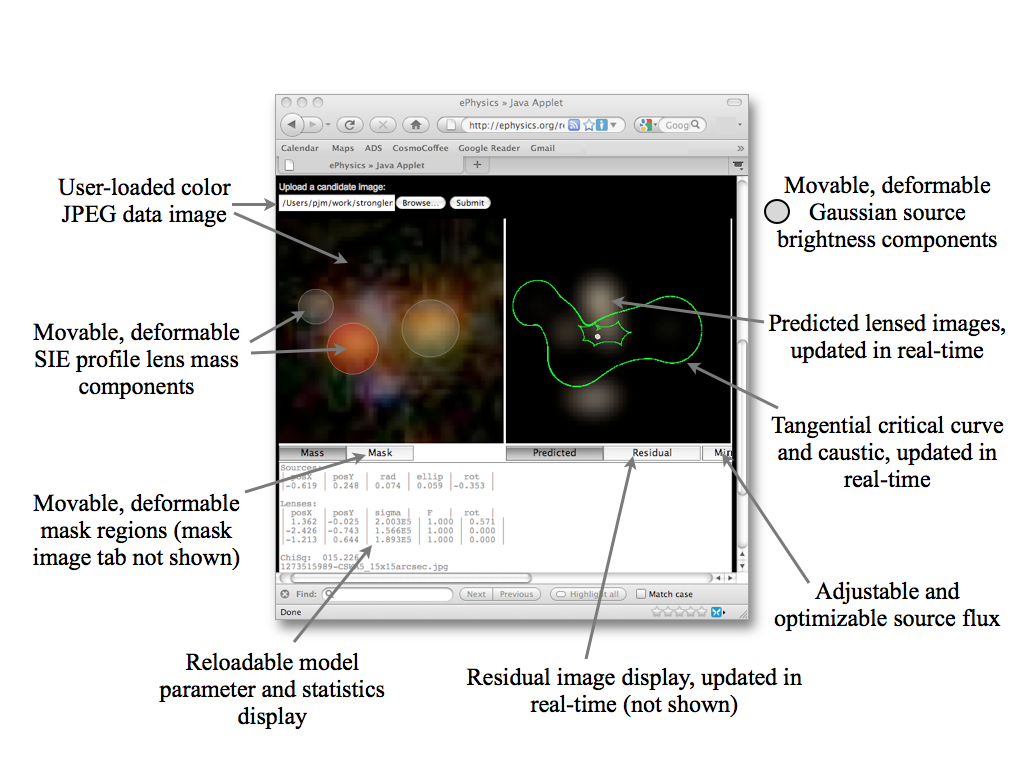
\includegraphics[width=0.9\linewidth]{figs/applet-schematic.eps}
\caption{Screenshot of \theapplet in action. Two image panels show the data
image, with either the pixel mask or mass model overlaid on the left, and the
predicted image (or the residual image) on the right, with the lens caustics
and critical curves, and a representation of the source, overlaid. Underneath the image
panels are displayed the model parameters, and the associated chi-squared.
Other features to note are the image upload box (top) and buttons for
switching between the various viewing options.}
\label{fig:screenshot}
\end{figure*}
%%%%%%%%%%%%%%%%%%%%%%%%%%%%%%%%%%%%%%%%%%

In our approach, the user varies the parameters ``by hand,'' manipulating the
elements of the model directly via a graphical representation of it. 
Figure~\ref{fig:screenshot} shows \theapplet in operation, as a user would see
it on their web browser. As the model is altered, the predicted and residual
images are computed and the display updated in real time, allowing the user to
quickly see the results of their manipulations, and quickly learn what makes a
good model and what does not. Key to this is an appreciation of how the
position of the source relative to the caustic curves influences the system of
multiple images that are produced: this is very difficult to program, but is a
straightforward pattern recognition task for a human operator. For this reason
we continually update the critical curves and caustics in real time. Details
of the modeling procedure we use with our tool are in
Appendix~\ref{sec:manual}.

The brightness of the source is the one parameter we determine automatically,
using one of two methods, selected via a toggled switch.  In the first method,
we rescale the source brightness such that the total  brightness of the unmasked
portions of the astronomical image (in each channel) equals the total brightness
of the same portions of the predicted image. This is very stable, in the sense
that the predicted image always has comparable visibility to the observed image.
In the second method, we rescale the source brightness such that the $\rchisq$
value is minimized: this can be done analytically since the predicted image
brightness depends linearly on the source brightness,  and the observed image is
constant.  Specifically, we rescale each channel's  predicted image by its own
factor $\eta$ where
\begin{align}
\frac{d}{d \eta}\rchisq &\propto 2 \eta \sum_i F_{\text{obs},i} F_{\text{pred},i} - 2 \eta^2 \sum_i F_{\text{pred},i}^2 \\
                        &= 0, \notag \\
\longrightarrow    \eta &= \frac{\sum_i F_{\text{obs},i} F_{\text{pred},i}}
                                {\sum_i F_{\text{pred},i}^2}.
\end{align}
$\eta$ can be computed very quickly, allowing us to  adjust the predicted image
brightness dynamically as the model is varied. However, when the model predicts
the image very badly, the $\rchisq$-optimized brightness is forced to be  very
low. We found that starting with method 1 and then changing to method 2 when the
fit improved gave the best results.

\NEW{Once a good model has been found via manual parameter space exploration, 
the goodness of fit can be automatically optimized. We use the multivariate
Nelder-Mead optimizer provided in the Apache Commons
library.\footnote{http://commons.apache.org}. We found this step  to provide
small but valuable refinements to the model when it is indeed already quite
good; when run while in a region of low goodness of fit, the result can be a
large move to another bad model. This provides some support for the idea that
manual exploration is worthwhile: it is difficult to fit lens models to image
data  automatically, from scratch.}


% ----------------------------------------------------------------------------

\section{The CASSOWARY sample}
\label{sec:sample}

The CASSOWARY sample~\citep{Bel++09} is a list of good candidate  wide
separation gravitational lens systems. The twenty objects used in the present
study comprised the 2008 web-only  release of this catalog. (The sample
continues to grow: by summer 2011, nineteen more objects had been added to
the catalog).  The CASSOWARY objects were found by systematically searching
through the SDSS database for massive ellipticals which appear to be luminous
red galaxies (LRGs) with at least two blue companions lying within $6"$ from the
center of the LRG \citep{Bel++09}.  Candidates were eliminated by constraining
the blue companions to fit certain profiles for size and brightness. Each arc
was required by the team  to have at least two components of comparable
magnitude and a bluer color than is typically found in non-lensing
systems~\citep[][]{Bel++09}. The sample is defined, and  the candidates'
observed properties listed, on the CASSOWARY project
website;\footnote{\texttt{http://www.ast.cam.ac.uk/research/cassowary}} we
reproduce this information in Table~\ref{tab:basic} for the reader's
convenience.

%%%%%%%%%%%%%%%%%%%%%%%%%%%%%%%%%%%%%%%%%%%
\begin{center}
\begin{table*}
\begin{center}
\caption{The CASSOWARY Lens Candidate Sample}
\footnotesize
\renewcommand{\arraystretch}{1.2}
\begin{tabular*}{0.8\linewidth}{@{\extracolsep{\fill}}c c c c cc c}
%%%%%%%
\hline\hline
     ID  &  Name                &  Nickname              &  $\zd$        &  RA\ (degrees)  &  Dec.\ (degrees) &  SDSS phot. ID      \\ \hline
  CSWA1  &  SDSS\ J1148$+$1930  &  The Cosmic Horseshoe  &  0.44$^{a}$   &  177.13811      &  19.50089        &  587742572151374147 \\
  CSWA2  &  SDSS\ J1038$+$4849  &  The Cheshire Cat      &  0.43$^{b}$   &  159.67977      &  48.82195        &  588013382200131773 \\
  CSWA3  &  SDSS\ J1240$+$4509  &  -                     &  0.27$^{b}$   &  190.13452      &  45.15079        &  588017605222793376 \\
  CSWA4  &  SDSS\ J0901$+$1814  &  -                     &  0.35         &  135.34322      &  18.24232        &  588023046402670876 \\
  CSWA5  &  SDSS\ J1244$+$0106  &  -                     &  0.39$^{c}$   &  191.21329      &  1.112080        &  588848901528223970 \\
  CSWA6  &  SDSS\ J1206$+$5142  &  The Clone             &  0.42         &  181.50873      &  51.70820        &  588013382206357664 \\
  CSWA7  &  SDSS\ J1137$+$4936  &  -                     &  0.45         &  174.41690      &  49.60988        &  588295841784725744 \\
  CSWA8  &  SDSS\ J1209$+$2640  &  -                     &  0.56         &  182.34869      &  26.67960        &  587741600957333763 \\
  CSWA9  &  SDSS\ J1227$+$1725  &  -                     &  0.37$^{*}$   &  186.82809      &  17.43108        &  587742902862086260 \\
 CSWA10  &  SDSS\ J2238$+$1319  &  -                     &  0.41         &  339.63048      &  13.33218        &  587730773880078847 \\
 CSWA11  &  SDSS\ J0800$+$0812  &  -                     &  0.31$^{*}$   &  120.05442      &  8.202330        &  587744873710682762 \\
 CSWA12  &  SDSS\ J1133$+$5008  &  -                     &  0.39$^{d}$   &  173.30488      &  50.14447        &  587732484357095512 \\
 CSWA13  &  SDSS\ J1237$+$5533  &  -                     &  0.41         &  189.40086      &  55.56191        &  587731870173298881 \\
 CSWA14  &  SDSS\ J1723$+$3411  &  -                     &  0.44$^{e}$   &  260.90071      &  34.19945        &  587736980648362708 \\
 CSWA15  &  SDSS\ J1008$+$1937  &  -                     &  0.39         &  152.24803      &  19.62124        &  587742014344265970 \\
 CSWA16  &  SDSS\ J1111$+$5308  &  -                     &  0.40$^{*}$   &  167.76458      &  53.14816        &  587731868557115670 \\
 CSWA17  &  SDSS\ J1138$+$2754  &  -                     &  0.33$^{*}$   &  174.53732      &  27.90853        &  587741709956546742 \\
 CSWA18  &  SDSS\ J1134$+$2533  &  -                     &  0.07         &  173.52810      &  25.55977        &  587742191511273514 \\
 CSWA19  &  SDSS\ J0900$+$2234  &  -                     &  0.52$^{*}$   &  135.01103      &  22.56803        &  587741421640024462 \\
 CSWA20  &  SDSS\ J1441$+$1441  &  -                     &  0.74$^{f}$   &  220.45482      &  14.68905        &  587742611340001632 \\
\hline\hline
\end{tabular*}

\raggedright{{\it Notes.} Redshifts come from the SDSS public spectroscopic 
data release DR7 \citep{DR7} unless marked as follows:  
$^a$\citet{Bel++07},
$^b$\citet{Dye++08},
$^c$\citet{Chr++10},
$^d$\citet{San++05},
$^e$\citet{Kub++10},
$^f$\citet{Pet++10}.
An asterisk $^{*}$ indicates a DR7 photometric redshift.
The two brightest lens galaxies in CSWA~5, CSWA~15 and CSWA~16 have
different redshifts (although for CSWA~16 these are photo-z's) -- 
given here are the arithmetic means of the
two values.}
\normalsize
\vspace{\baselineskip}

\label{tab:basic}
\end{center}
\end{table*}
\end{center}
%%%%%%%%%%%%%%%%%%%%%%%%%%%%%%%%%%%%%%%%%%

Half of the 20 
CASSOWARY systems considered here have been confirmed by some combination of
detailed modeling, high resolution imaging, and
spectroscopy~\citep{Bel++07,Bel++09,Pet++10}.  Indeed, several were discovered
and followed up independently as part of the SDSS Bright Arcs Survey
\citep[\eg][]{Lin++09,Die++09,Kub++09,Kub++10}.  To date, spectroscopic
redshifts have been obtained for the lenses and arcs in CSWA~1--8, CSWA~14 and
CSWA~20,  showing the blue images to be of background high redshift galaxies,
distorted by the lens. The strong lensing -- \ie multiple-imaging -- nature of
the deflectors has been confirmed in some, but not all  of these cases, via
modeling of  follow-up imaging data. Plausible models have therefore  not been
made for all systems; without such a model, it remains inconclusive whether they
really are strong gravitational lenses, \ie causing multiple imaging of a
background object. 

We analyzed both JPEG and FITS images of the candidates.   In most cases, we
used the SDSS SkyServer JPEG, as used in the Galaxy Zoo project \citep{gz1}.
However, in some cases the low surface brightness arcs did not appear with
sufficient contrast: in these cases we made use of the JPEG image provided by
the CASSOWARY team on their website,  which are in general clearer and
brighter than those provided by SDSS, having been individually optimized for
visibility. By default, a simple circularly-symmetric Gaussian of FWHM 1.4''
was assumed to approximate the SDSS PSF. The field of view of the image must
also be specified to allow the JPEG image pixel scale to be computed.
\NEW{Small ``postage stamp'' images were excised from the FITS images
downloaded from the Skyserver website; these contain the PSFWID keyword and
value in their headers, which we used in our Gaussian PSF model.  Lastly, we
note that all the images in this paper are oriented such that North is up and
East is left.}


% ----------------------------------------------------------------------------

\section{Results}
\label{sec:results}

In this section, we first present the results of our \theapplet modeling of the
CASSOWARY sample, providing details of the manual models for each system in
turn, and compare them with those in the literature where possible. We then 
go on to discuss the properties of the sample as a whole.

%  -  -  -  -  -  -  -  -  -  -  -  -  -  -  -  -  -  -  -  -  -  -  -  -  -  

\subsection{Notes on individual systems}
\label{sec:results:indi}

In Figures~\ref{fig:cswa1}--\ref{fig:cswa20} below, we show two models for each
of the CASSOWARY lens candidates. The first model has been optimized to the
SDSS multi-filter JPEG data image, while the second model has been optimized
to the SDSS FITS image. Each model is accompanied by the predicted lensed image
and, corresponding image residual, for our best \theapplet model.  The caustics
and critical curves for this lens model are overlaid. By analyzing the $\Omega$
values of JPEG and FITS models, no trend was noticed which could indicate that
FITS models are better than JPEG models.

% . . . . . . . . . . . . . . . . . . . . . . . . . . . . . . . . . . . .  .  

\subsubsection*{CSWA~1: SDSS\ J1148$+$1930}
\label{sec:results:indinotes:cswa1}

% {\bf CLASSIFICATION: A}

%%%%%%%%%%%%%%%%%%%%%%%%%%%%%%%%%%%%%%%%%%
\begin{figure}[!ht]
	\centering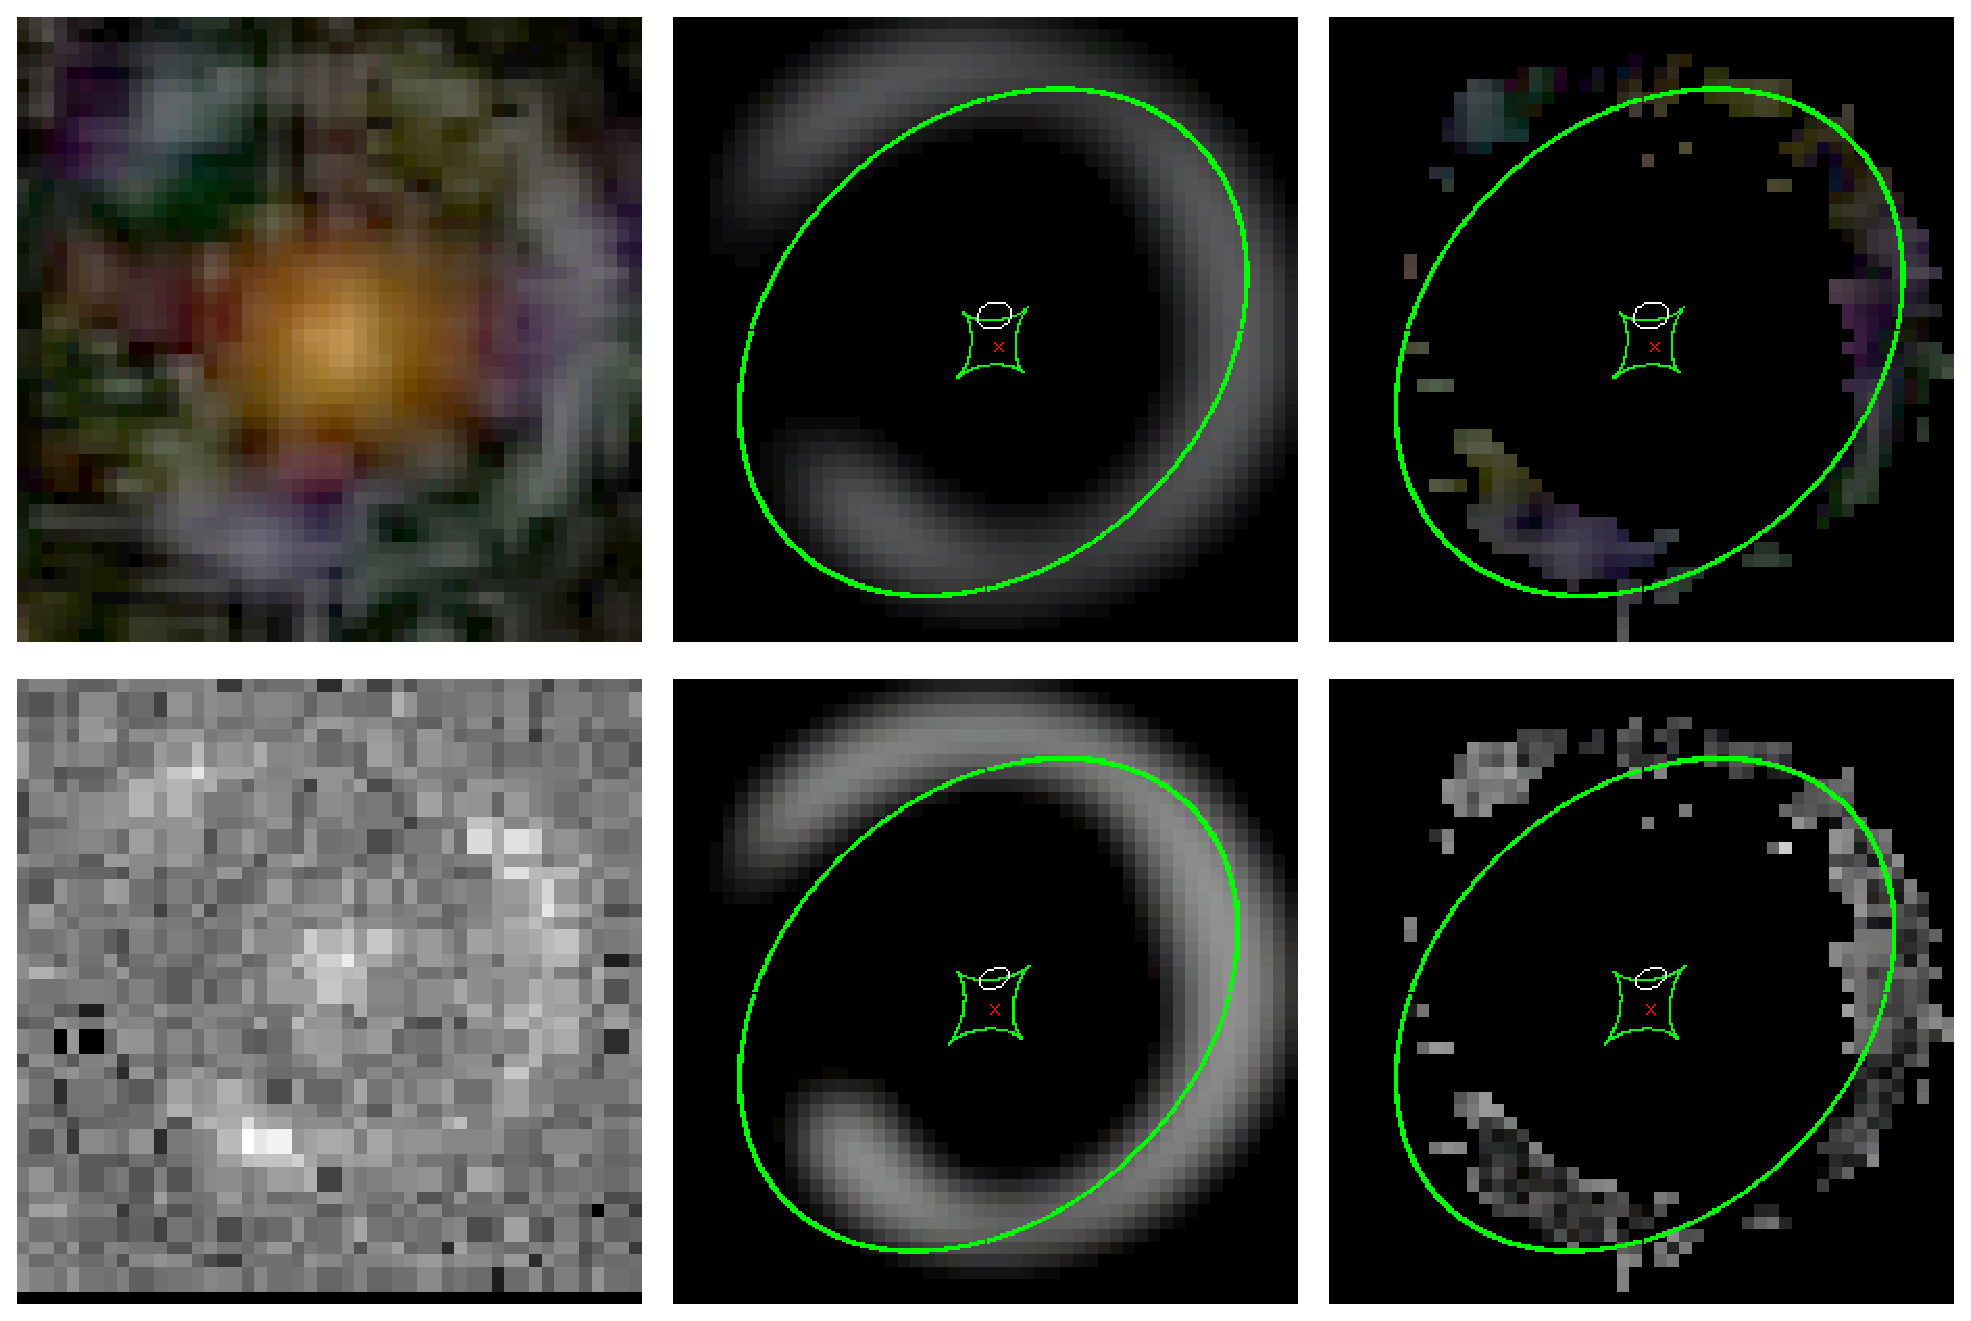
\includegraphics[width=\linewidth]{figs/1.eps}
	\caption{CSWA 1. Top panels: models optimized to SDSS color JPEG image;
	Bottom panels: models optimized to SDSS FITS image.  Left: SDSS data image;
	Center: model-predicted image; Right: residual image. In this and subsequent
	figures, the lens model tangential 
	critical curve and caustics are shown overlaid in green, the lens component
	centroids as red crosses, and the source positions as white circles. 
	The residual image
	is zero where the data were masked.}
	\label{fig:cswa1}
\end{figure}
%%%%%%%%%%%%%%%%%%%%%%%%%%%%%%%%%%%%%%%%%%

This lens candidate, also known as ``The Cosmic Horseshoe,''  is a simple
lensing system with a very bright, nearly complete, Einstein ring
\citep{Bel++07}. These authors showed that CSWA~1 consists of a high-redshift
star-forming galaxy being strongly lensed by a massive early-type galaxy (likely
the brightest, dominant central member of a group),  which, when modeled with a
SIE mass distribution was found to have a velocity dispersion parameter of 
$\sigmaSIE \sim 500 \kms$ \citep{Dye++08}. 

Our \theapplet lens model, made independently,  agrees well with the SIE model
presented \citep{Dye++08}, both in terms of Einstein radius and lens ellipticity
and orientation.  Using the redshifts of the source and lens galaxies presented
in \citet{Bel++07}, we translated our Einstein radius into a velocity dispersion
of $\sigmaSIE = 506 \pm 5 \kms$.

The SIE lens model velocity dispersion  is in agreement with the spectroscopic
velocity dispersion measured by \citet{Bel++07} of  $\sigma_{\rm v} = 430 \pm 50
\kms$, but significantly higher than the more recent and more accurate 
measurement by \citet{Spi++11} of $\sigma_{\rm v} = 351 \pm 10 \kms$. From a
more detailed lens model, \citet{Dye++08} found that the density profile {\it
at} the Einstein radius  is very close to isothermal; \citet{Spi++11} concluded
from  their lower stellar velocity dispersion that the density profile {\it
within} the Einstein radius must be shallower than isothermal. This illustrates
the way that SIE models provide satisfactory fits to  lensed image data, even if
the actual lens density profile is more complex than this.

The factor of $23 \pm 10$ magnification that our model predicts is lower than
the $\sim 50$ magnification found by \citep{Bel++07}. This is partially a result
of our inferred source size being larger: 0.55 arcsec compared to the $\simeq
0.3$~arcsec found by \citet{Dye++08}. We found that changing the source size
could be offset by increasing the PSF to $1.8''$, although this model has a
marginally lower goodness of fit ($\Omega$ decreases from 80\% to  76\%).

% . . . . . . . . . . . . . . . . . . . . . . . . . . . . . . . . . . . .  .  

\subsubsection*{CSWA~2: SDSS\ J1038$+$4849}
\label{sec:results:indinotes:cswa2}

% {\bf CLASSIFICATION: A}

%%%%%%%%%%%%%%%%%%%%%%%%%%%%%%%%%%%%%%%%%%
\begin{figure}[!ht]
	\centering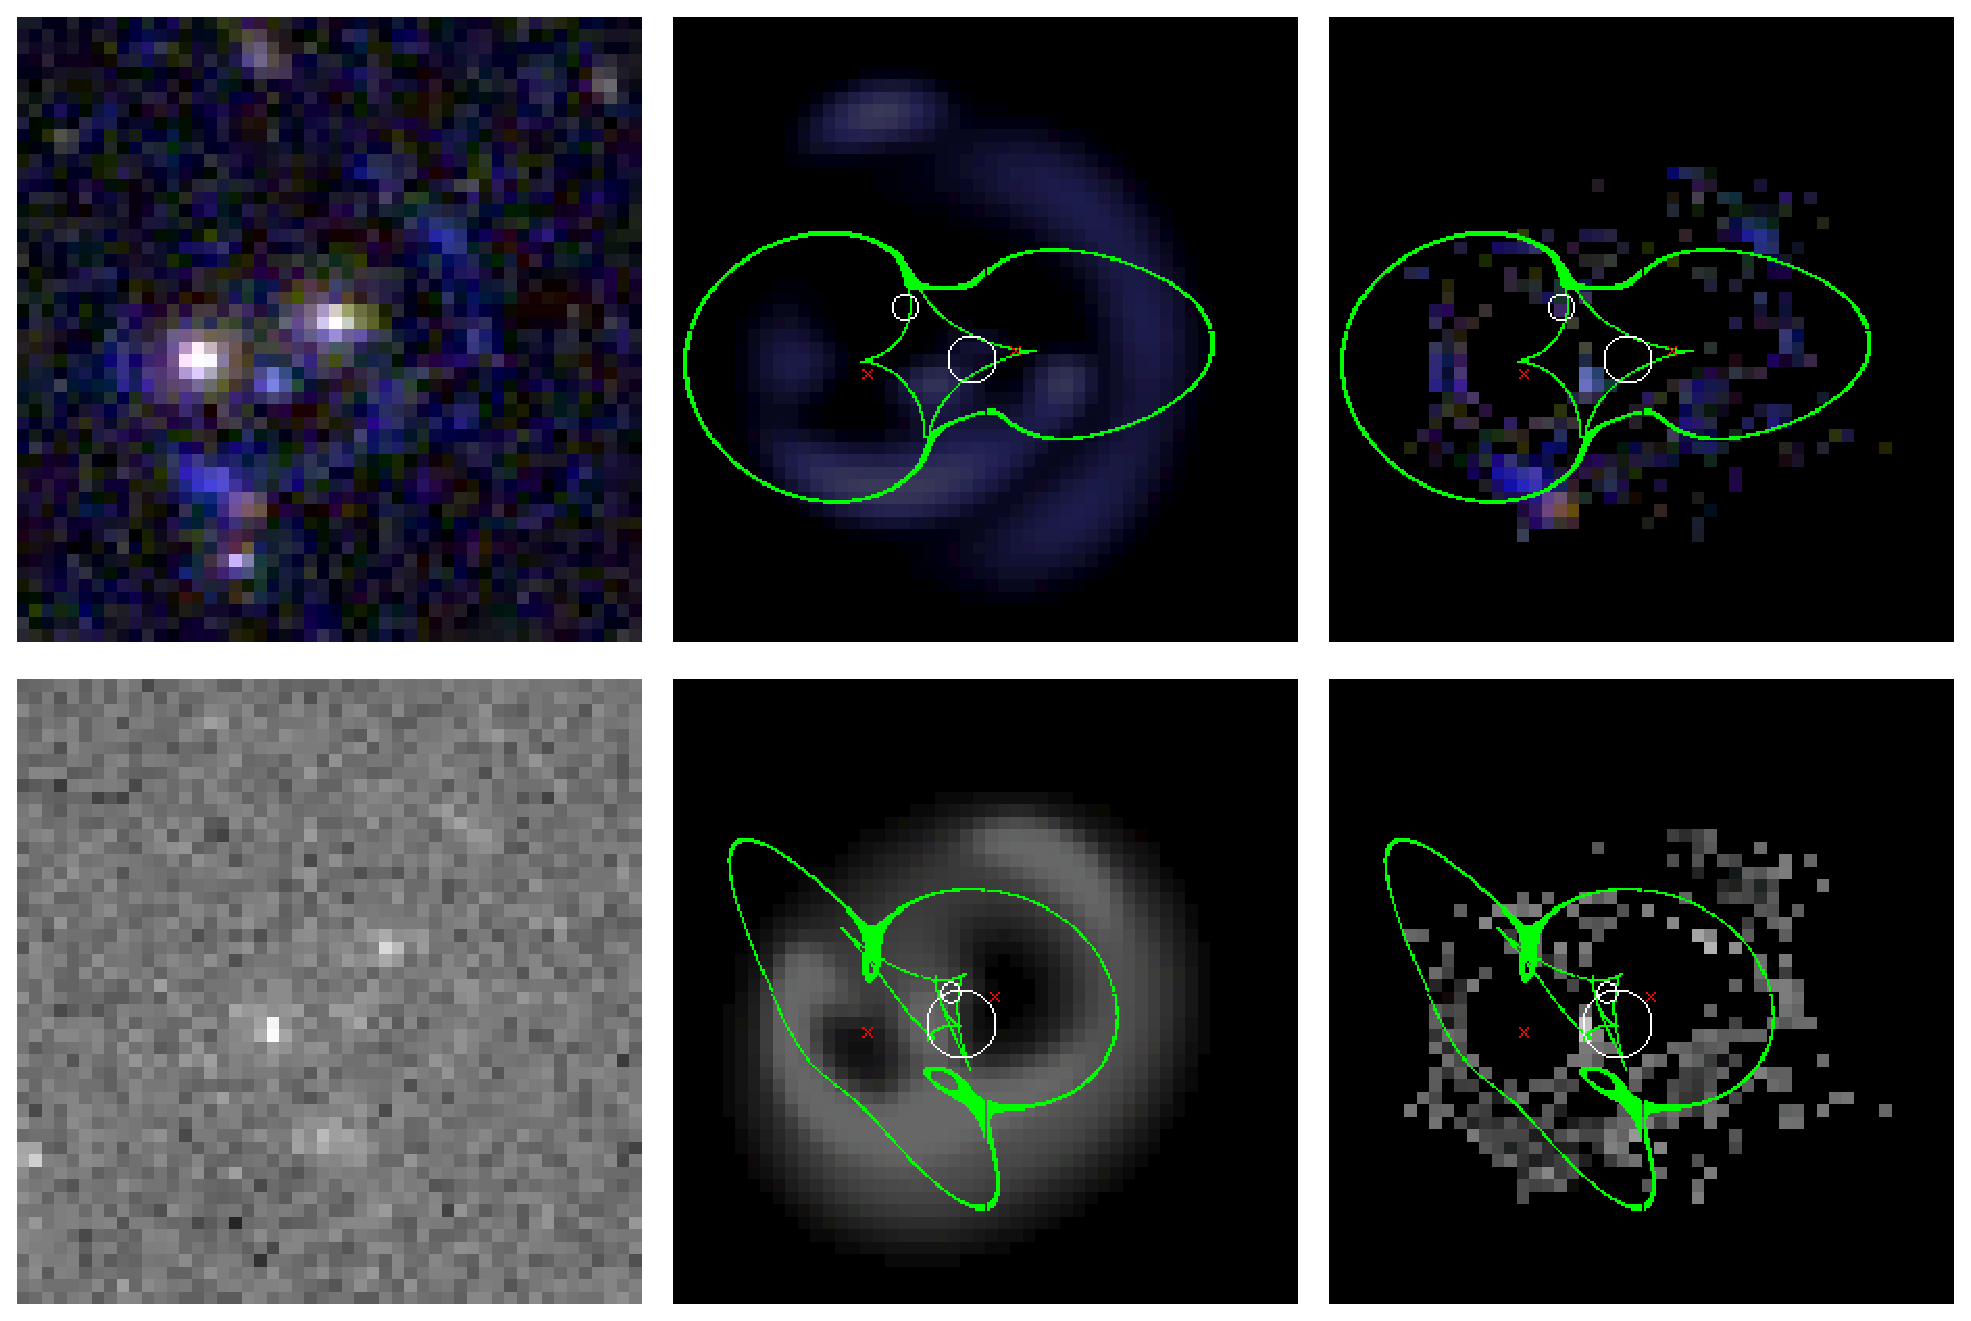
\includegraphics[width=\linewidth]{figs/2.eps}
	\caption{CSWA 2, see Figure~\ref{fig:cswa1} for caption.}
	\label{fig:cswa2}
\end{figure}
%%%%%%%%%%%%%%%%%%%%%%%%%%%%%%%%%%%%%%%%%%

This confirmed lens, referred to by the CASSOWARY team as ``The Cheshire Cat,''
is a projection of two galaxies (the ``eyes'' of the Cat) that is lensing  two
sources, resulting in two bright arcs \citep{Bel++09}.  The two lens galaxies
have similar redshifts ($z=0.426$ and $0.432$), suggesting that our single lens
plane assumption might be sufficient.  The two sources, however, have quite
different redshifts \citep[$z=0.97$ and $z>1.4$][]{Bel++09}.  We do find a
two-component model that predicts images that partially fit the two arc systems,
although the residuals are significant ($\Omega = 26\%)$.  In particular, we
predict counter-images in slightly the wrong places. We ascribe some of these
difficulties to the multiple lens and source plane redshifts. Nevertheless, our
ability to reproduce the brightest and most distorted  parts of the arcs
supports the strong lensing hypothesis for this system.

\citeauthor{Bel++09} do not present a lens model, but do give an estimated
magnification of the $ 45 \pm 7$. This is somewhat higher than our estimate of
$17 \pm 7$, possibly as a consequence of the small discrepancies between models,
as discussed above.

% . . . . . . . . . . . . . . . . . . . . . . . . . . . . . . . . . . . .  .  

\subsubsection*{CSWA~3: SDSS\ J1240$+$4509}
\label{sec:results:indinotes:cswa3}

% {\bf CLASSIFICATION: A}

%%%%%%%%%%%%%%%%%%%%%%%%%%%%%%%%%%%%%%%%%%
\begin{figure}[!ht]
	\centering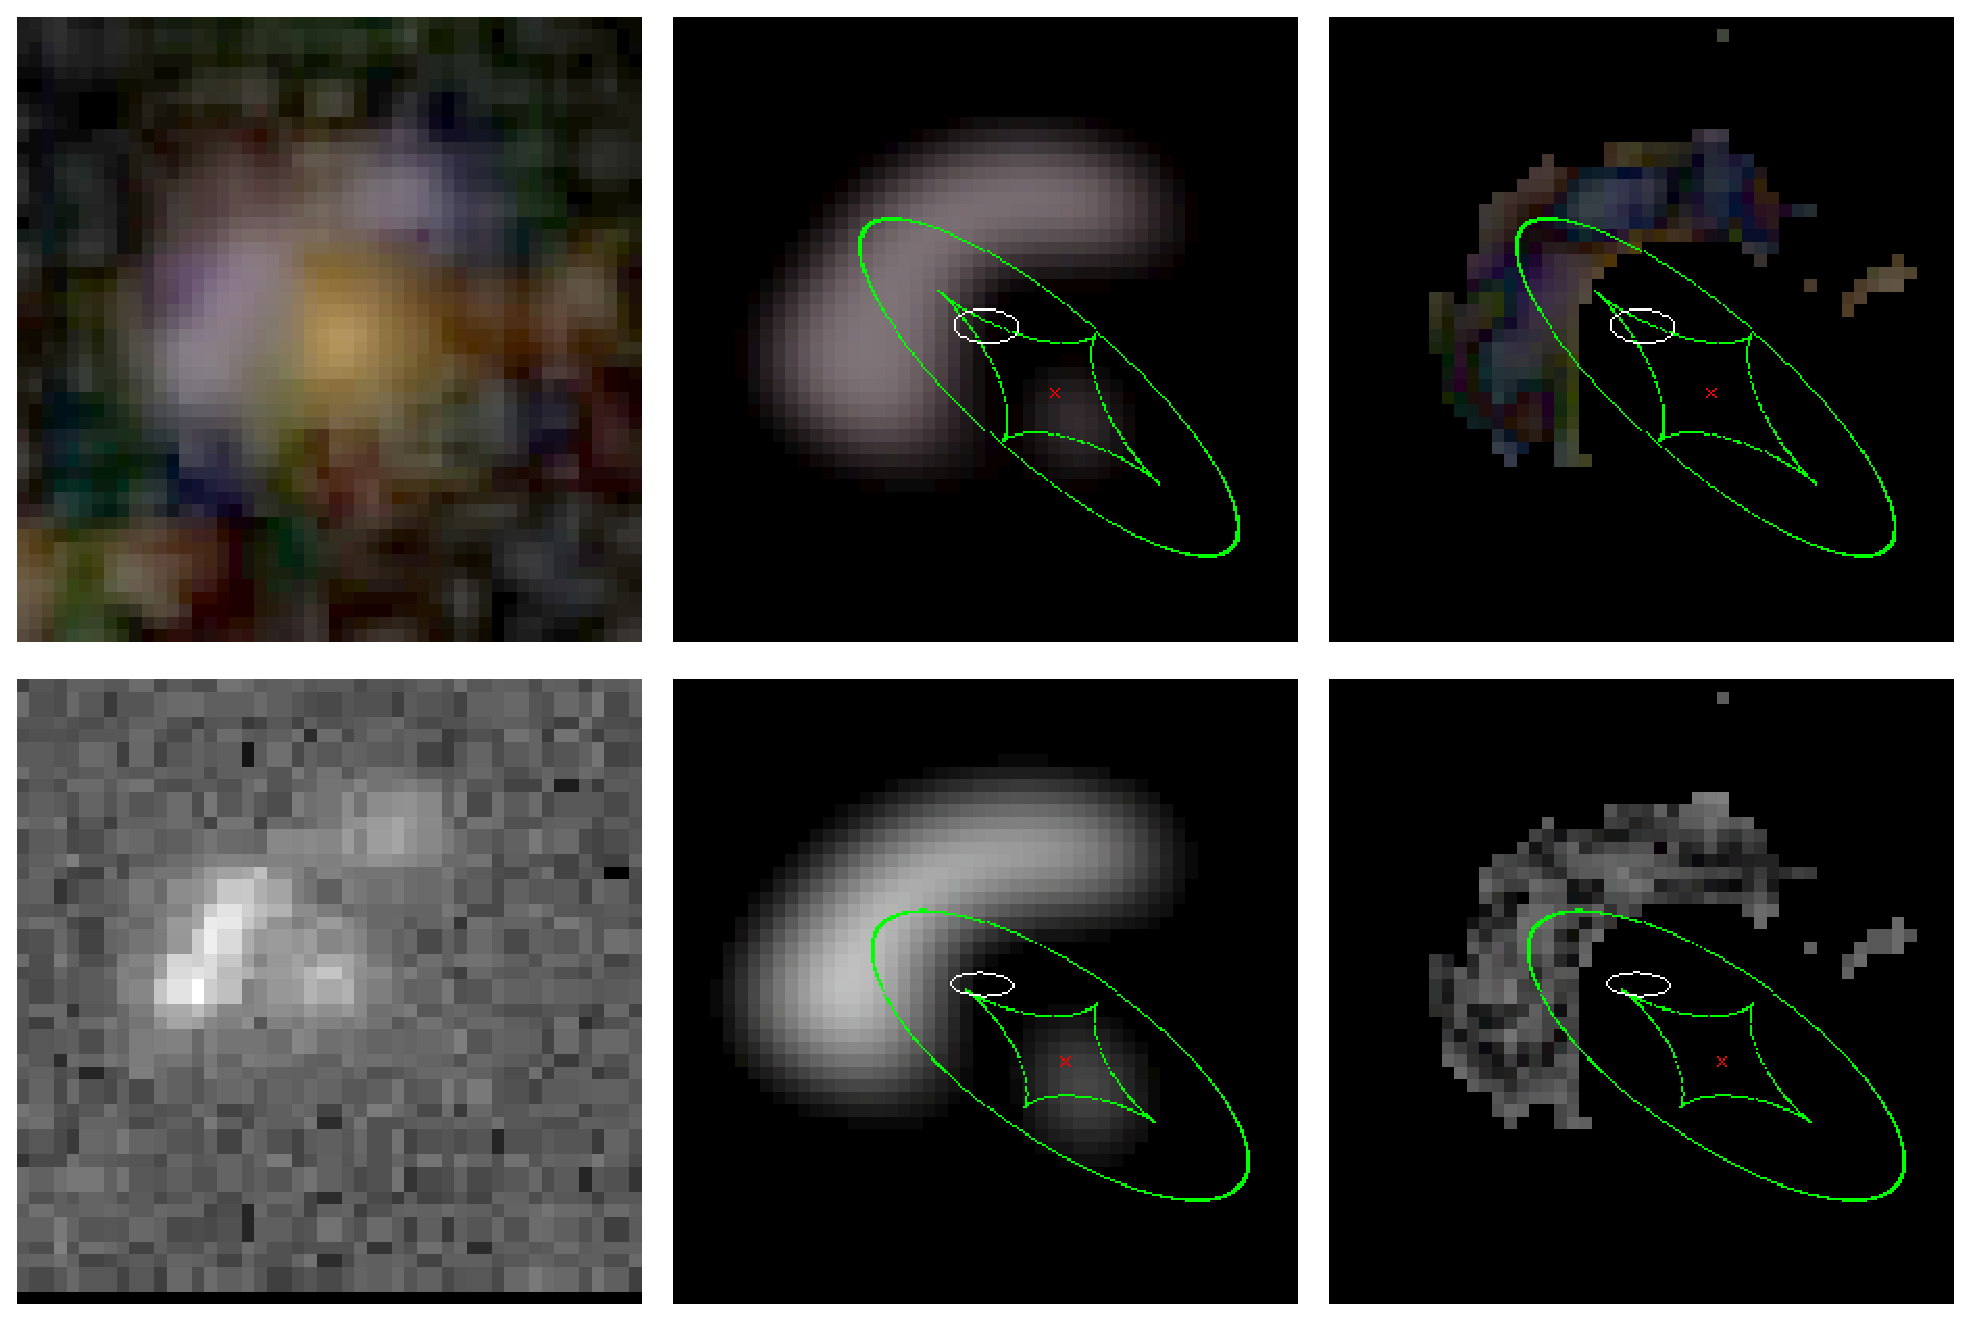
\includegraphics[width=\linewidth]{figs/3.eps}
	\caption{CSWA 3, see Figure~\ref{fig:cswa1} for caption.}
	\label{fig:cswa3}
\end{figure}
%%%%%%%%%%%%%%%%%%%%%%%%%%%%%%%%%%%%%%%%%%

CSWA~3 consists of a typical star-forming galaxy lensed by a early-type galaxy,
and was also discussed by \citet{Bel++09}. The magnification of our model ($7
\pm 2$) is again rather lower than  the $\sim 18 \pm 3$ they  found. 

The distinctive brightness and curvature of the main arc is very  strong
evidence for this system being a lens -- indeed, our best model predicts the arc
to be three merging images.  Although our faint residual image indicates good
agreement between the predicted and astronomical images, we note that our model
does predict  a rather  high lens ellipticity: the light distribution of the
lens is much less elongated.  Attempts at modeling this candidate with a lens
mass distribution  of lower ellipticity were unsuccessful, even when multiple
sources were used; these alternative models all feature more prominent
counter-arcs which are clearly not present in the data image.   


% . . . . . . . . . . . . . . . . . . . . . . . . . . . . . . . . . . . .  .  

\subsubsection*{CSWA~4: SDSS\ J0901$+$1814}
\label{sec:results:indinotes:cswa4}

% {\bf CLASSIFICATION: B}

%%%%%%%%%%%%%%%%%%%%%%%%%%%%%%%%%%%%%%%%%%
\begin{figure}[!ht]
	\centering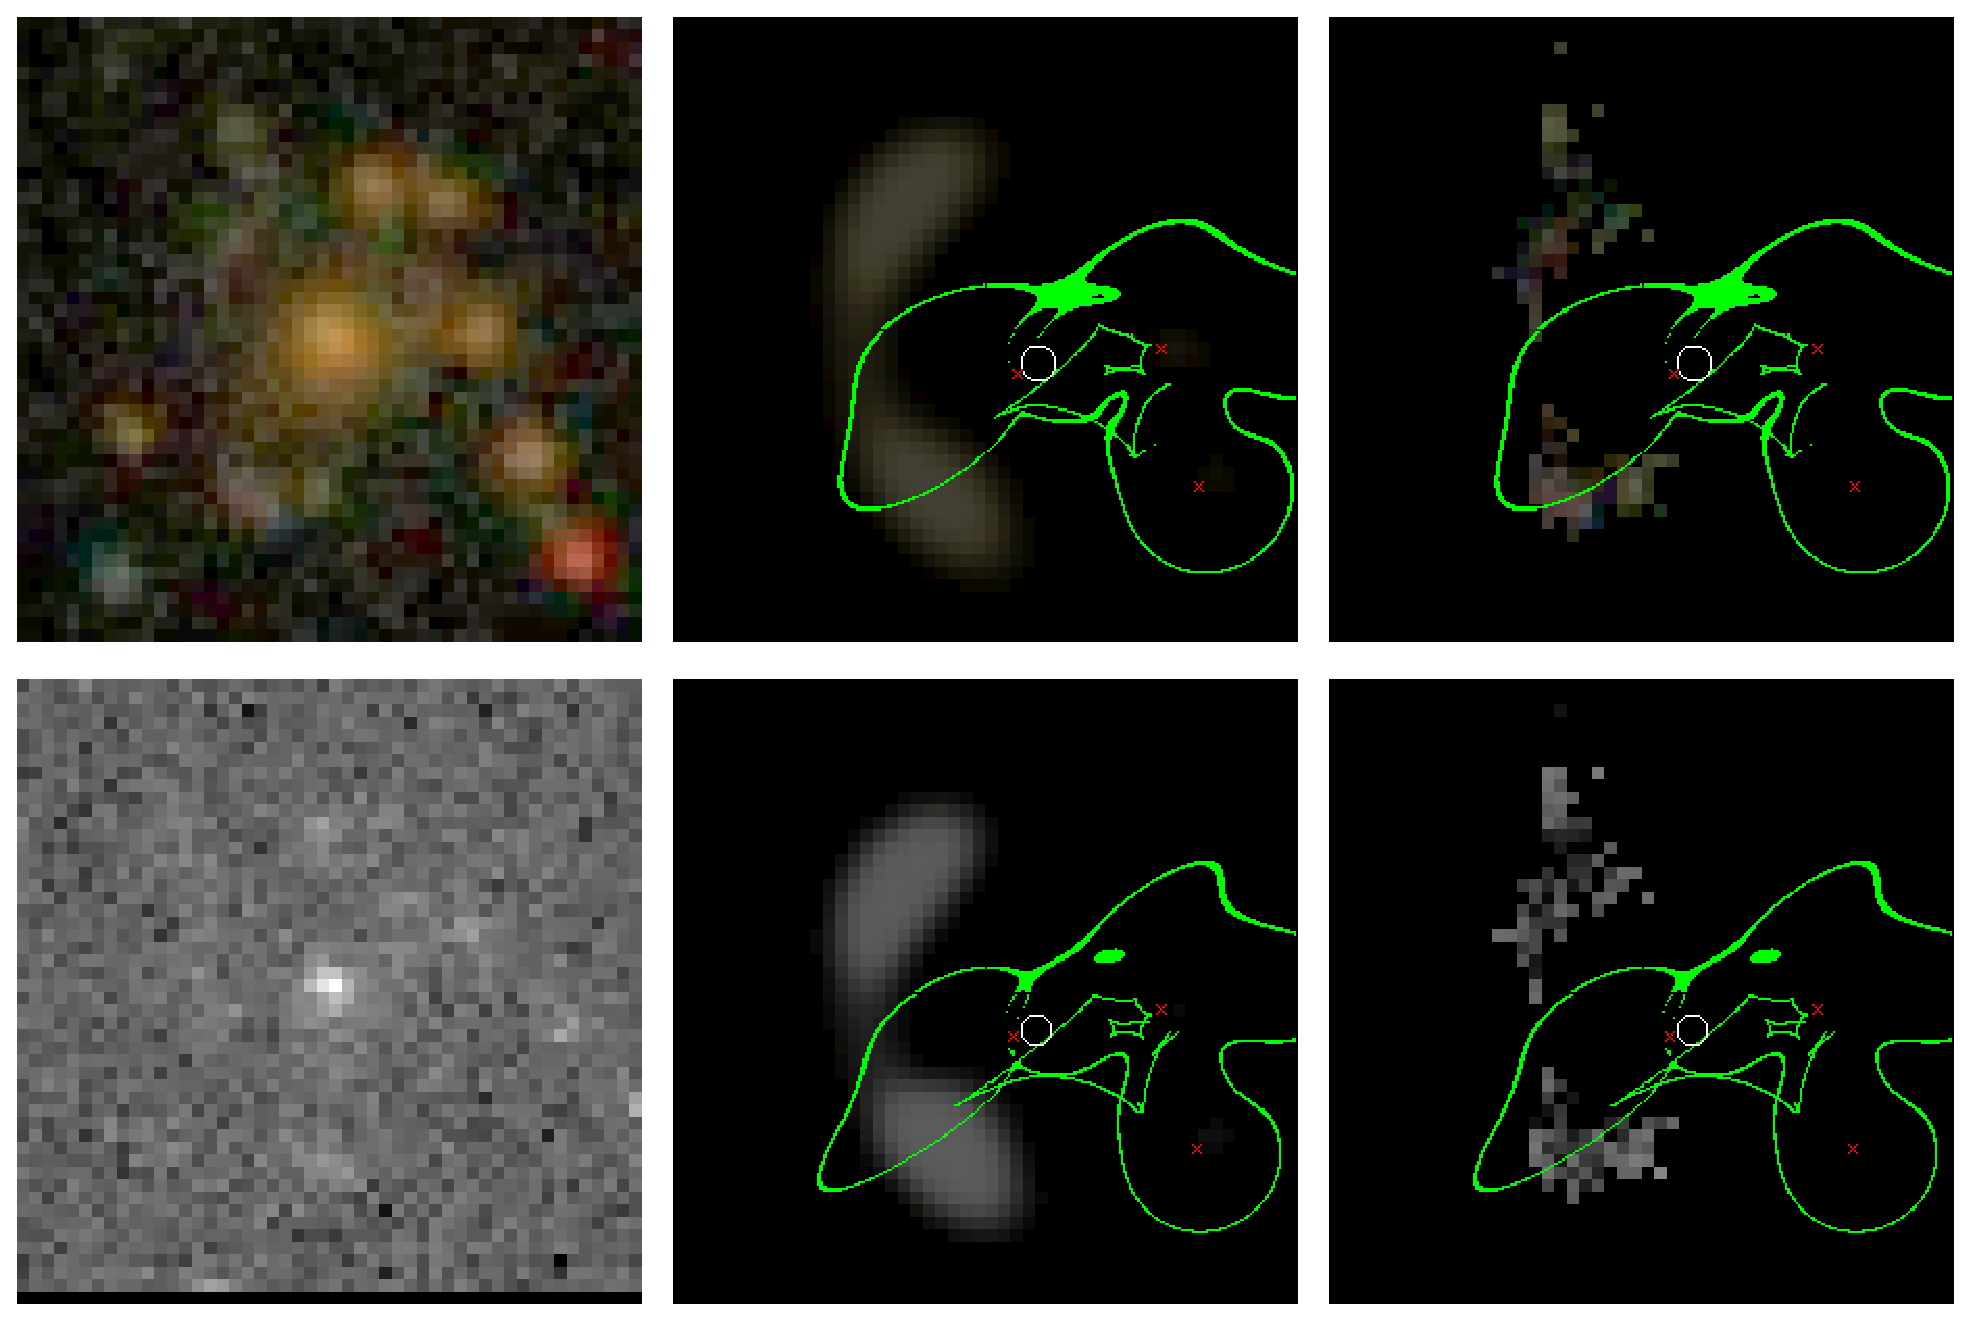
\includegraphics[width=\linewidth]{figs/4.eps}
	\caption{CSWA 4, see Figure~\ref{fig:cswa1} for caption.}
	\label{fig:cswa4}
\end{figure}
%%%%%%%%%%%%%%%%%%%%%%%%%%%%%%%%%%%%%%%%%%

\citet{Bel++07} have shown that CSWA~4 consists of a central LRG with many
nearby galaxies in the same cluster. Three of these galaxies lie within $10"$ of
the central galaxy. This complicated lens candidate was briefly discussed by
\citet{Die++09}.  Independently, we were able to assign mass to each of the 4
central lens galaxies and predict the North-east and South-east arcs, along with
a counter-image to the West (slightly offset from its observed position),  with
a single quadruply-imaged source.  The morphology of these arcs is not as well
predicted as their position, again suggesting that a more exhaustive search of
parameter space is required to obtain a more  accurate model of the detailed
lens mass structure. In particular, our model predicts the South East arc to be
long, composed of 2 merging images, while  the observed arc is rather shorter. 


% . . . . . . . . . . . . . . . . . . . . . . . . . . . . . . . . . . . .  .  

\subsubsection*{CSWA~5: SDSS\ J1244$+$0106}
\label{sec:results:indinotes:cswa5}

% {\bf CLASSIFICATION: A}

%%%%%%%%%%%%%%%%%%%%%%%%%%%%%%%%%%%%%%%%%%
\begin{figure}[!ht]
	\centering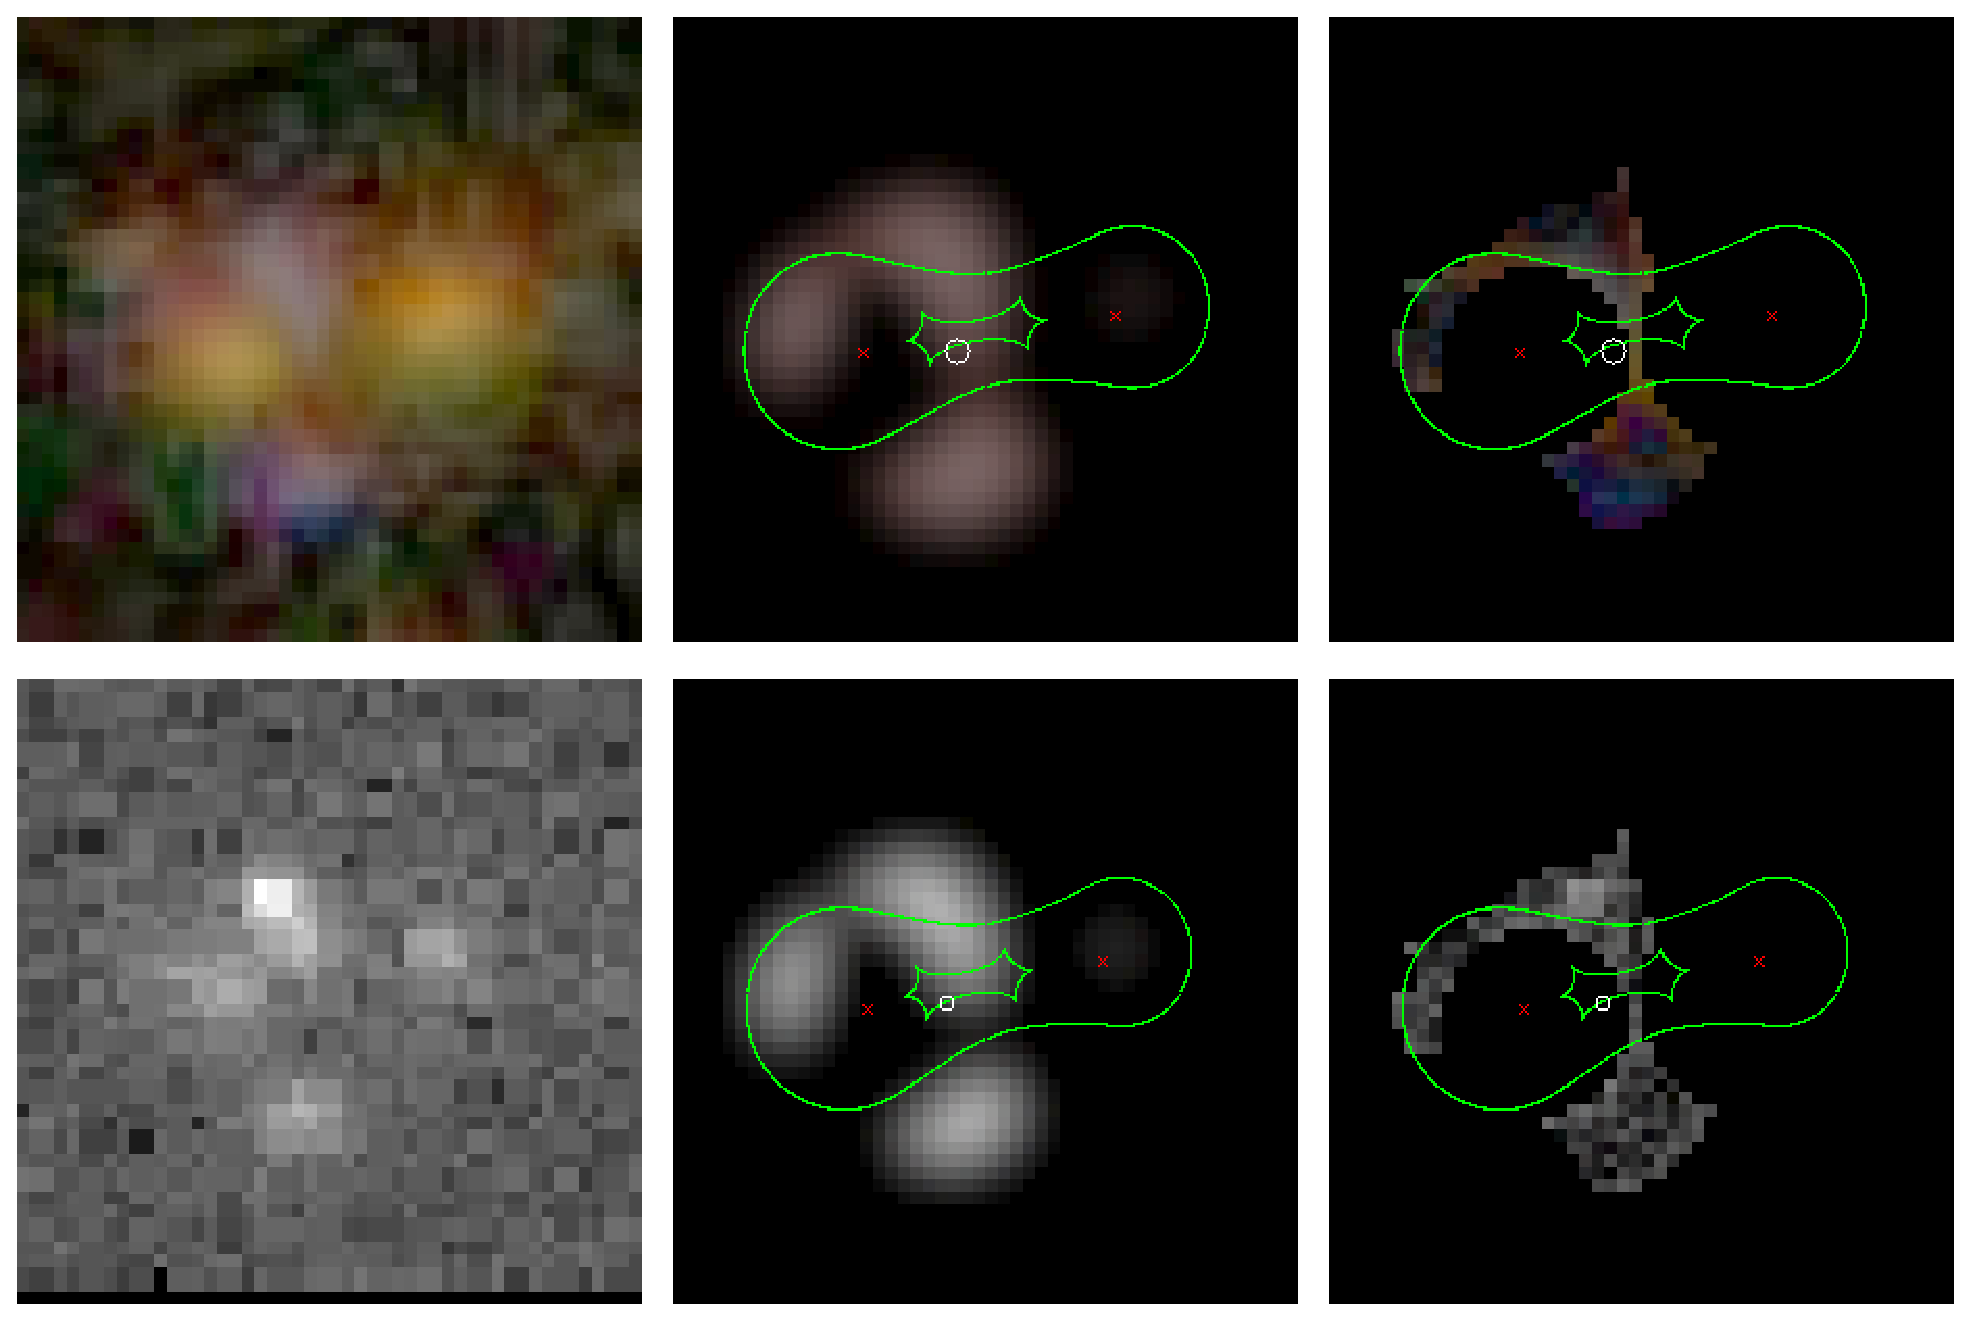
\includegraphics[width=\linewidth]{figs/5.eps}
	\caption{CSWA 5, see Figure~\ref{fig:cswa1} for caption.}
	\label{fig:cswa5}
\end{figure}
%%%%%%%%%%%%%%%%%%%%%%%%%%%%%%%%%%%%%%%%%%

\citet{Bel++07} showed that CSWA~5 consists of a blue star-forming galaxy,
lensed by a group (or possibly a line of sight superposition)  of red galaxies.
As seen in the SDSS survey image, the  system consists of two bright red lens
galaxies, a faint red satellite nearby, and a bright blue arc and a possible
blue counter-image.   With slightly higher resolution data, \citet{Chr++10}
found  a fourth blue image to the East of the system (not seen in the SDSS
image), and suggest that the arc is actually two merging images.  They then
confirmed that the three images which are roughly aligned vertically have been
confirmed to be from the same source, but could not confirm that the fourth,
Eastern image is also of this source~\citep{Chr++10}. We find models that
reproduce all four images using a single source, by assigning mass to both the
bright red galaxies. A better prediction of the position of the  fourth image
can be obtained by including the faint lens satellite to the North-East as a
third mass component.

\citet{Chr++10} measured the velocity dispersion of the Western lens to be 278
km/s and its redshift to be $z = 0.3877$. (The redshifts and velocity
dispersions are expected to be similar for the Eastern lens).  \citet{Chr++10}
also determined the redshift of the source to be $z=1.0686$.  Using these
redshifts, we determined the velocity dispersion of the Western lens, according
to our model, to be $330\pm10$~km/s. Some of this discrepancy is likely due to
the difference between the SIE normalisation parameter and the observed
aperture spectral velocity dispersion, possibly as a result of a
non-isothermal to the mass distribution in the core.

\NEW{While this paper was being refereed, \citet[][CG11]{C+G11} published an
analysis of CSWA5, finding a very similar binary lens model, with the Einstein
radii of the Western and Eastern lenses of 2.01 and 1.75 arcsec respectively.
These values are very similar to those we found, but are transposed.
\citet{C+G11} note that there is significant anticorrelation between these two
parameters' error distributions. This is likely to affect both analyses:
\theapplet fits all the pixels in the image, but with an approximate PSF
model, while CG11 assume point-like images. The latter assumption may explain
the discrepancy between the \theapplet magnification estimates of 9-13,
compared to CG11's 17: the point source approximation will tend to
over-estimate the magnification estimate.}


% . . . . . . . . . . . . . . . . . . . . . . . . . . . . . . . . . . . .  .  

\subsubsection*{CSWA~6: SDSS\ J1206$+$5142}
\label{sec:results:indinotes:cswa6}

% {\bf CLASSIFICATION: A}

%%%%%%%%%%%%%%%%%%%%%%%%%%%%%%%%%%%%%%%%%%
\begin{figure}[!ht]
	\centering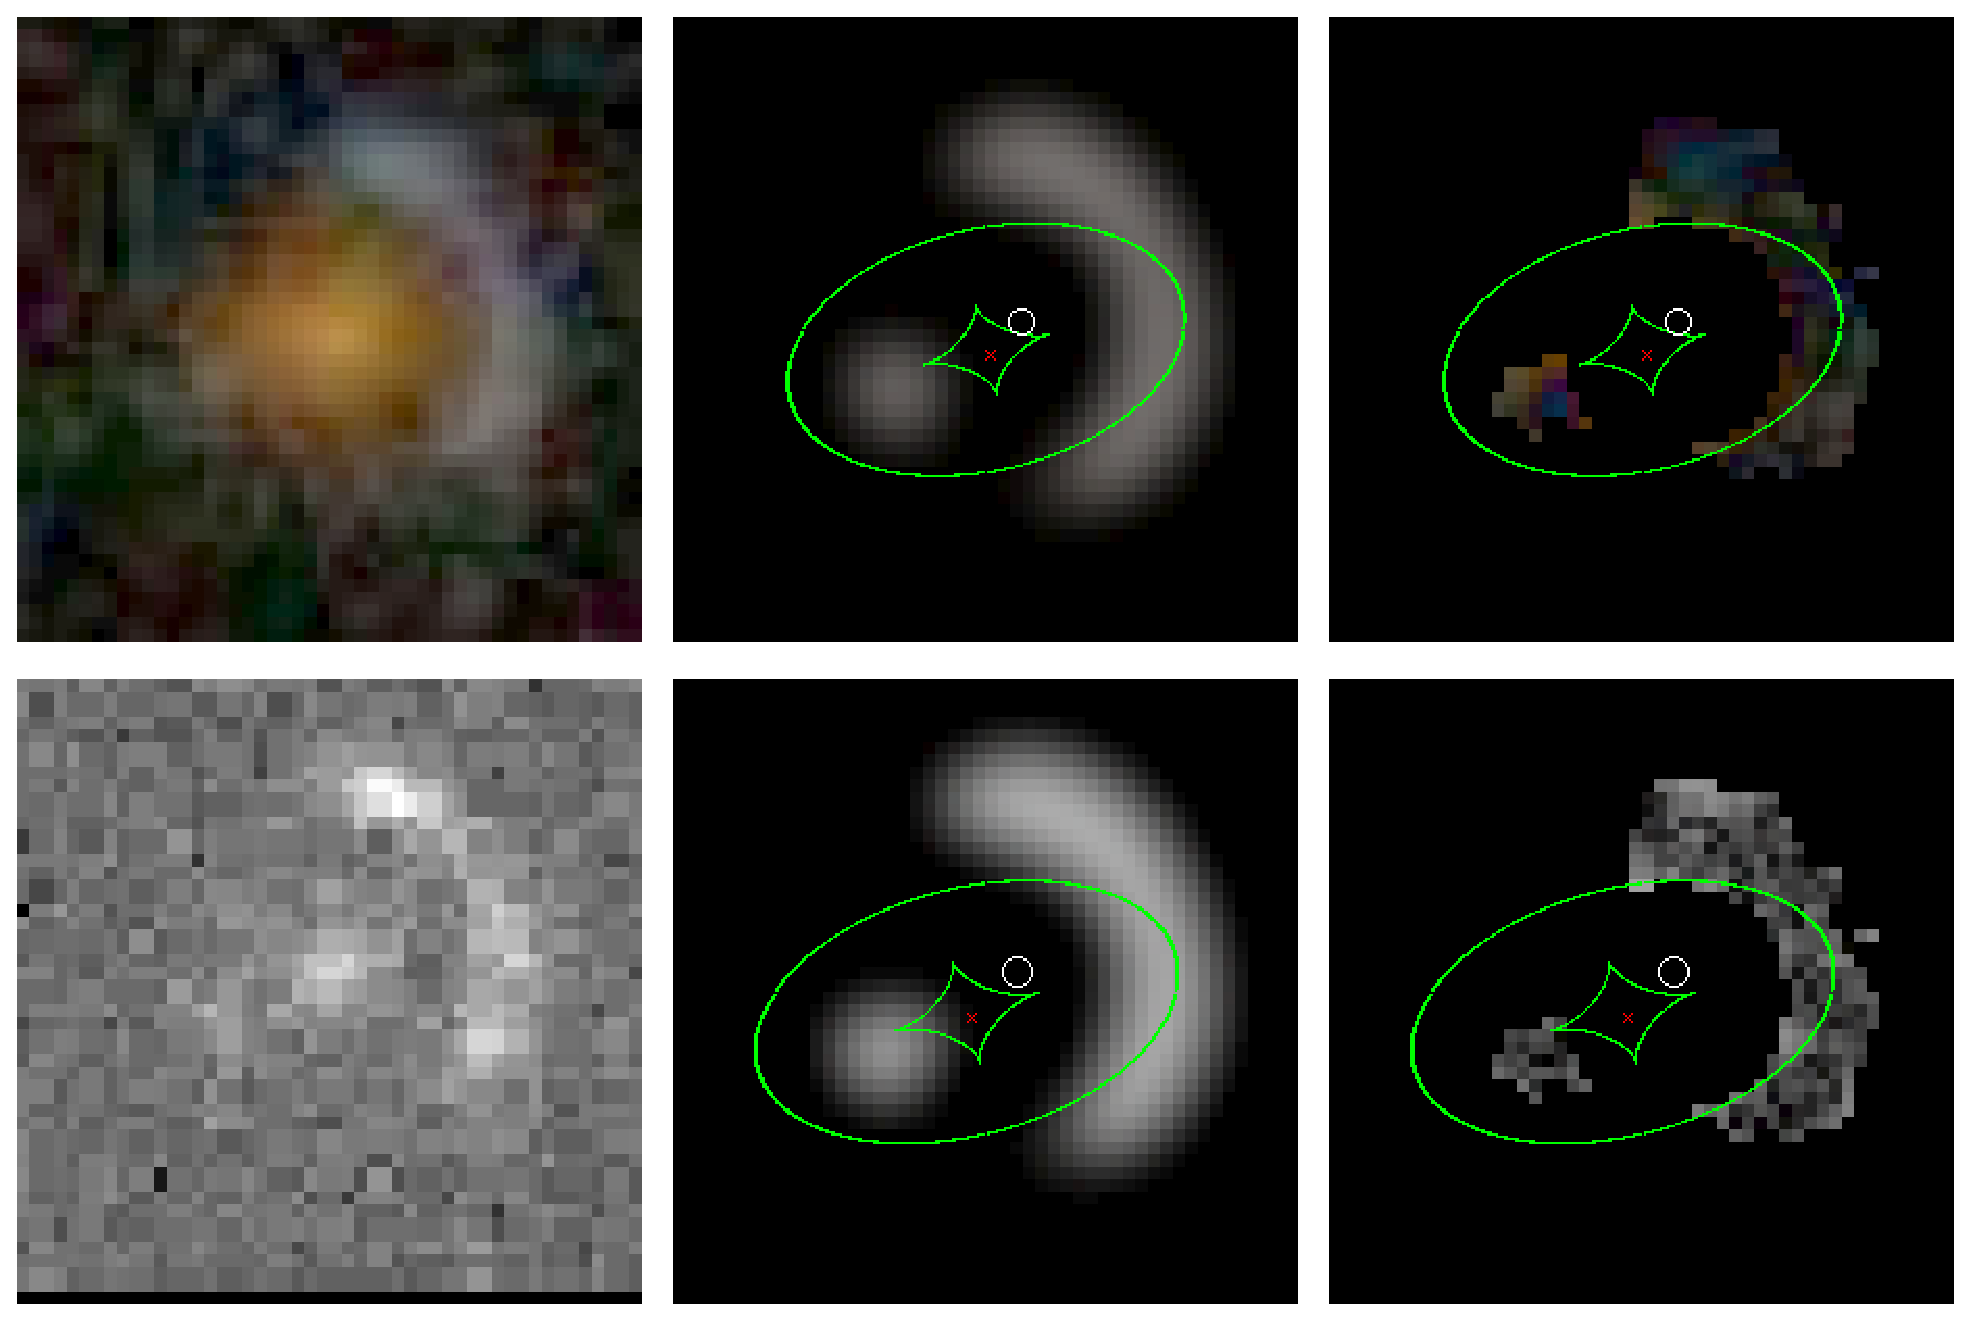
\includegraphics[width=\linewidth]{figs/6.eps}
	\caption{CSWA 6, see Figure~\ref{fig:cswa1} for caption.}
	\label{fig:cswa6}
\end{figure}
%%%%%%%%%%%%%%%%%%%%%%%%%%%%%%%%%%%%%%%%%%

This lens candidate, referred to in the literature  as The Clone, is a simple
single-lens system. From follow-up imaging,  \citet{Lin++09} determined the
Einstein radius to be $3.82 \pm 0.03$~arcsec and the magnification to be $27 \pm
1$. We are also able to model the arc and its counter-image, finding an Einstein
radius in good agreement ($3.8\pm0.1$~arcsec). We again note that the \theapplet
lens magnification is low compared to the value in the literature, at $14\pm6$,
possibly due to the PSF width--source size degeneracy.


% . . . . . . . . . . . . . . . . . . . . . . . . . . . . . . . . . . . .  .  

\subsubsection*{CSWA~7: SDSS\ J1137$+$4936}
\label{sec:results:indinotes:cswa7}

% {\bf CLASSIFICATION: B}

%%%%%%%%%%%%%%%%%%%%%%%%%%%%%%%%%%%%%%%%%%
\begin{figure}[!ht]
	\centering\includegraphics[width=\linewidth]{figs/7.eps}
	\caption{CSWA 7, showing models with one source (top row) and 2 sources
      (bottom row). Otherwise see Figure~\ref{fig:cswa1} for caption.}
	\label{fig:cswa7}
\end{figure}
%%%%%%%%%%%%%%%%%%%%%%%%%%%%%%%%%%%%%%%%%%

This lens candidate  was selected, followed up and analyzed by \citet{Kub++09},
who determined it to consist of a single lens and  two spatially-unresolved
sources (the latter piece of information coming from their optical
spectroscopy). The brightest blue image component  lies at 3.7~arcsec from the
putative lens galaxy. For this reason, we present two models of this lens
candidate -- one (7a)  with a single source ($\Rein = 2.6\pm0.2$''), and one
(7b) with two sources  ($\Rein = 2.9\pm0.1$''). 


Although both models have faint residual images, neither of them are ideal. The
single-source model predicts a high ellipticity in the lens (see the discussion
of CSWA~5), which, compared with the lens galaxy light distribution, seems
unlikely.  The double-source model has lower ellipticity: instead of predicting
one giant arc, it has each of the two distinguishable images coming from a
unique source. However, this model predicts quite a bright counter-image not 
seen in the SDSS image. A third model would have neither source multiply-imaged,
but perhaps just brightened and distorted by the gravitational field of what
would then be a ``weak'' lens. The imaging  data alone cannot rule this
possibility out. As \citet{Kub++09} point out, spatially-resolved spectroscopy
would help in deciding between these two models, as would an  independent mass
estimate of the lens from a spectroscopic velocity dispersion. Improved imaging
to search for the required counter-image would perhaps make the most compelling
case for this candidate. 


% . . . . . . . . . . . . . . . . . . . . . . . . . . . . . . . . . . . .  .  

\subsubsection*{CSWA~8: SDSS\ J1209$+$2640}
\label{sec:results:indinotes:cswa8}

% {\bf CLASSIFICATION: A}

%%%%%%%%%%%%%%%%%%%%%%%%%%%%%%%%%%%%%%%%%%
\begin{figure}[!ht]
	\centering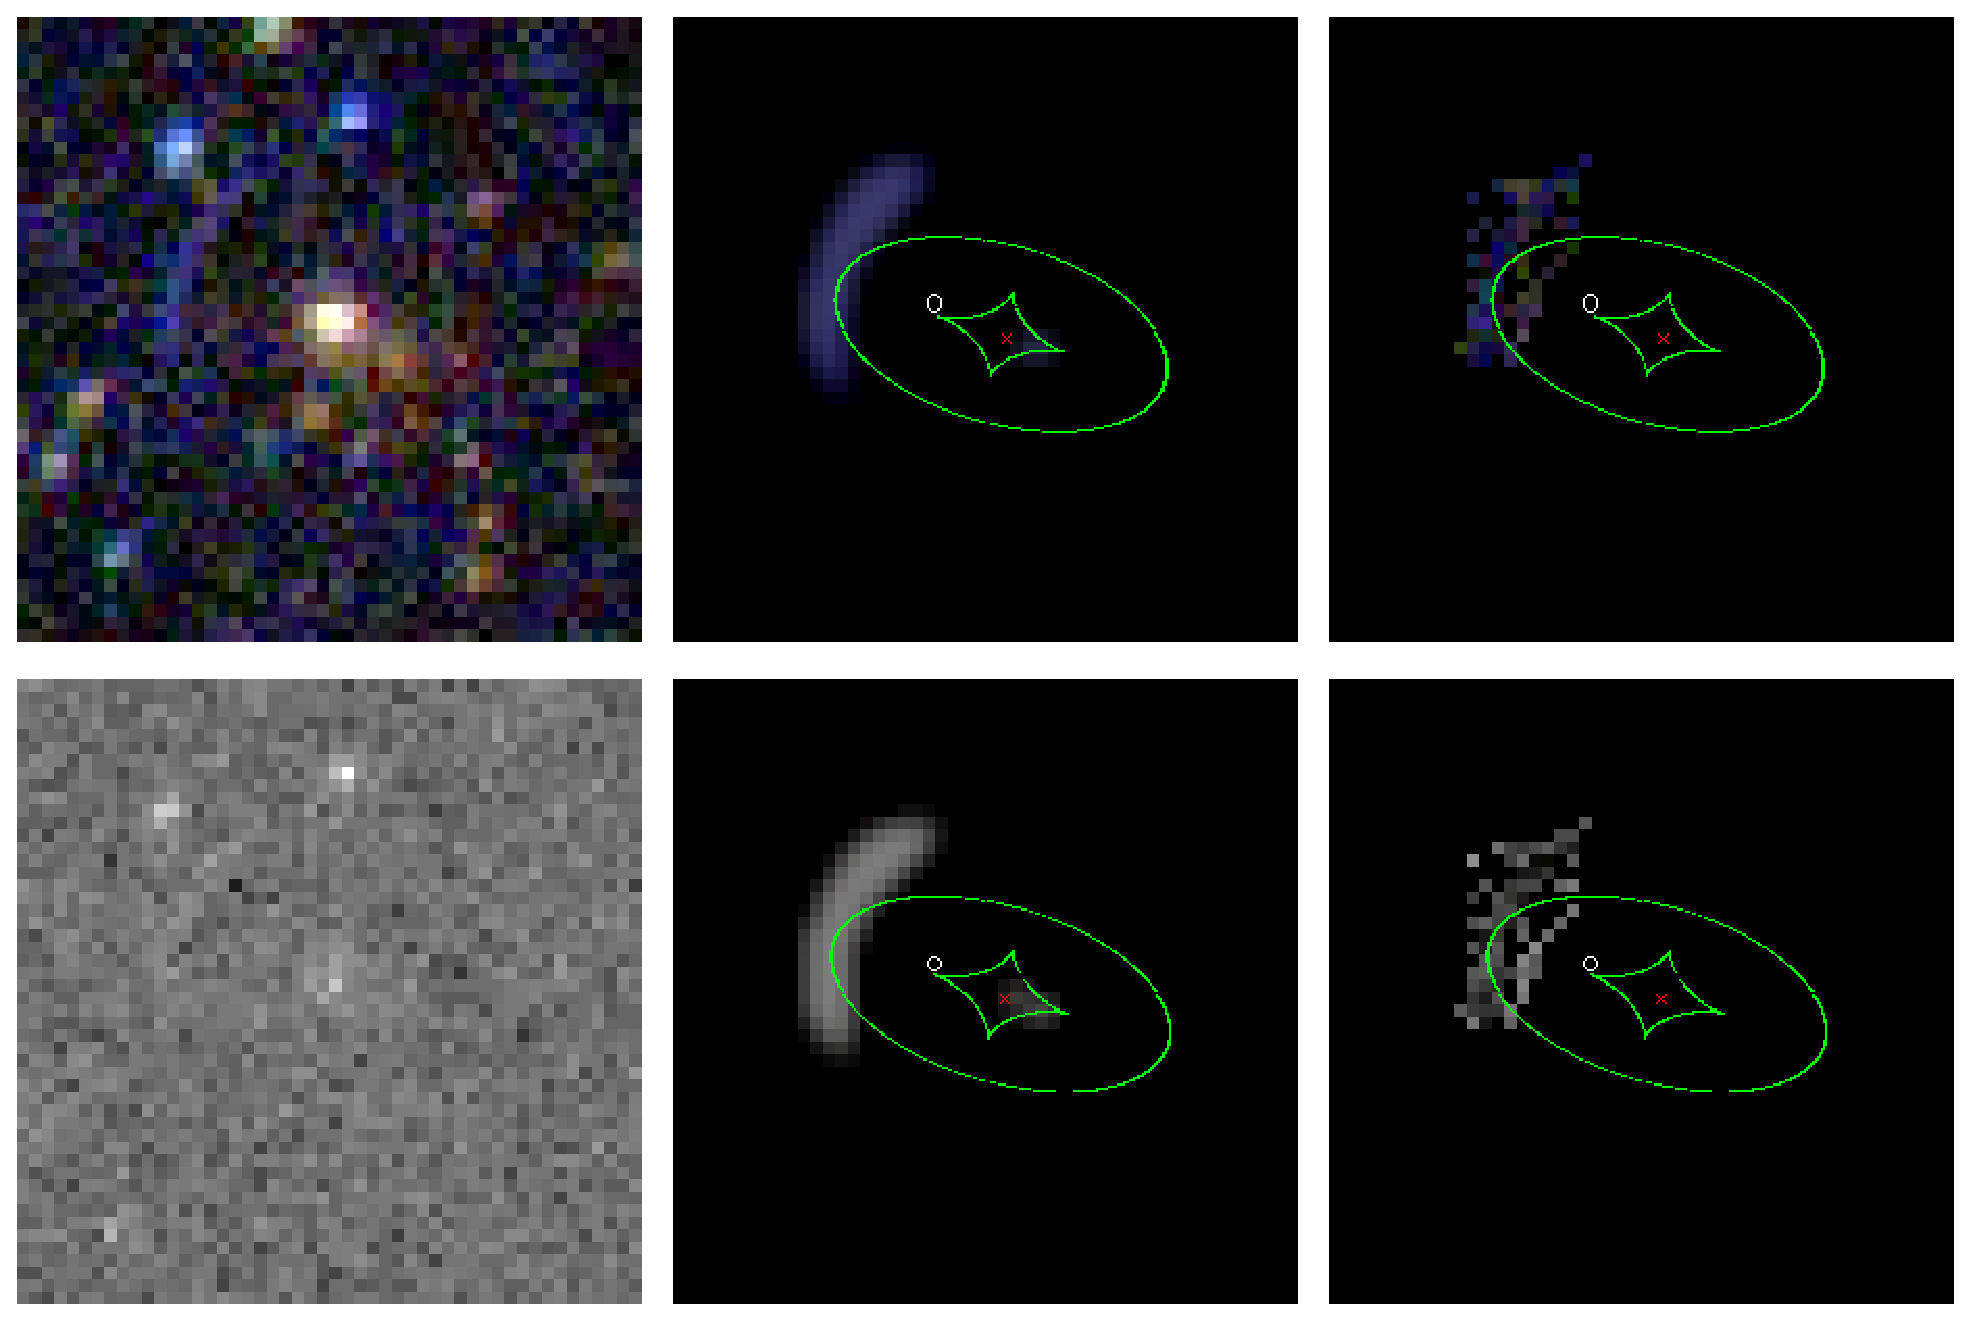
\includegraphics[width=\linewidth]{figs/8.eps}
	\caption{CSWA 8, see Figure~\ref{fig:cswa1} for caption.}
	\label{fig:cswa8}
\end{figure}
%%%%%%%%%%%%%%%%%%%%%%%%%%%%%%%%%%%%%%%%%%

This lens candidate is a massive galaxy cluster~\citep{OSK08}. We were able to
model this system using a single lens mass component elongated along the axis
between the  two brightest cluster galaxies, producing a long arc. The
counter-image is predicted to lie in the central part of the cluster, in amongst
the bright cluster member galaxies: higher resolution, deeper imaging would
allow this counter-image to be cleanly separated. Our model has the source being
magnified by a factor of $6\pm2$; the lens has Einstein radius 7.8~arcsec. 


% . . . . . . . . . . . . . . . . . . . . . . . . . . . . . . . . . . . .  .  

\subsubsection*{CSWA~9: SDSS\ J1227$+$1725}
\label{sec:results:indinotes:cswa9}

% {\bf CLASSIFICATION: B}

%%%%%%%%%%%%%%%%%%%%%%%%%%%%%%%%%%%%%%%%%%
\begin{figure}[!ht]
	\centering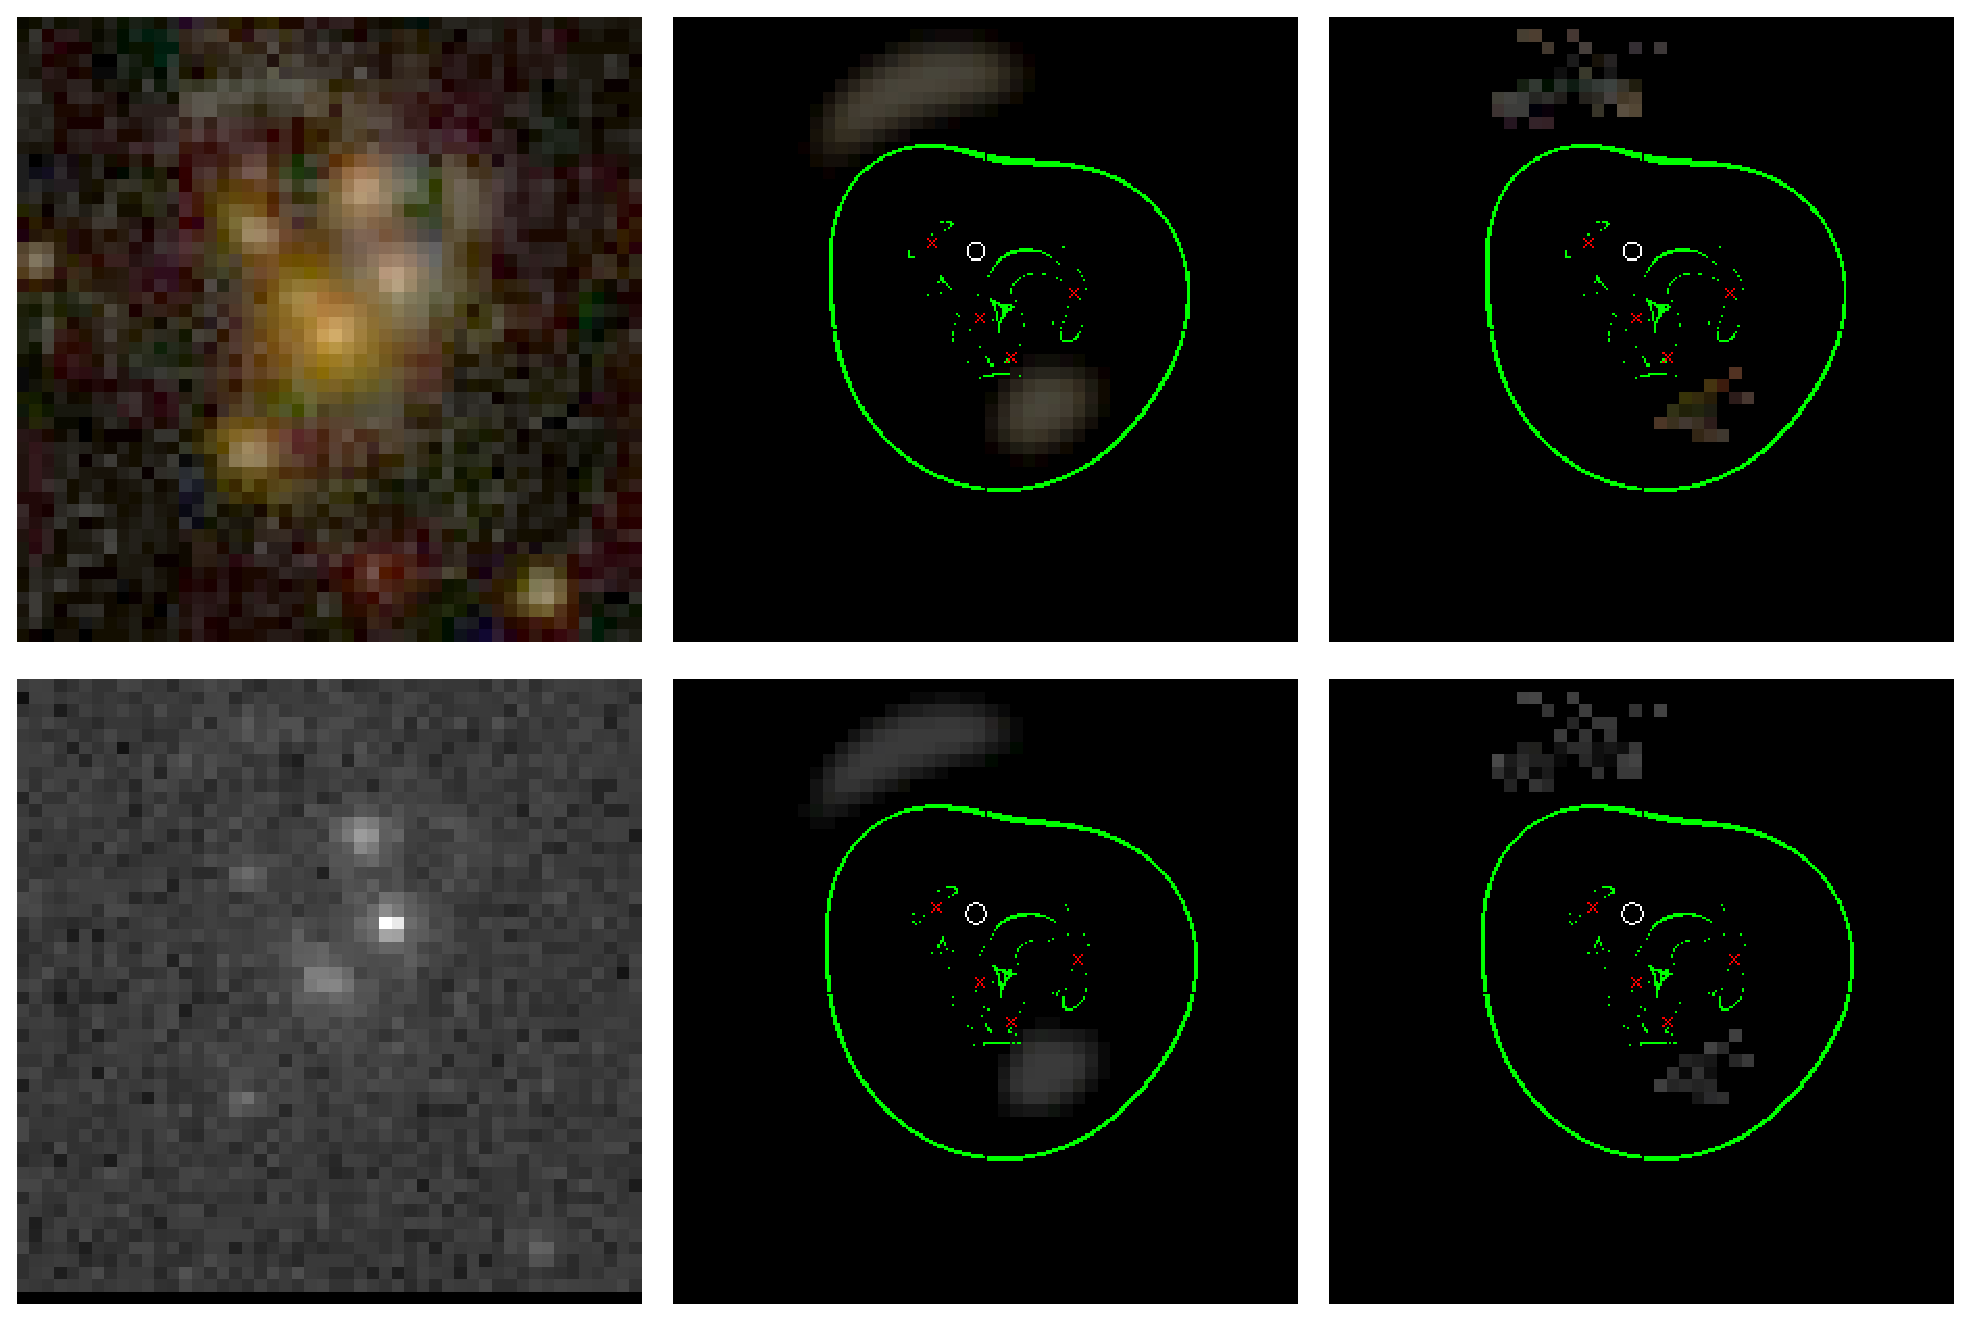
\includegraphics[width=\linewidth]{figs/9.eps}
	\caption{CSWA 9, see Figure~\ref{fig:cswa1} for caption.}
	\label{fig:cswa9}
\end{figure}

CSWA~9 is a cluster of galaxies; this lens candidate was modeled using two lens
components of comparable mass.  Our model successfully reproduces the Northern
arc, with a counter-image consistent with the faint emission just South of the
BCG. A second, shorter arc to the North-West, of comparable color to the
Northern arc, was not modelled: it may be singly imaged, or have a counter-image
buried in the cluster light (if it is indeed a second background source).

% . . . . . . . . . . . . . . . . . . . . . . . . . . . . . . . . . . . .  .  

\subsubsection*{CSWA~10: SDSS\ J2238$+$1319}
\label{sec:results:indinotes:cswa10}

% {\bf CLASSIFICATION: A}

%%%%%%%%%%%%%%%%%%%%%%%%%%%%%%%%%%%%%%%%%%
\begin{figure}[!ht]
	\centering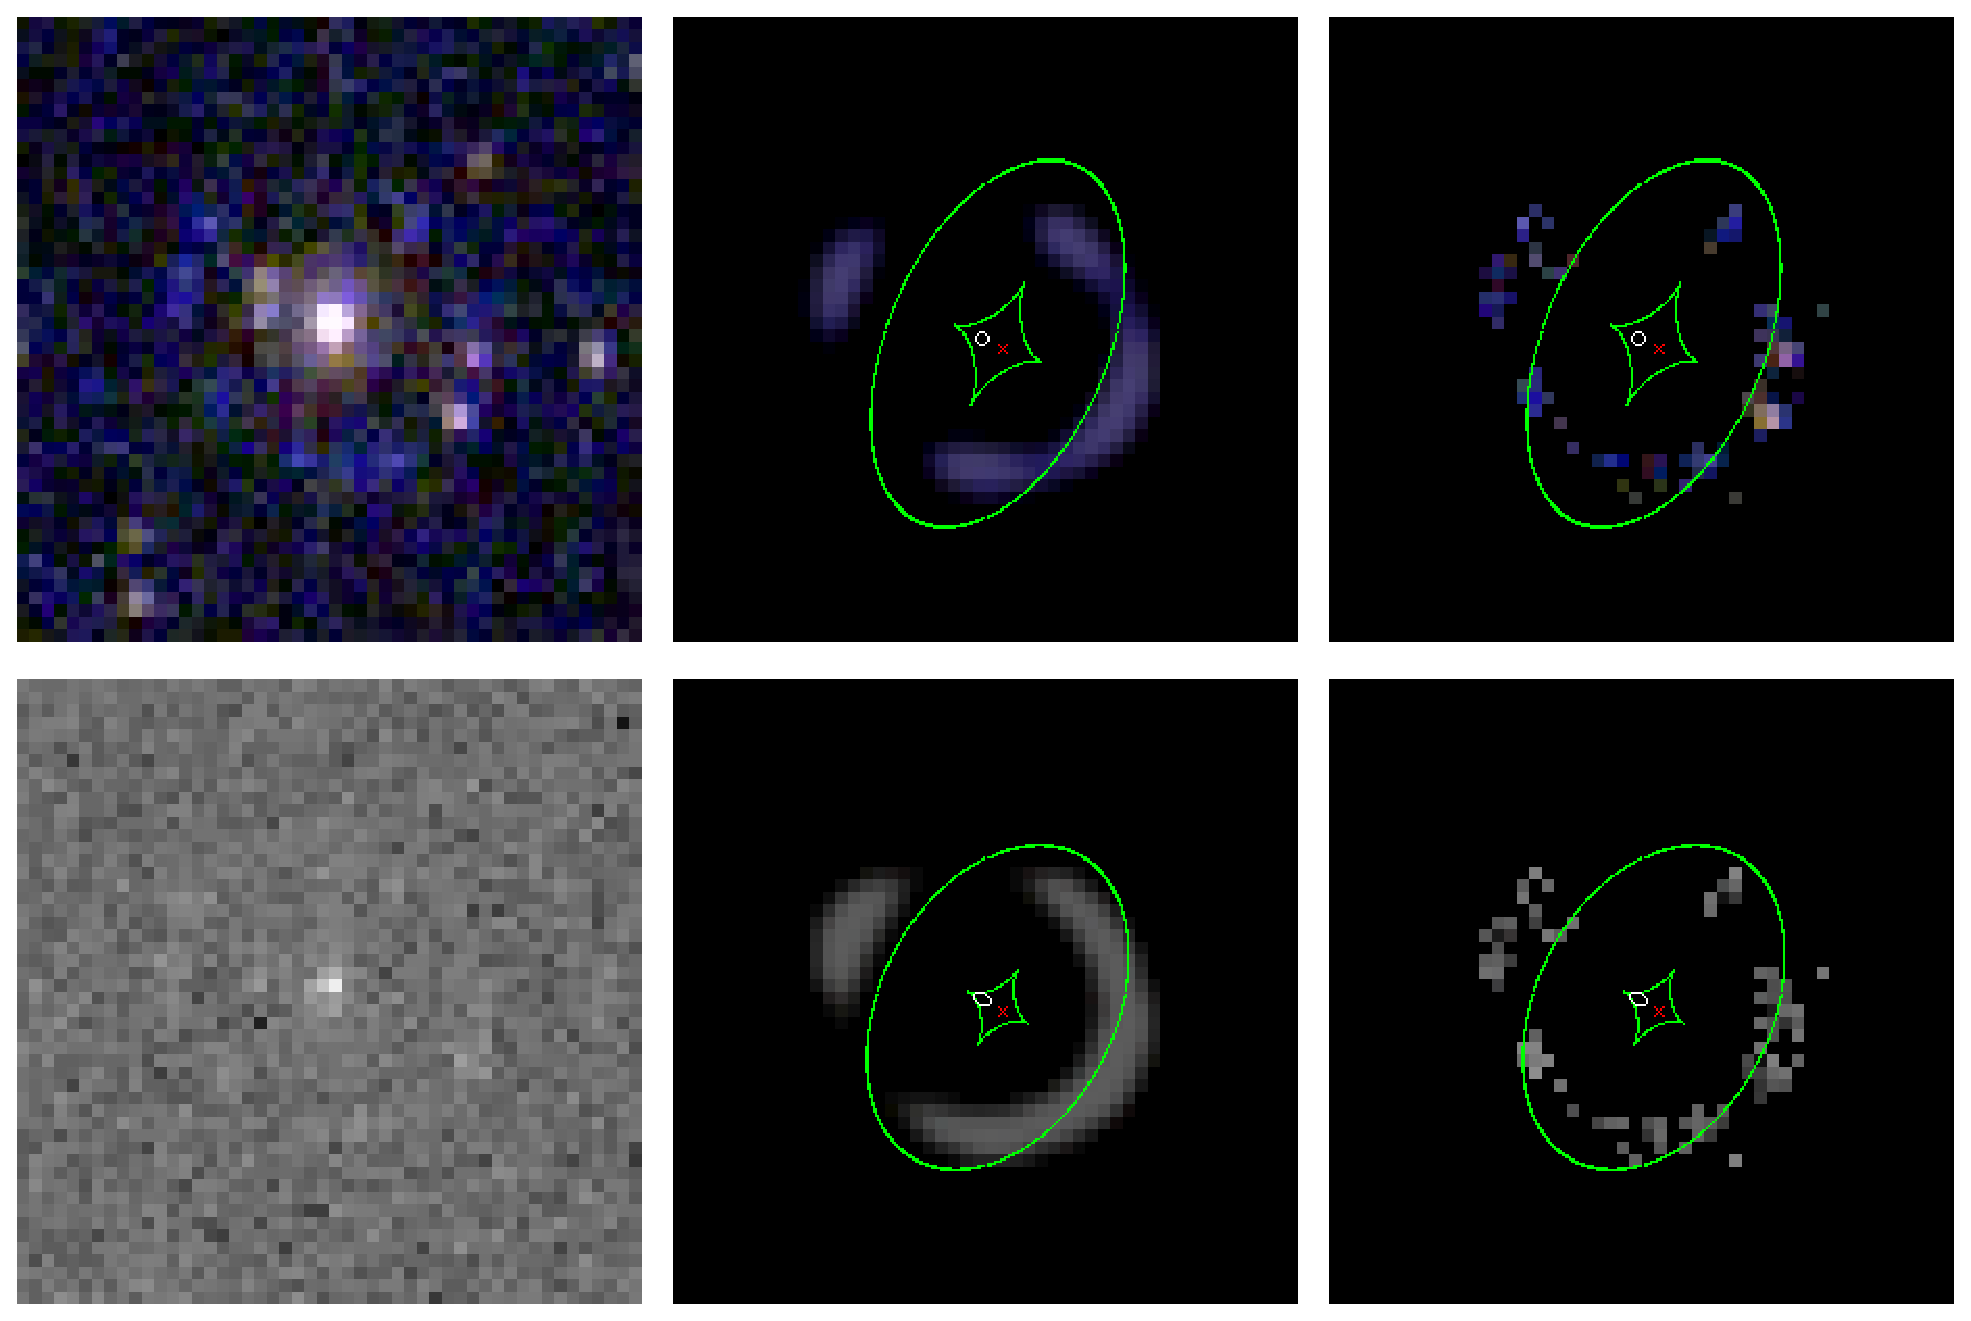
\includegraphics[width=\linewidth]{figs/10.eps}
	\caption{CSWA 10, see Figure~\ref{fig:cswa1} for caption.}
	\label{fig:cswa10}
\end{figure}
%%%%%%%%%%%%%%%%%%%%%%%%%%%%%%%%%%%%%%%%%%

This candidate is very similar to CSWA~1 in that it consists of three arcs,
forming a nearly complete, slightly oval-shaped ring. However, the arcs are
observed at quite low signal to noise in the SDSS imaging, and appear broken up
as a result. It is also possible that the source is multi-component in nature. 
We modeled this multiple-imaging  system using a single lens and a single
source, and were able to reproduce the basic image separation but not the
detailed morphology -- moreover, two satellite galaxies lie at the arc radius,
not detectably perturbing the arc morphology but contributing unlensed
brightness to the image. As a result the $\Omega$ value for this system is
relatively low (42\%). The model shown is not unique, in the sense that other
combinations of parameters give comparable fits -- the Einstein radius of the
lens is, however, quite robustly estimated at $9.0\pm0.1$~arcsec.


% . . . . . . . . . . . . . . . . . . . . . . . . . . . . . . . . . . . .  .  

\subsubsection*{CSWA~11: SDSS\ J0800$+$0812}
\label{sec:results:indinotes:cswa11}

% % {\bf CLASSIFICATION: B}

%%%%%%%%%%%%%%%%%%%%%%%%%%%%%%%%%%%%%%%%%%
\begin{figure}[!ht]
	\centering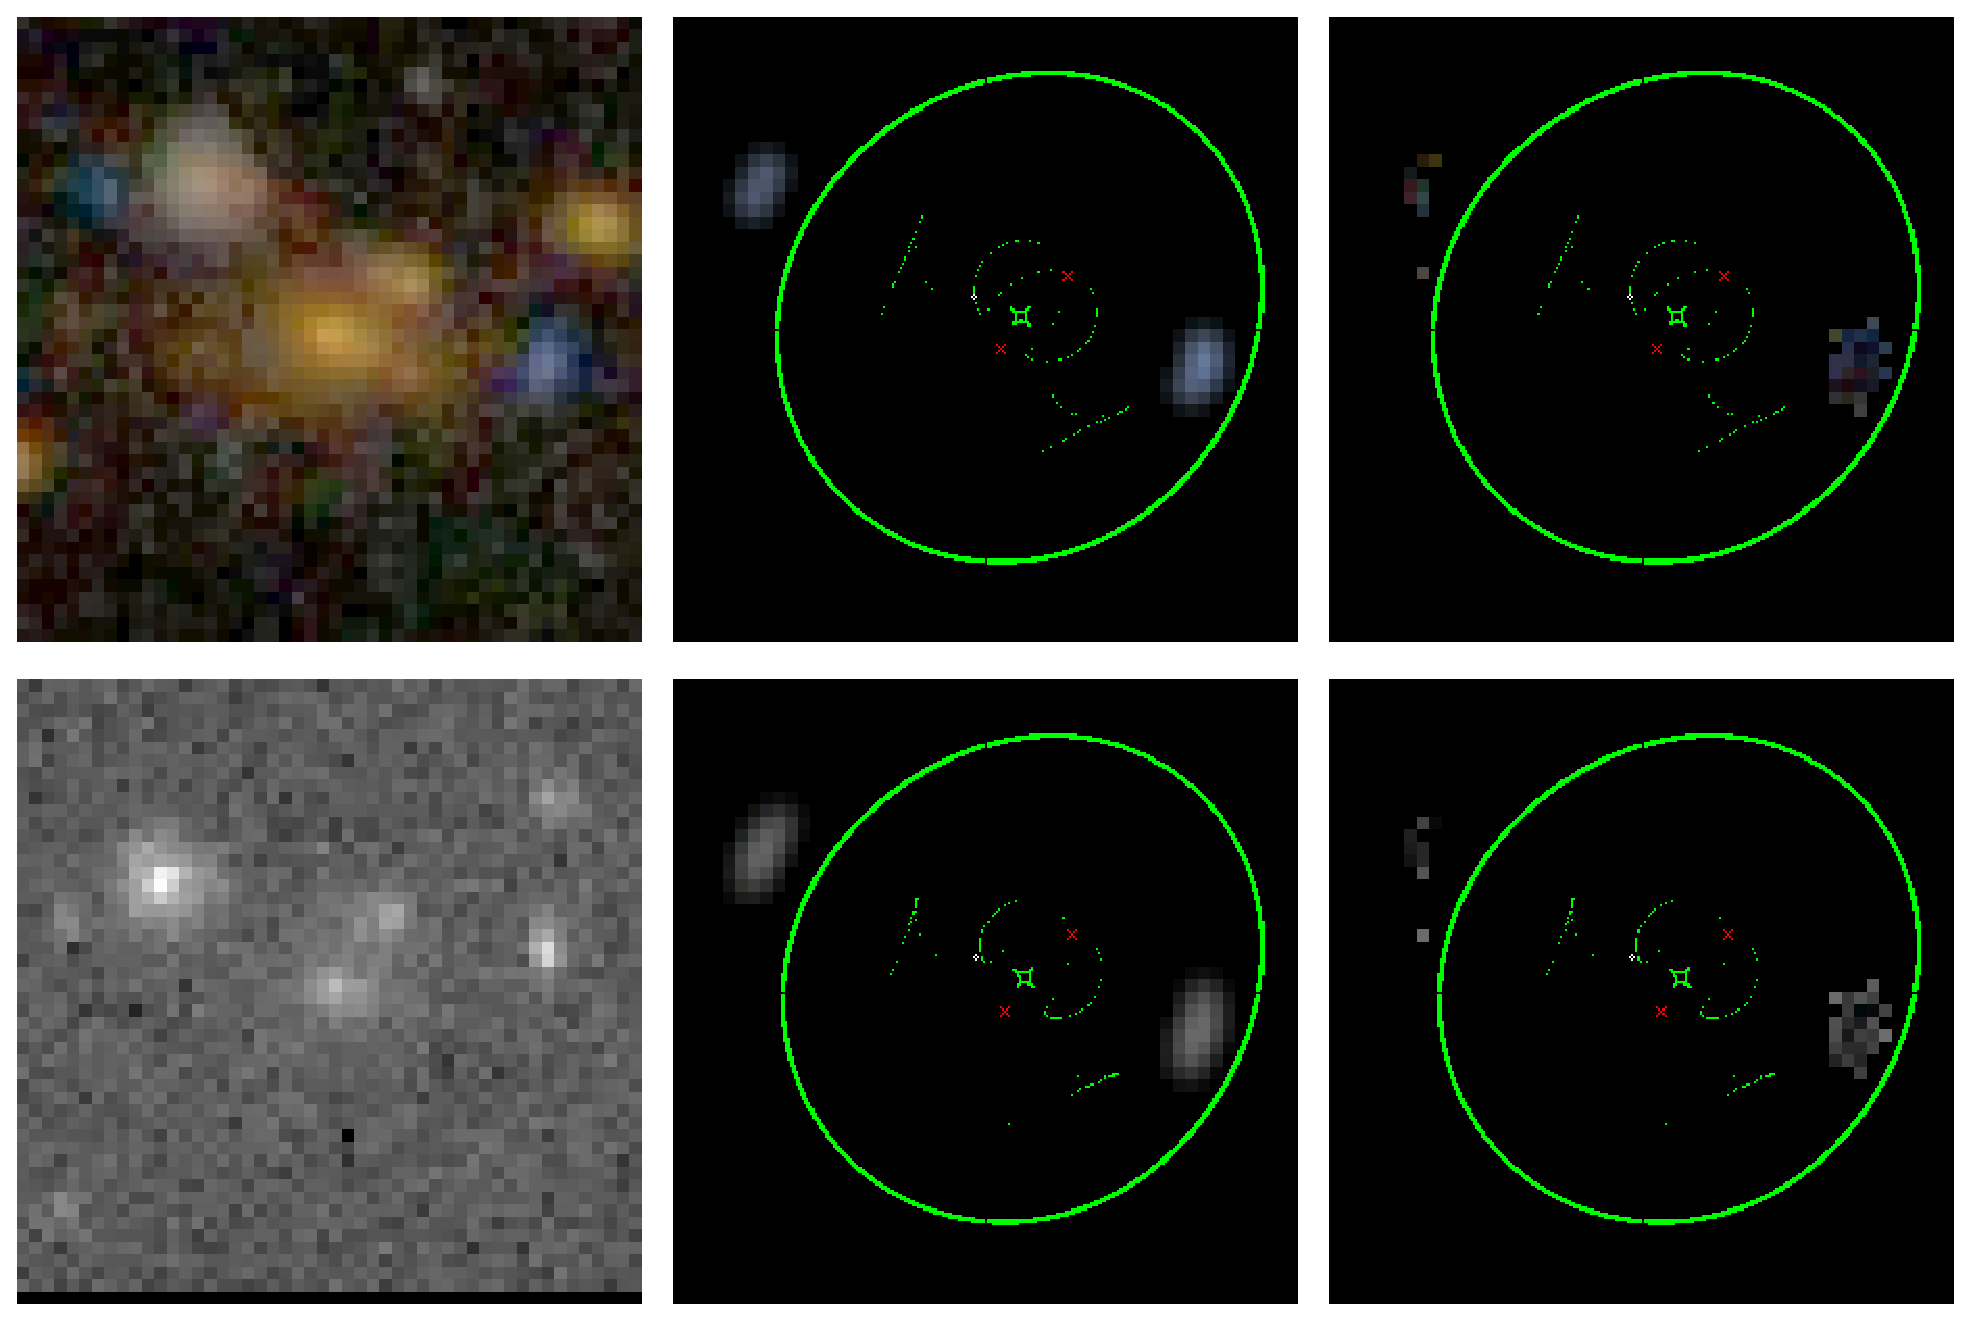
\includegraphics[width=\linewidth]{figs/11.eps}
	\caption{CSWA 11, see Figure~\ref{fig:cswa1} for caption.}
	\label{fig:cswa11}
\end{figure}
%%%%%%%%%%%%%%%%%%%%%%%%%%%%%%%%%%%%%%%%%%

CSWA~11, like CSWA~10, is a small cluster of galaxies.  The candidate arcs are
bright blue objects to the East and West of the cluster center.  With two lens
galaxies and a single source, we were able to reproduce the positions, and
relative brightnesses, of the two small blue images quite naturally. However,
the predicted arcs were significantly more elongated tangentially than the
observed images: this suggests that either the source is smaller than we can
model with \theapplet, or we are seeing two unlensed, or weakly lensed, blue
objects. The Western blue object may be the bright image of a double, with the
counter-image just East of the BCG -- such a model would also require a small
source to avoid over-predicting the tangential smearing.

The North-Eastern pink-ish object is  likely a foreground galaxy which does not
contribute as strongly  to the lensing taking place. If it were in the same
plane as the lensing galaxies, it would tend to cause the North-Eastern image to
elongate unless its Einstein radius was under $0.4"$.


% . . . . . . . . . . . . . . . . . . . . . . . . . . . . . . . . . . . .  .  

\subsubsection*{CSWA~12: SDSS\ J1133$+$5008}
\label{sec:results:indinotes:cswa12}

% {\bf CLASSIFICATION: A}

%%%%%%%%%%%%%%%%%%%%%%%%%%%%%%%%%%%%%%%%%%
\begin{figure}[!ht]
	\centering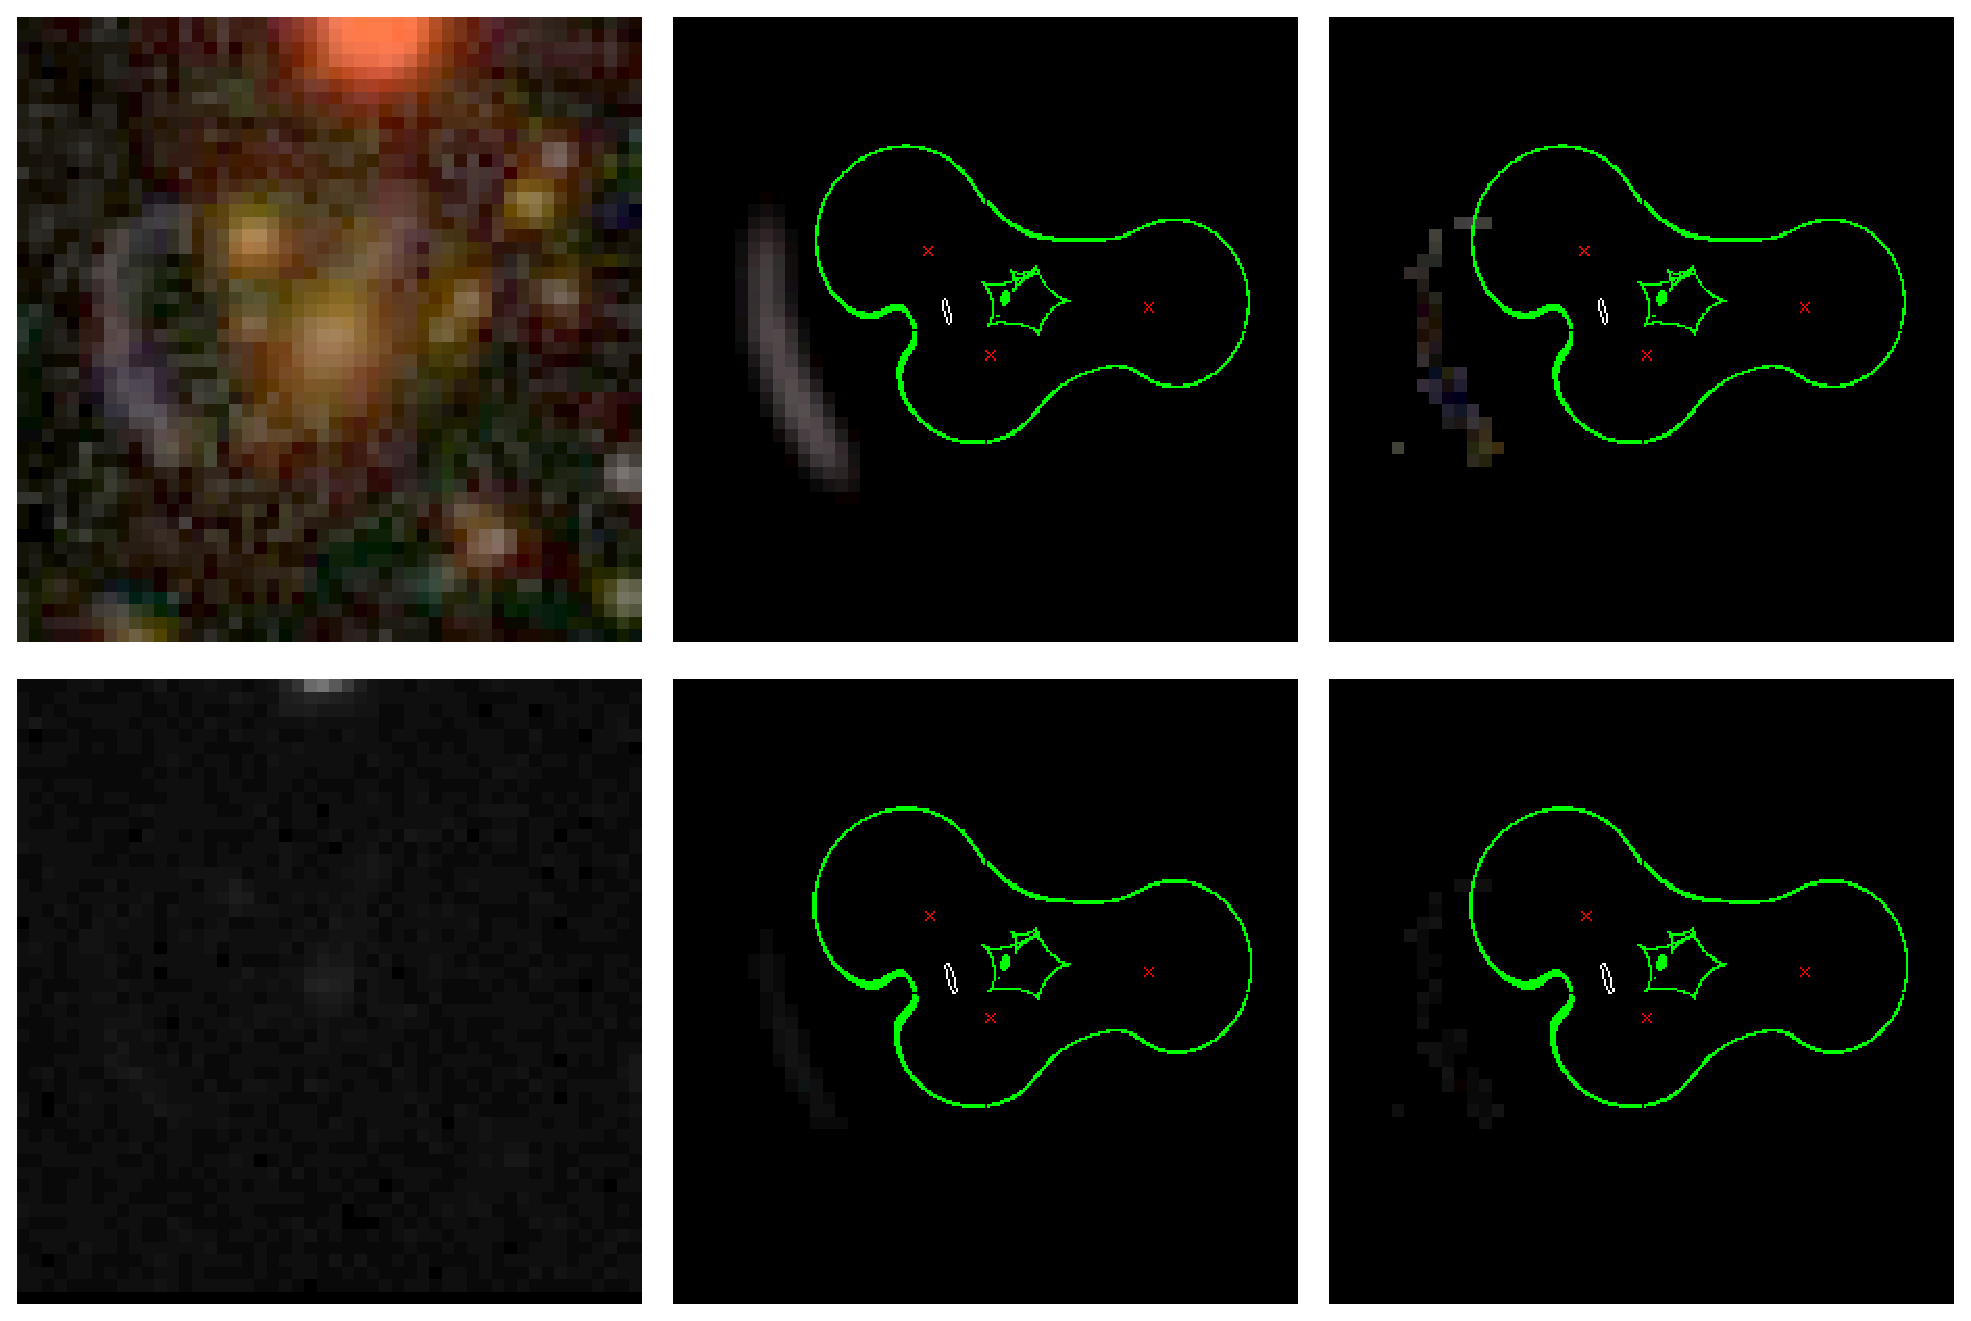
\includegraphics[width=\linewidth]{figs/12.eps}
	\caption{CSWA 12, see Figure~\ref{fig:cswa1} for caption.}
	\label{fig:cswa12}
\end{figure}
%%%%%%%%%%%%%%%%%%%%%%%%%%%%%%%%%%%%%%%%%%

This small, compact galaxy cluster was modeled using three lens mass components
of approximately equal mass, centered on the three most central lens galaxies.
This led to some complex caustic structures in the source plane. We were able to
produce an arc of approximately the right length and curvature to match the
observed feature. Its counter-image is predicted to lie in the central part of
the cluster, in amongst the lens galaxies. Its predicted position does not quite
match a faint feature of the required matching color, but is close.  Note that
the counter-images have been masked out in the residual image, an unavoidable
consequence of masking the lens galaxies. Overall, the residual image has very
few features in it.


% . . . . . . . . . . . . . . . . . . . . . . . . . . . . . . . . . . . .  .  

\subsubsection*{CSWA~13: SDSS\ J1237$+$5533}
\label{sec:results:indinotes:cswa13}

% {\bf CLASSIFICATION: B}

%%%%%%%%%%%%%%%%%%%%%%%%%%%%%%%%%%%%%%%%%%
\begin{figure}[!ht]
	\centering\includegraphics[width=\linewidth]{figs/13.eps}
  \caption{CSWA 13, showing models with one source (top row) and 2 sources
  (bottom row). Otherwise, see Figure~\ref{fig:cswa1} for caption.}
  \label{fig:cswa13}
\end{figure}
%%%%%%%%%%%%%%%%%%%%%%%%%%%%%%%%%%%%%%%%%%

This lens candidate, like CSWA~7, can be modeled using a single source and a
highly elliptical lens, or using two sources and a lens with lower ellipticity.
We show both of these models in Figure~\ref{fig:cswa13}. As in CSWA~7, the
Einstein radius for the two models are very similar.

This system is so similar to CSWA~7 that much of the same discussion of that
object holds here: although the single-source model has a faint residual image,
the circular light distribution of the lens does not indicate the highly
elliptical lens that is required by this model. However, the dual-source model
predicts a prominent counter-image, which does not appear in the astronomical
image. The single source model fits the data somewhat better ($\Omega = 86\%$
compared to 71\%). Not shown is a third model, with two sources neither of which
is multiply-imaged -- again, the high brightness of the arcs argues for them
being highly magnified, but the evidence for multiple-imaging is not clear-cut. 


% . . . . . . . . . . . . . . . . . . . . . . . . . . . . . . . . . . . .  .  

\subsubsection*{CSWA~14: SDSS\ J1723$+$3411}
\label{sec:results:indinotes:cswa14}

% {\bf CLASSIFICATION: A}

%%%%%%%%%%%%%%%%%%%%%%%%%%%%%%%%%%%%%%%%%%
\begin{figure}[!ht]
	\centering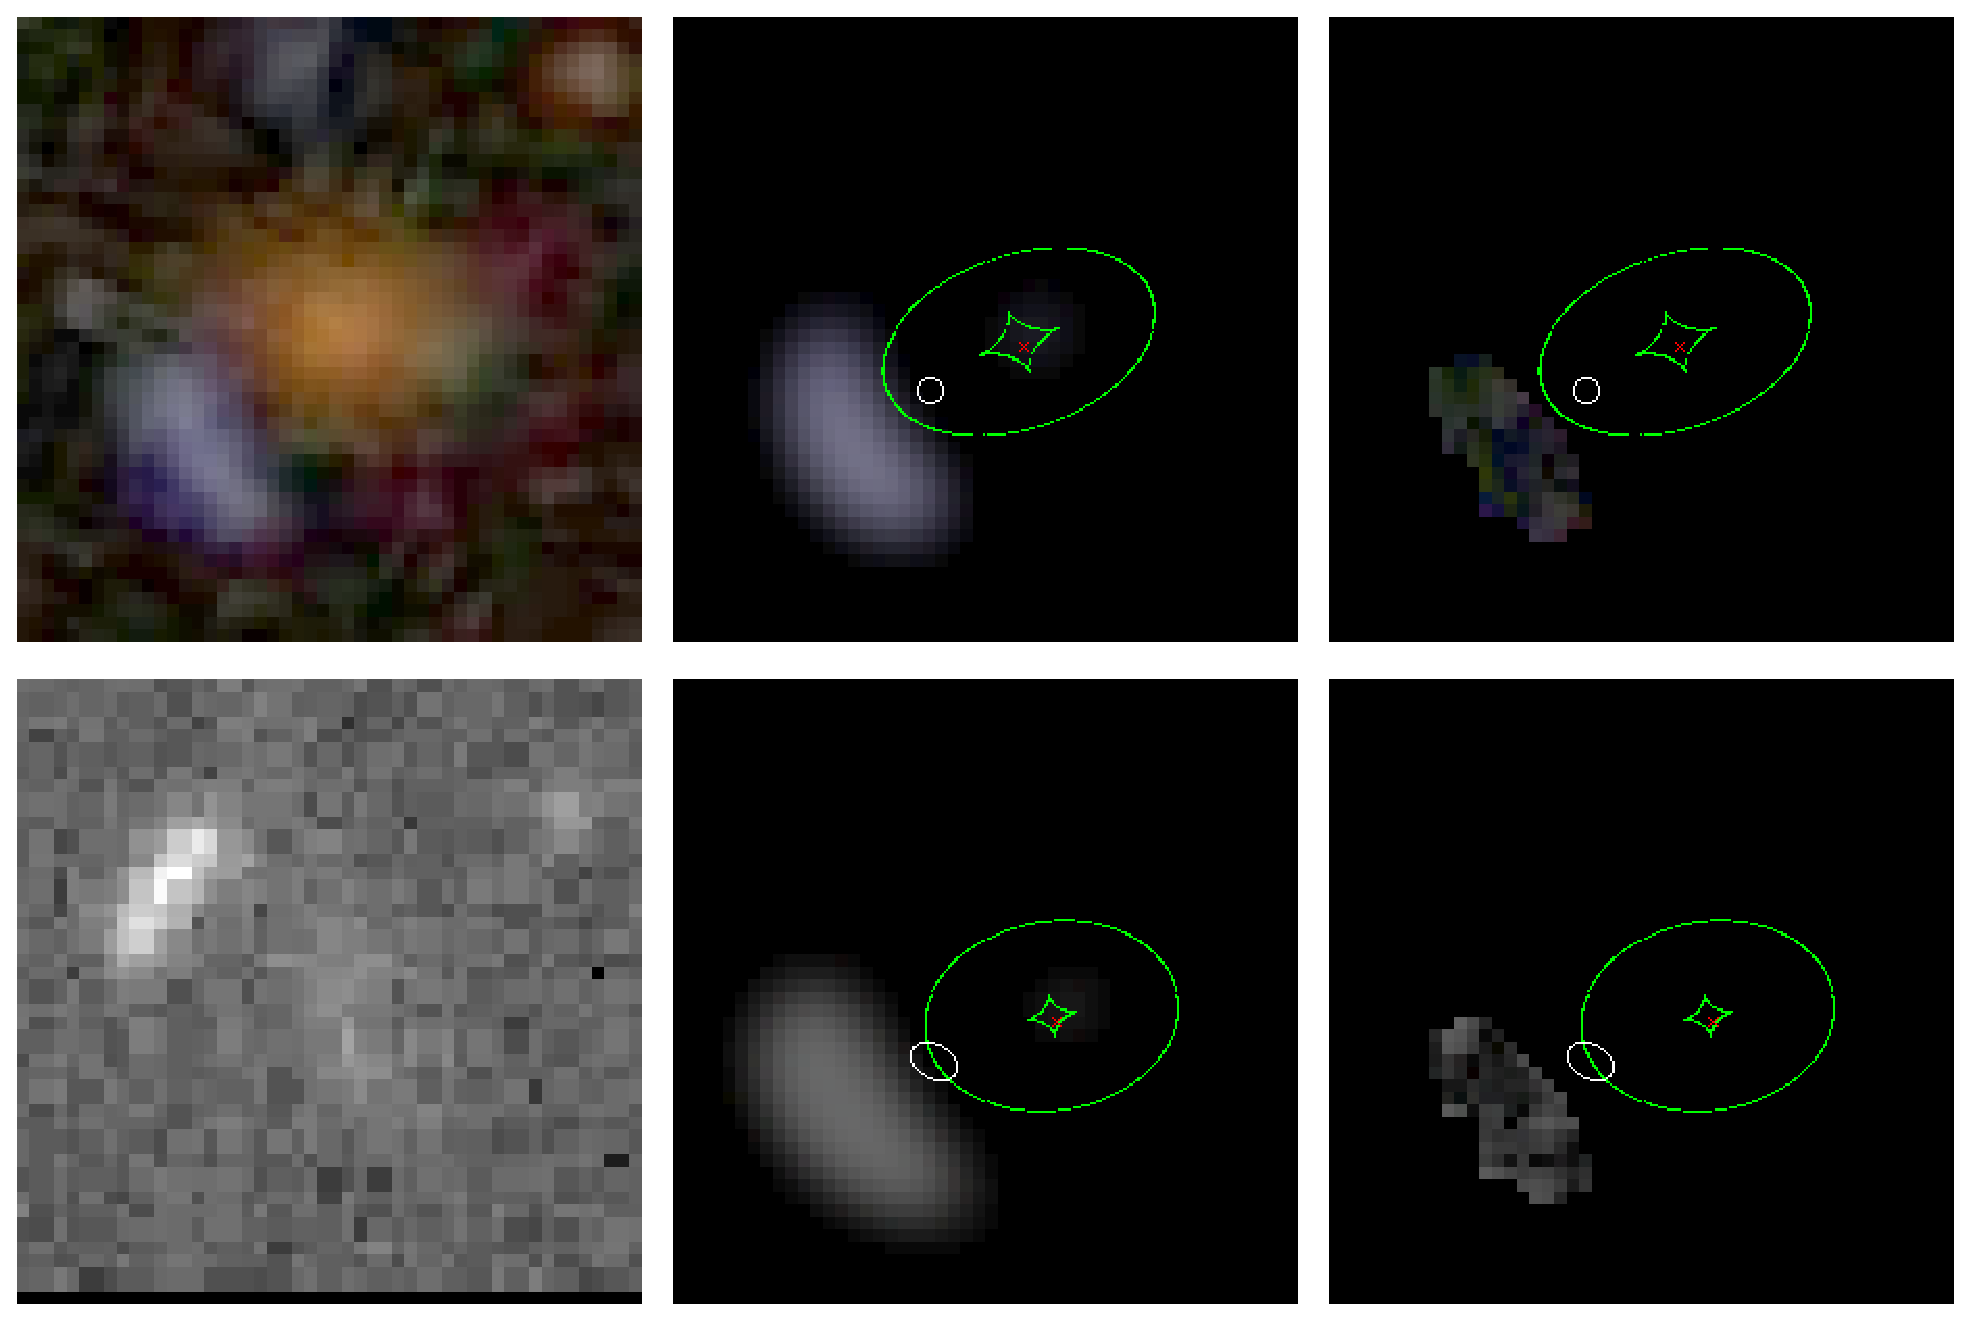
\includegraphics[width=\linewidth]{figs/14.eps}
	\caption{CSWA 14, see Figure~\ref{fig:cswa1} for caption.}
	\label{fig:cswa14}
\end{figure}
%%%%%%%%%%%%%%%%%%%%%%%%%%%%%%%%%%%%%%%%%%

CSWA~14 is also one of the SDSS bright arc candidates followed up by
\citet{Kub++10}, who measured spectroscopic redshifts for both the main lens
galaxy and the straight blue arc. This lens candidate is easily modeled using a
single source and a single lens. Although our model predicts a counter-image not
present in the astronomical image, it is very faint. The predicted arc is also
rather more curved than the observed one: it is the high brightness of the blue
feature that argues for the source being highly magnified and likely to be
strongly lensed. Our model has Einstein radius $3.3\pm0.1$~arcsec, somewhat
lower than the rough estimate made by \citet{Kub++10} of $\simeq 4.7$~arcsec.


% . . . . . . . . . . . . . . . . . . . . . . . . . . . . . . . . . . . .  .  

\subsubsection*{CSWA~15: SDSS\ J1008$+$1937}
\label{sec:results:indinotes:cswa15}

% {\bf CLASSIFICATION: B}

%%%%%%%%%%%%%%%%%%%%%%%%%%%%%%%%%%%%%%%%%%
\begin{figure}[!ht]
	\centering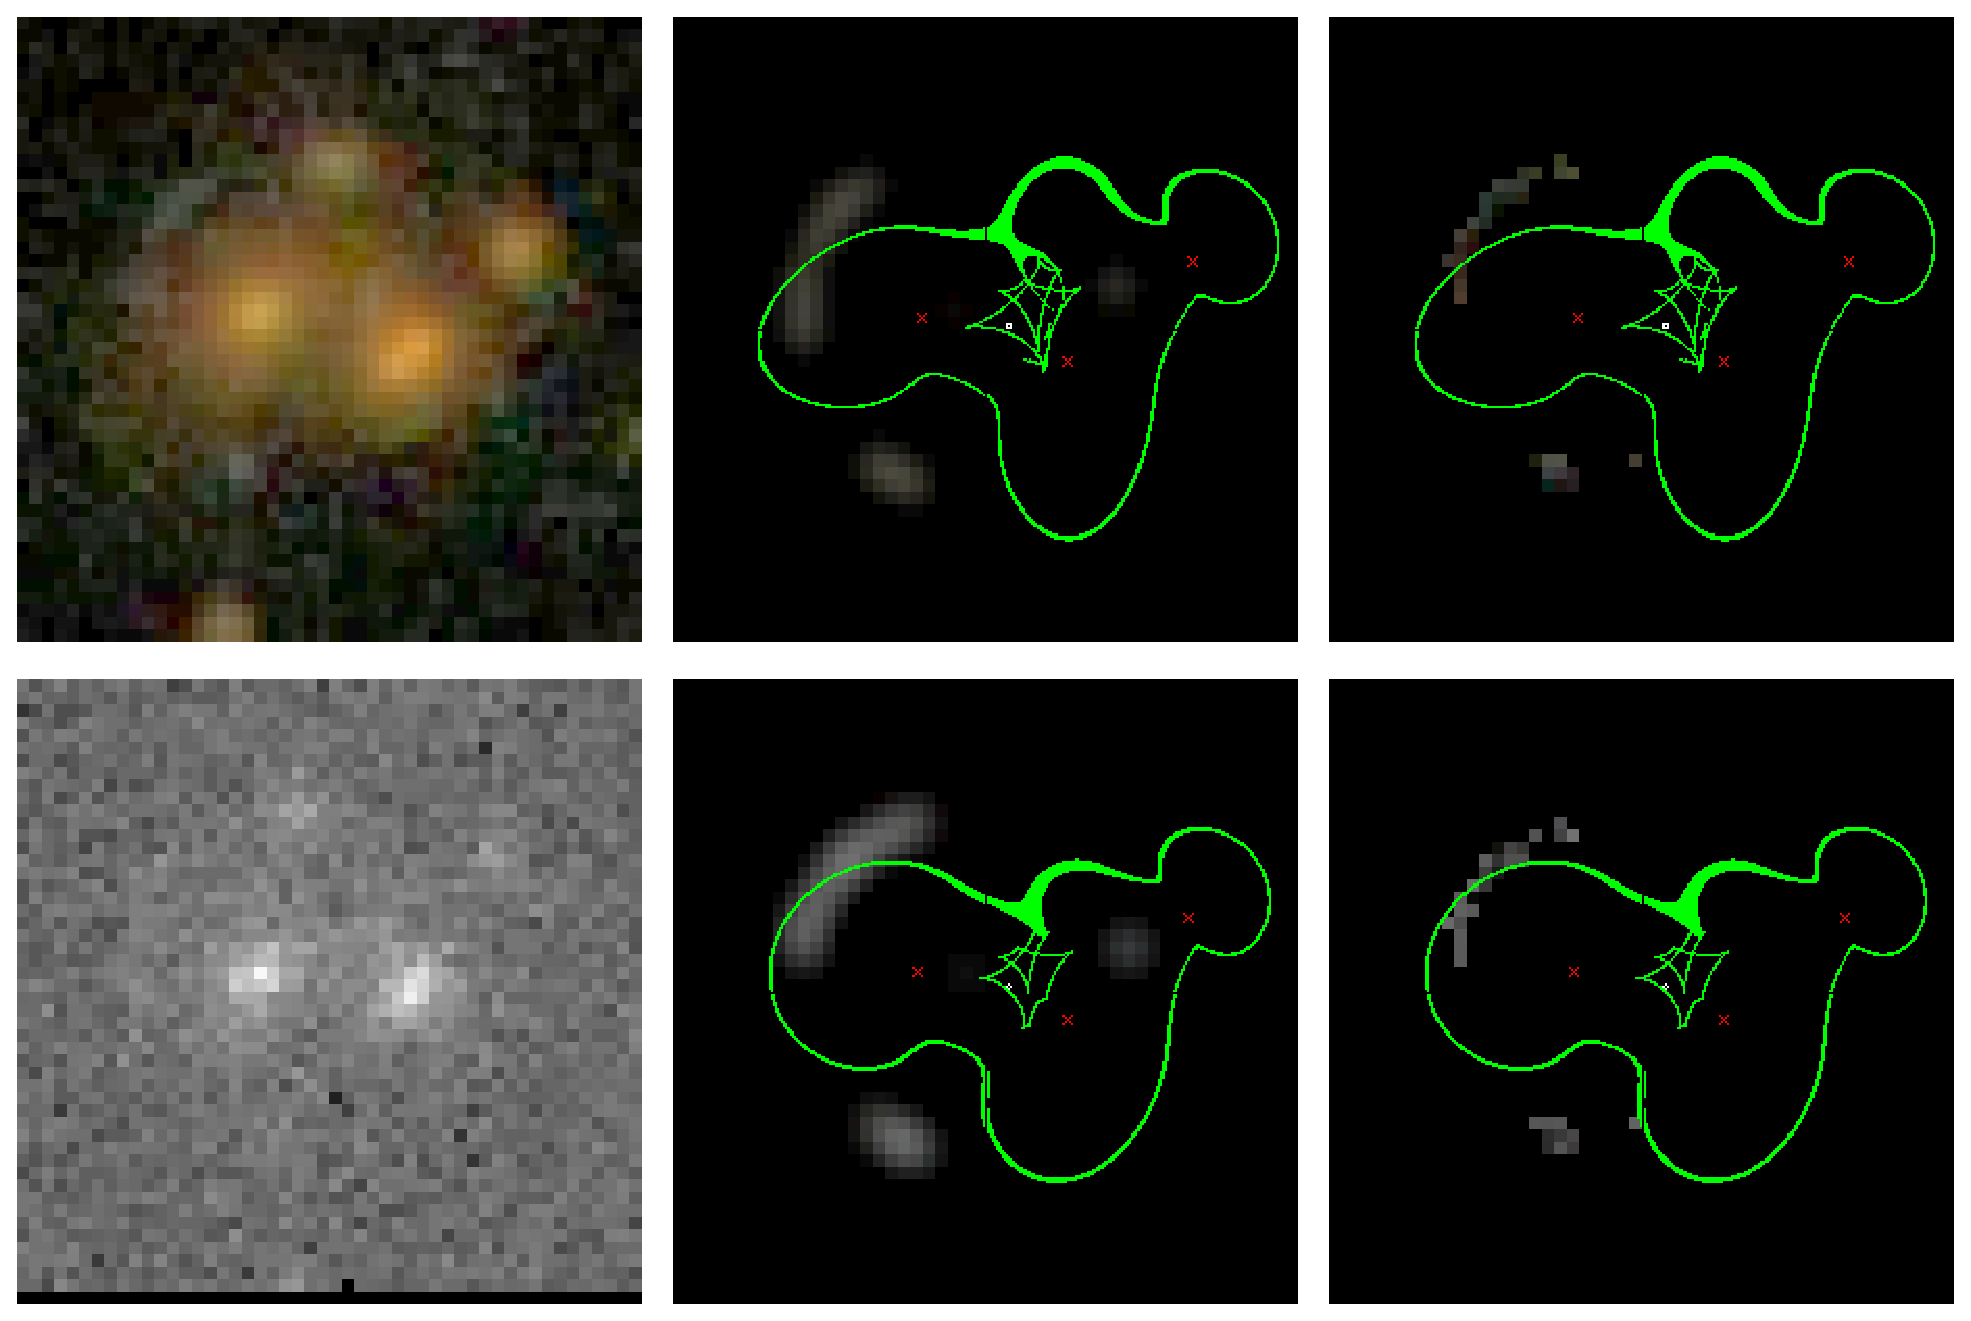
\includegraphics[width=\linewidth]{figs/15.eps}
	\caption{CSWA 15, see Figure~\ref{fig:cswa1} for caption.}
	\label{fig:cswa15}
\end{figure}
%%%%%%%%%%%%%%%%%%%%%%%%%%%%%%%%%%%%%%%%%%

CSWA~15 is another compact cluster of galaxies, with two central LRGs of
comparable brightness, with two satellites to the North and West.  The candidate
lensed feature is a short, tangentially aligned, curved arc to the North-East of
the Eastern main LRG; a small object of comparable colour and surface brighness
lies to the South as a candidate counter-image.  Modeling the system with three
lens components and a single source, we are able to match the positions of the
two lensed features, but slightly over predict their elongation. We also predict
a faint counter-image (the fourth image of the quad) to the West, where it could
lie obscured by the cluster light. 


% . . . . . . . . . . . . . . . . . . . . . . . . . . . . . . . . . . . .  .  

\subsubsection*{CSWA~16: SDSS\ J1111$+$5308}
\label{sec:results:indinotes:cswa16}

% {\bf CLASSIFICATION: C}

%%%%%%%%%%%%%%%%%%%%%%%%%%%%%%%%%%%%%%%%%%
\begin{figure}[!ht]
	\centering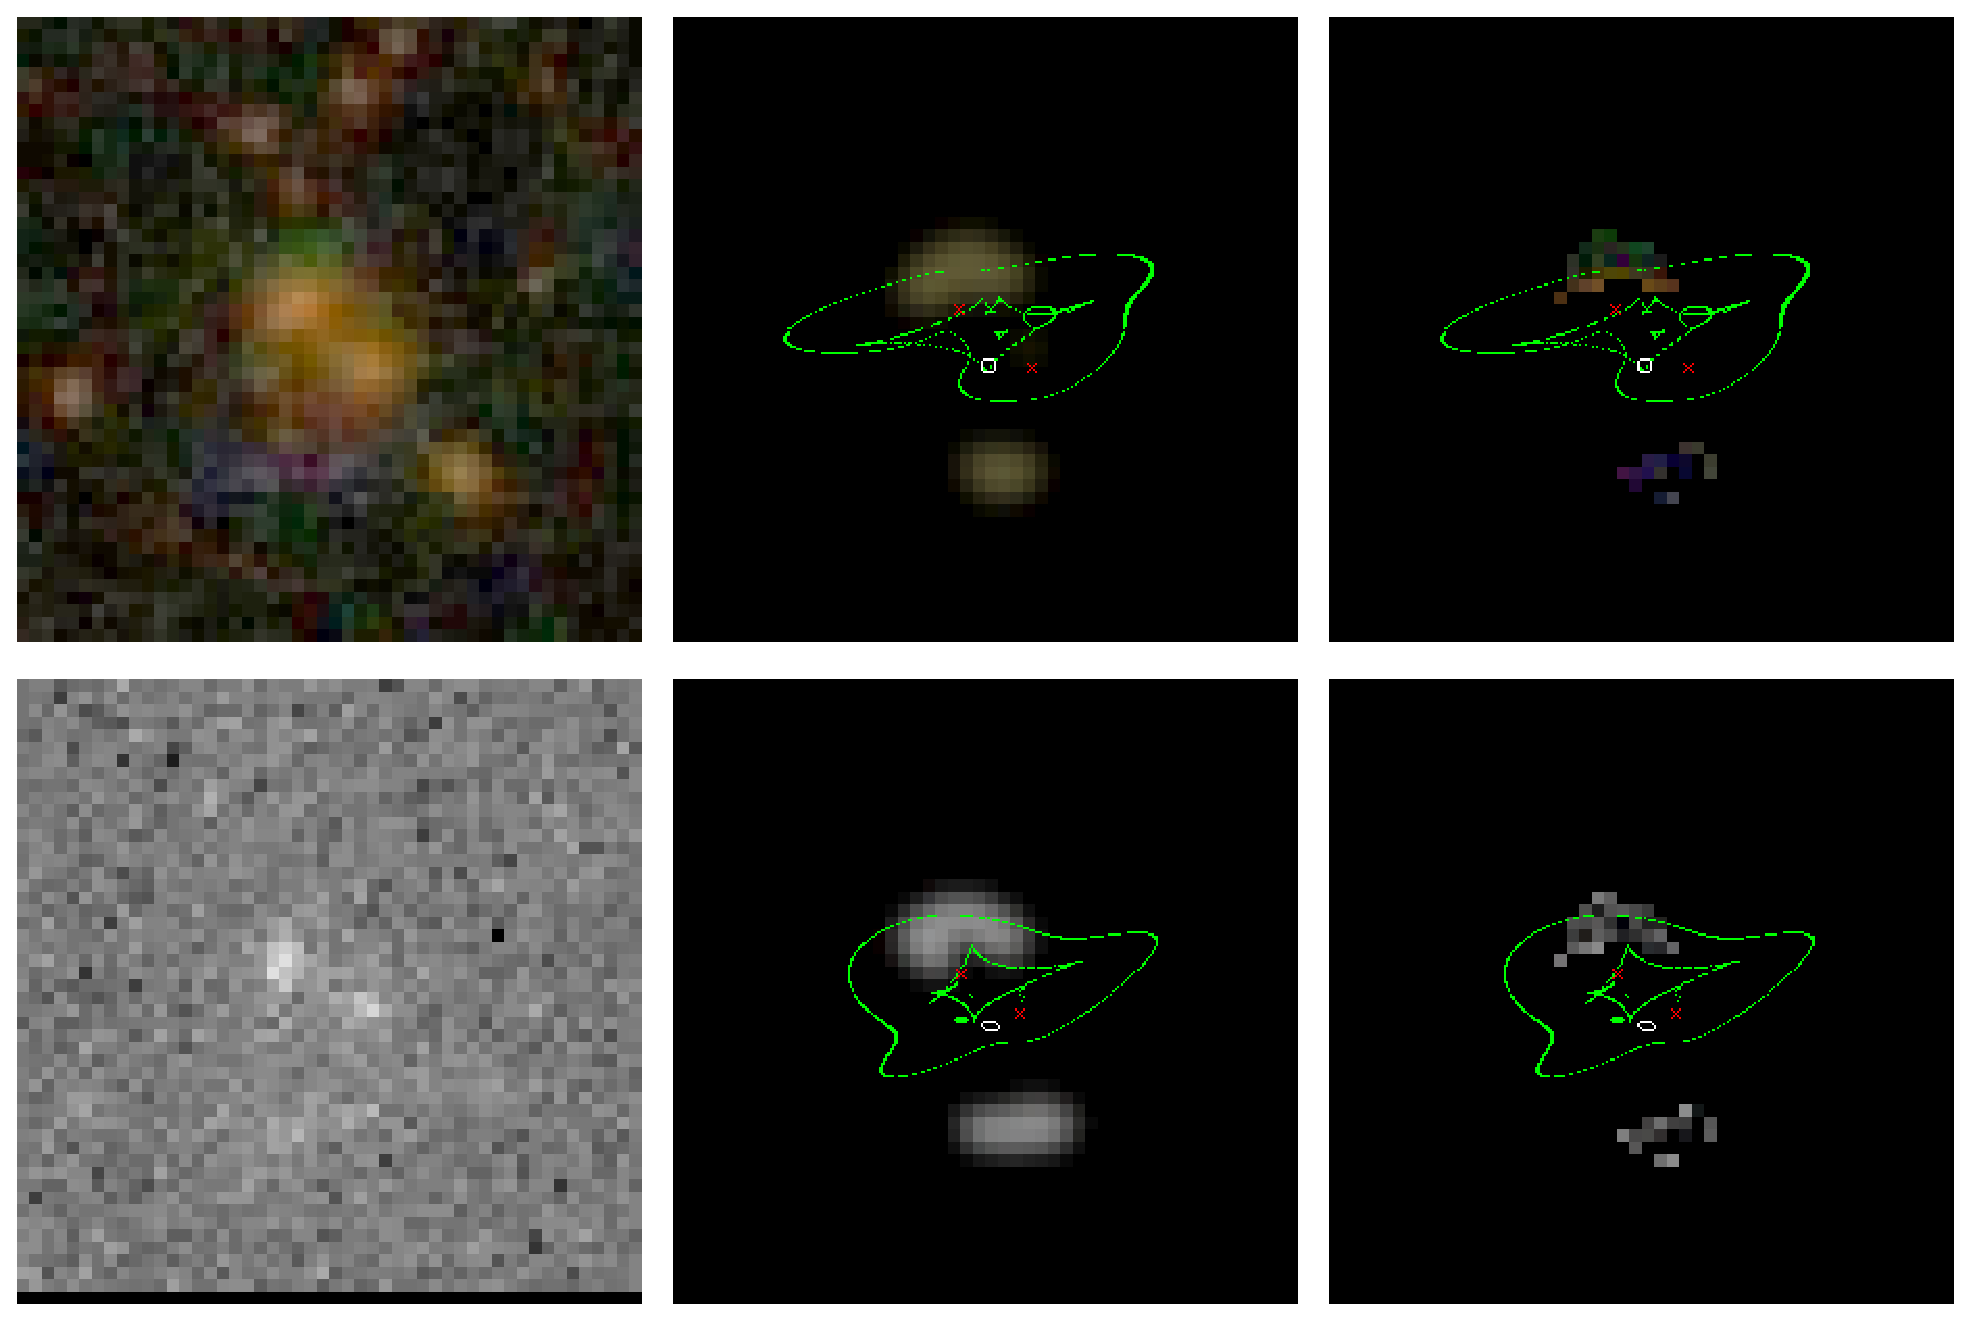
\includegraphics[width=\linewidth]{figs/16.eps}
	\caption{CSWA 16, see Figure~\ref{fig:cswa1} for caption.}
	\label{fig:cswa16}
\end{figure}
%%%%%%%%%%%%%%%%%%%%%%%%%%%%%%%%%%%%%%%%%%

This candidate lens is dominated by a close pair of bright LRGs aligned
North-East -- South-West, with a further satellite to the South-West. The
candidate lensed feature is a pair of blue objects arranged in a curved shape
but not aligned tangentially to the LRG pair. It is possible that the green
light to the North of the lens is the counter-image to this offset, misaligned
arc. Modeling the system with two lens galaxies and a single source, we are only
able to reproduce the arc position very roughly: the corresponding  predicted
counter-image is in approximately the right place, but rather too bright. Adding
mass at the position of the satellite galaxy does not improve the model -- in
fact it makes it harder to predict the candidate arc positions.


% . . . . . . . . . . . . . . . . . . . . . . . . . . . . . . . . . . . .  .  

\subsubsection*{CSWA~17: SDSS\ J1138$+$2754}
\label{sec:results:indinotes:cswa17}

% {\bf CLASSIFICATION: B}

%%%%%%%%%%%%%%%%%%%%%%%%%%%%%%%%%%%%%%%%%%
\begin{figure}[!ht]
	\centering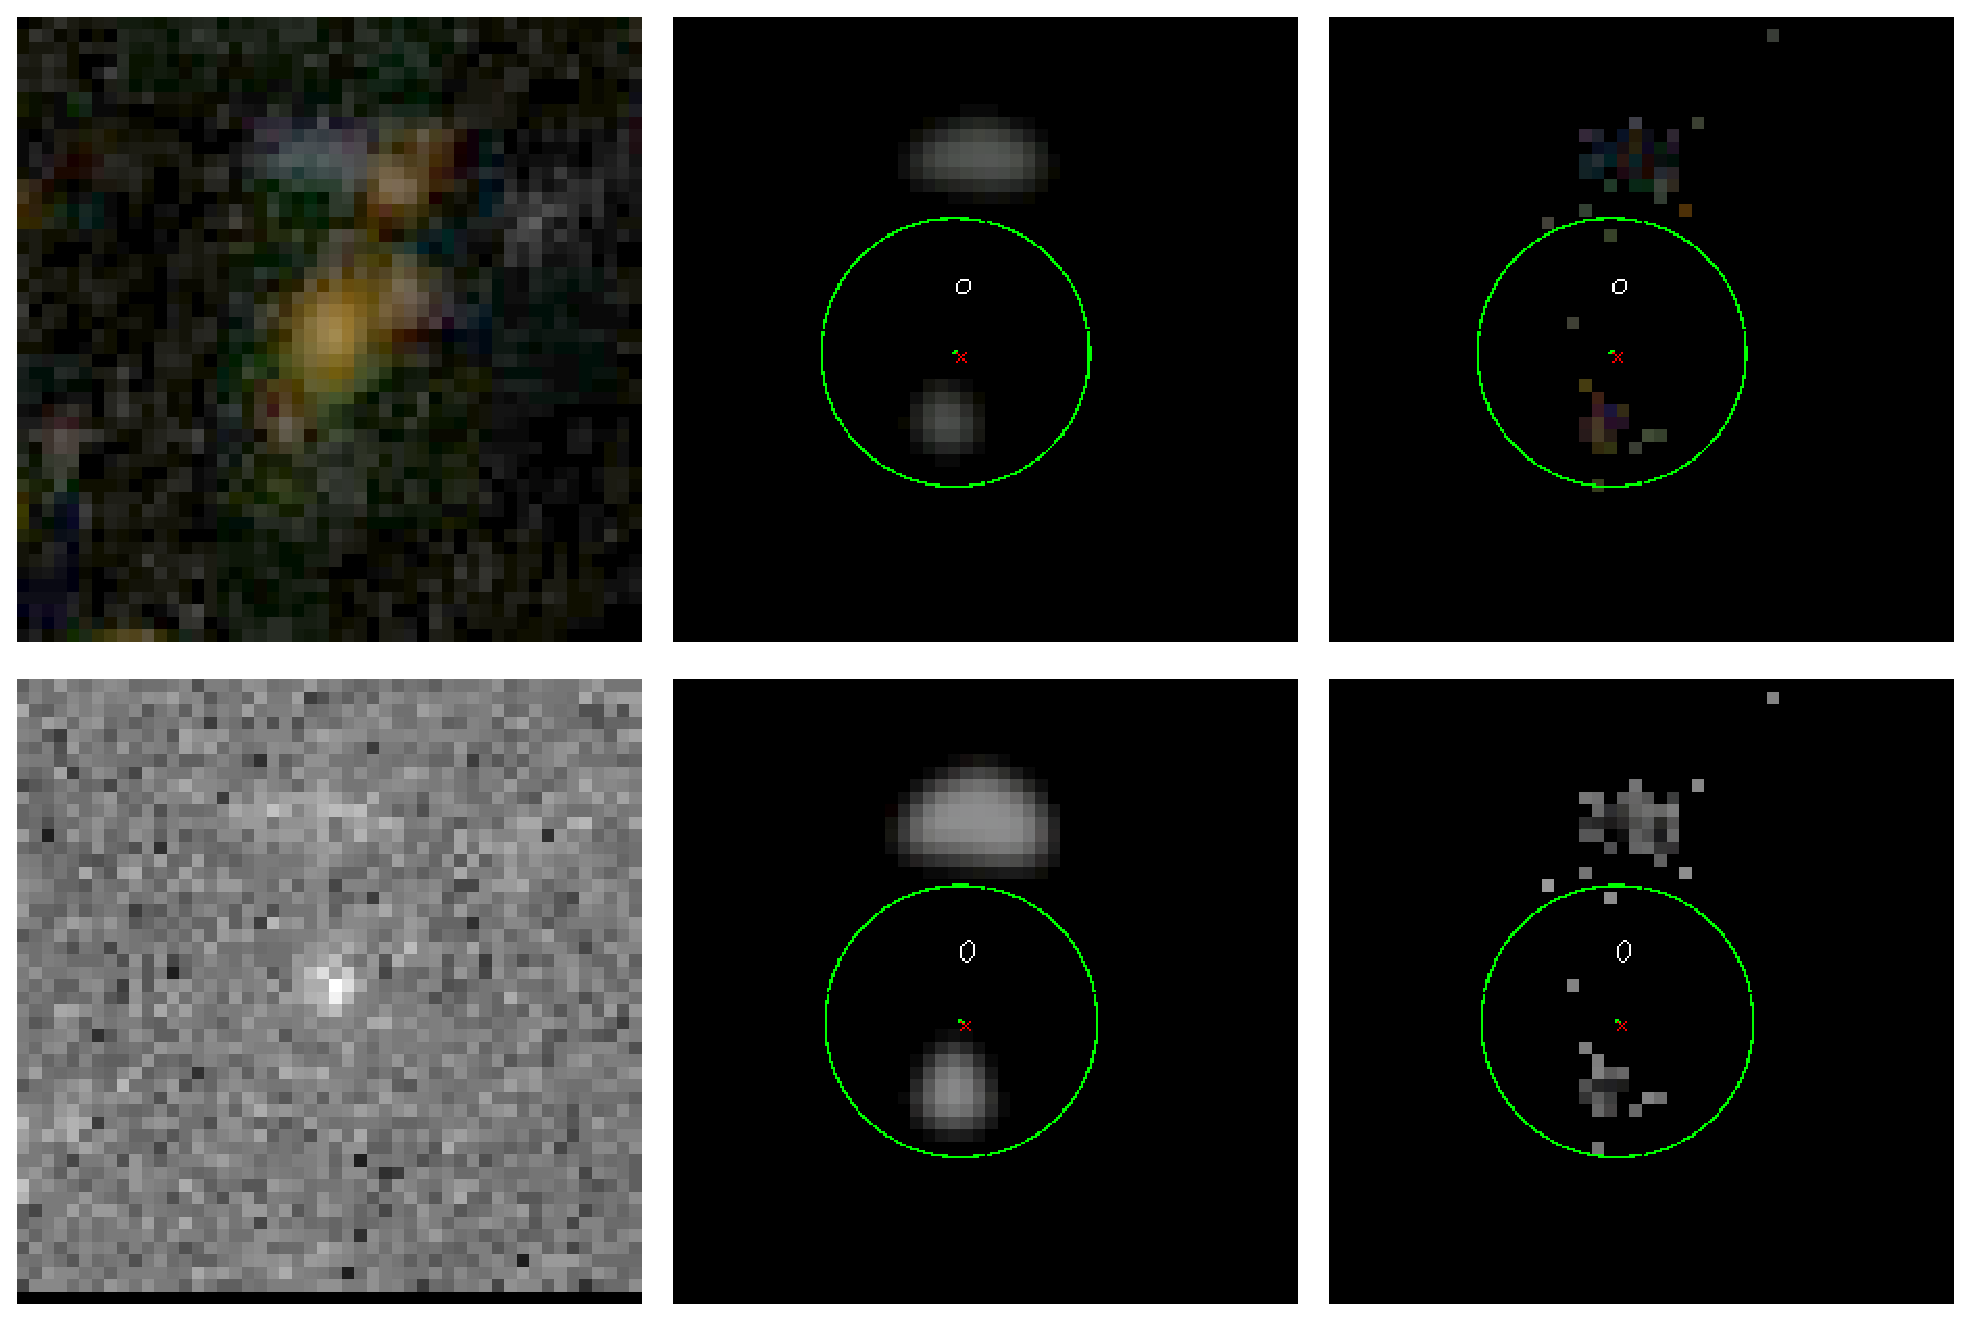
\includegraphics[width=\linewidth]{figs/17.eps}
	\caption{CSWA 17, see Figure~\ref{fig:cswa1} for caption.}
	\label{fig:cswa17}
\end{figure}
%%%%%%%%%%%%%%%%%%%%%%%%%%%%%%%%%%%%%%%%%%

CSWA~17 is a bright red elliptical galaxy with a short blue arc located just off
its major axis; some faint blue emission is just visible on the opposite side of
the red galaxy, in the right position for a counter image. This candidate has
been modeled using a single lens and a single source. Using a single component
lens model, with mass oriented similarly to the lens light, we can predict the
arc position and shape reasonably well, with a faint counter-image to the South
of the lens galaxy consistent with the faint emission there. 


% . . . . . . . . . . . . . . . . . . . . . . . . . . . . . . . . . . . .  .  

\subsubsection*{CSWA~18: SDSS\ J1134$+$2533}
\label{sec:results:indinotes:cswa18}

% {\bf CLASSIFICATION: X}

%%%%%%%%%%%%%%%%%%%%%%%%%%%%%%%%%%%%%%%%%%
\begin{figure}[!ht]
	\centering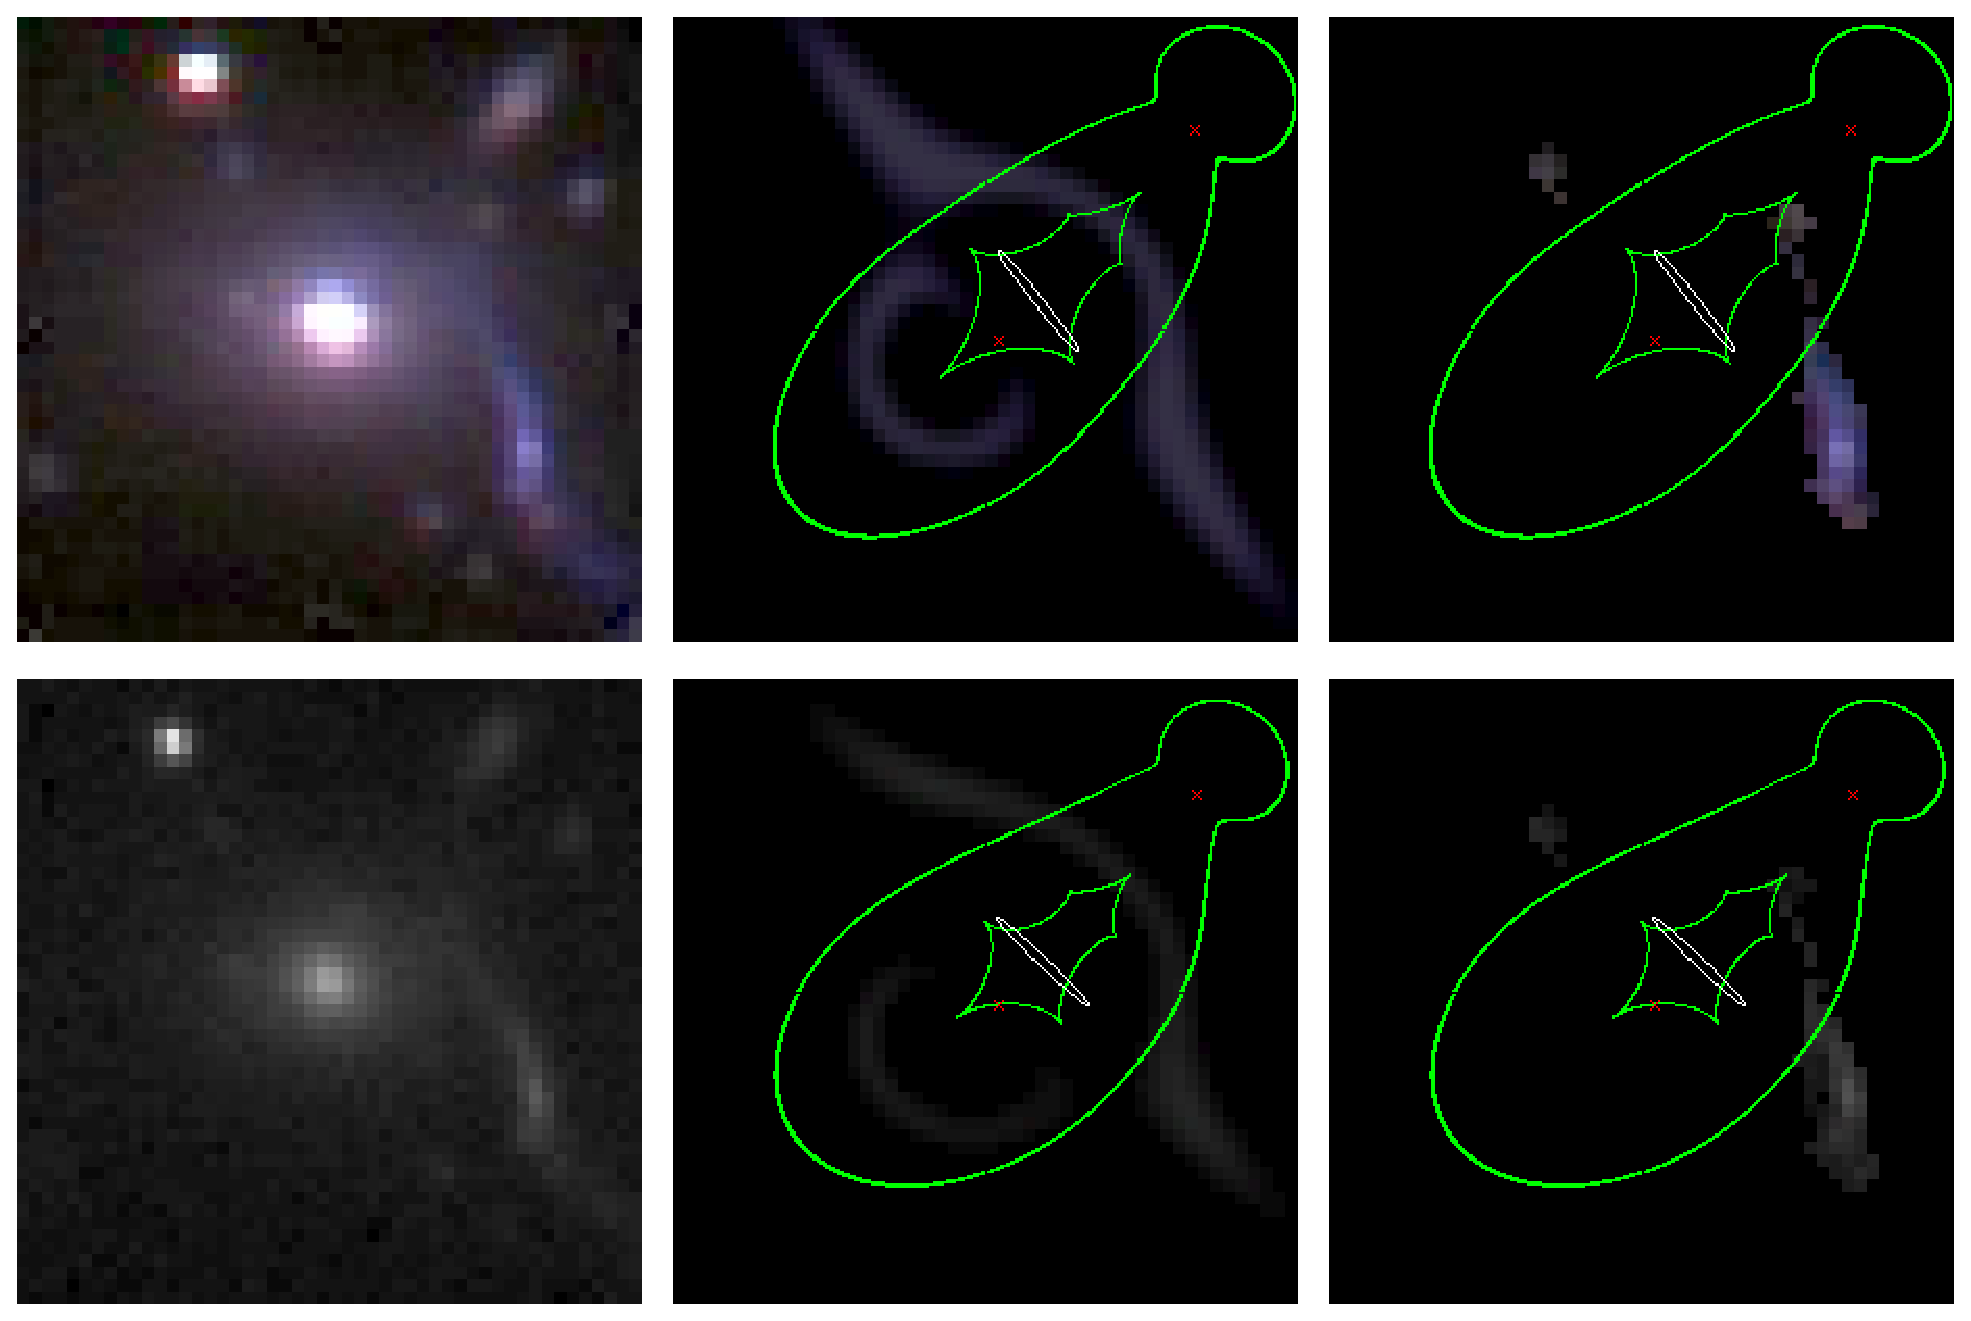
\includegraphics[width=\linewidth]{figs/18.eps}
	\caption{CSWA 18, see Figure~\ref{fig:cswa1} for caption.}
	\label{fig:cswa18}
\end{figure}
%%%%%%%%%%%%%%%%%%%%%%%%%%%%%%%%%%%%%%%%%%

CSWA~18 is the lowest redshift CASSOWARY lens candidate. The candidate lens
candidate is part of a linear structure aligned approximately East-West on the
sky. The proposed lensed feature is a blue arc spiraling in towards the central
LRG. We modelled this candidate using two lens components --  the main LRG and a
bright satellite to the North-West -- and a single source. The arc can be
predicted by this model, with the right position, shape and orientation,
provided the main lens mass distribution is highly elongated and the source has
a low axis ratio (like an edge-on disk). The lens elongation is, however,
aligned with the larger structure, adding plausibility to this model.  The
problem is that the model predicts counter arcs of comparable brightness that
are not observed: these counter-arcs fall in regions that were masked to remove
the lens galaxy light (so that the $\Omega$ value is misleadingly high), but
they are bright enough to be clearly visible in the original image. Finally, the
Einstein radius of the main lens component is some 11~arcsec, very high for such
a low redshift, non-cluster lens.

It is very likely that the arc in this image is not a lensed background
feature.  Instead, the arc might be a one-arm spiral created by a recent
interaction. The colors are consistent with the outer disk of the primary
galaxy, and the arc seems to be attached to this disk. A measurement of the 
redshift of the arc would completely resolve this issue. Until then, the
difficulty in modeling this system with a plausible mass distribution such that
no detectable counter-images are predicted suggests that this is not a typical
gravitational lens.


% . . . . . . . . . . . . . . . . . . . . . . . . . . . . . . . . . . . .  .  

\subsubsection*{CSWA~19: SDSS\ J0900$+$2234}
\label{sec:results:indinotes:cswa19}

% {\bf CLASSIFICATION: A}

%%%%%%%%%%%%%%%%%%%%%%%%%%%%%%%%%%%%%%%%%%
\begin{figure}[!ht]
	\centering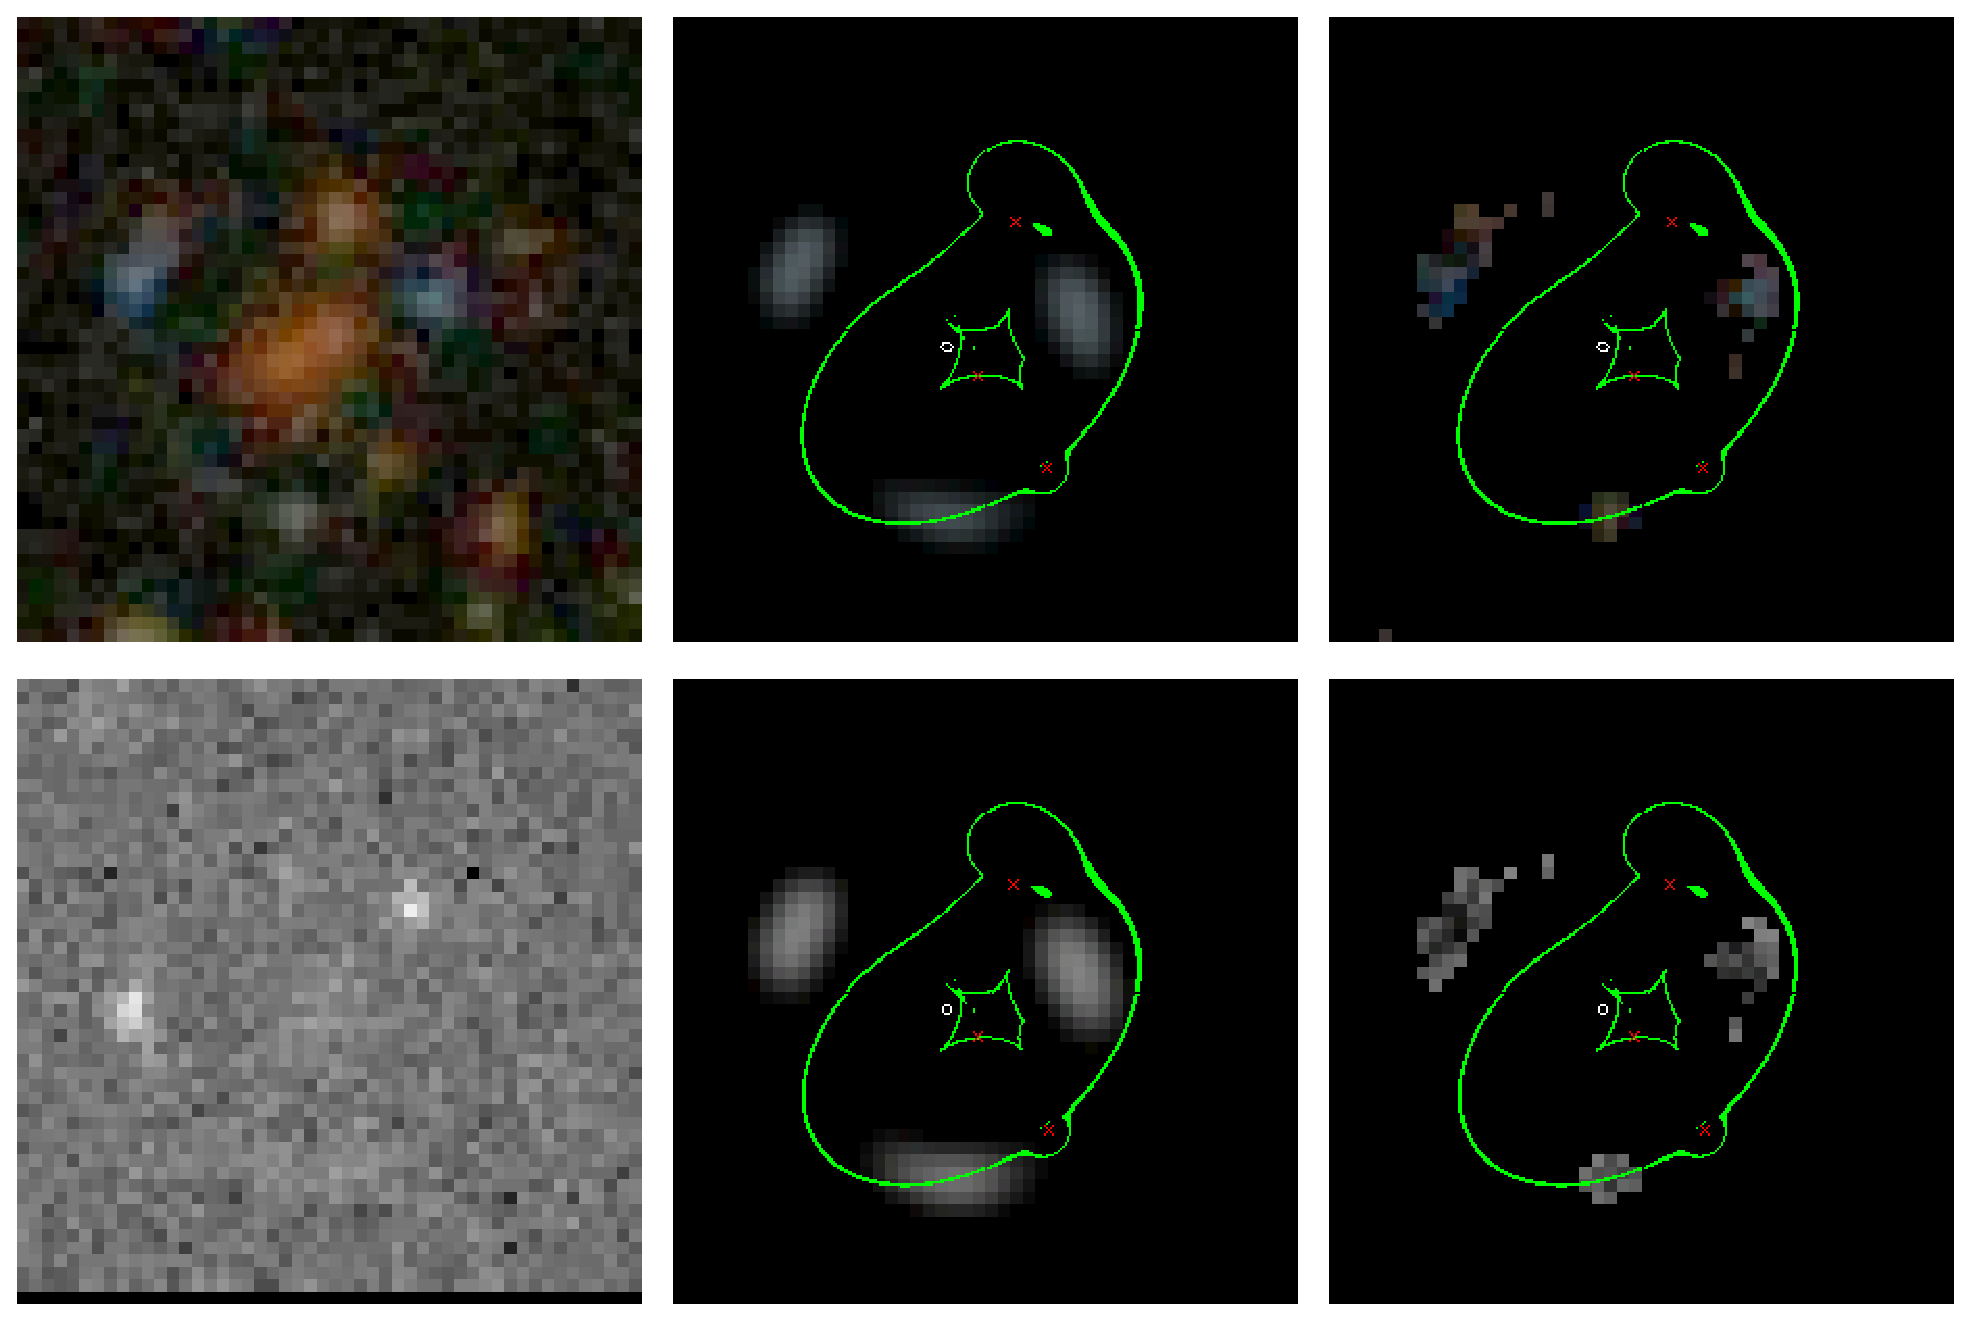
\includegraphics[width=\linewidth]{figs/19.eps}
	\caption{CSWA 19, see Figure~\ref{fig:cswa1} for caption.}
	\label{fig:cswa19}
\end{figure}
%%%%%%%%%%%%%%%%%%%%%%%%%%%%%%%%%%%%%%%%%%

This candidate was modelled as a simple single-lens system by \citet{Die++09}, 
who showed that the blue knots to the West and East of the bright central pair
of galaxies have the same redshift. Using a single elliptical mass component
centered on and aligned with this pair, we were able to approximately predict
the positions of the  two blue images, and predict a counter-arc to the South
coincident with third blue-ish image. We obtain a better fit when we include
small mass components associated with red satellite galaxies to the North and
South: the predicted images also have relative brightnesses that match the
observed ones. We note that our predicted image positions  are not accurate
enough to obtain an $\Omega$ better than 44\%, and that we can achieve  $\Omega
\simeq 75\%$ with a model that has three singly-imaged sources. However, the
lensing hypothesis has much greater simplicity, and therefore plausibility: with
further  tweaking we expect the lens model goodness of fit to improve.

The Einstein radius of the main lens component in our model is $6.4\pm0.1$~arcsec, 
in agreement with the rough estimate of $7\pm0.8$ arcsec from \citet{Die++09}. 
Despite the source lying close to a swallowtail caustic the predicted magnification is fairly low 
($\sim 4$).


% . . . . . . . . . . . . . . . . . . . . . . . . . . . . . . . . . . . .  .  

\subsubsection*{CSWA~20: SDSS\ J1441$+$1441}
\label{sec:results:indinotes:cswa20}

% {\bf CLASSIFICATION: A}

%%%%%%%%%%%%%%%%%%%%%%%%%%%%%%%%%%%%%%%%%%
\begin{figure}[!ht]
	\centering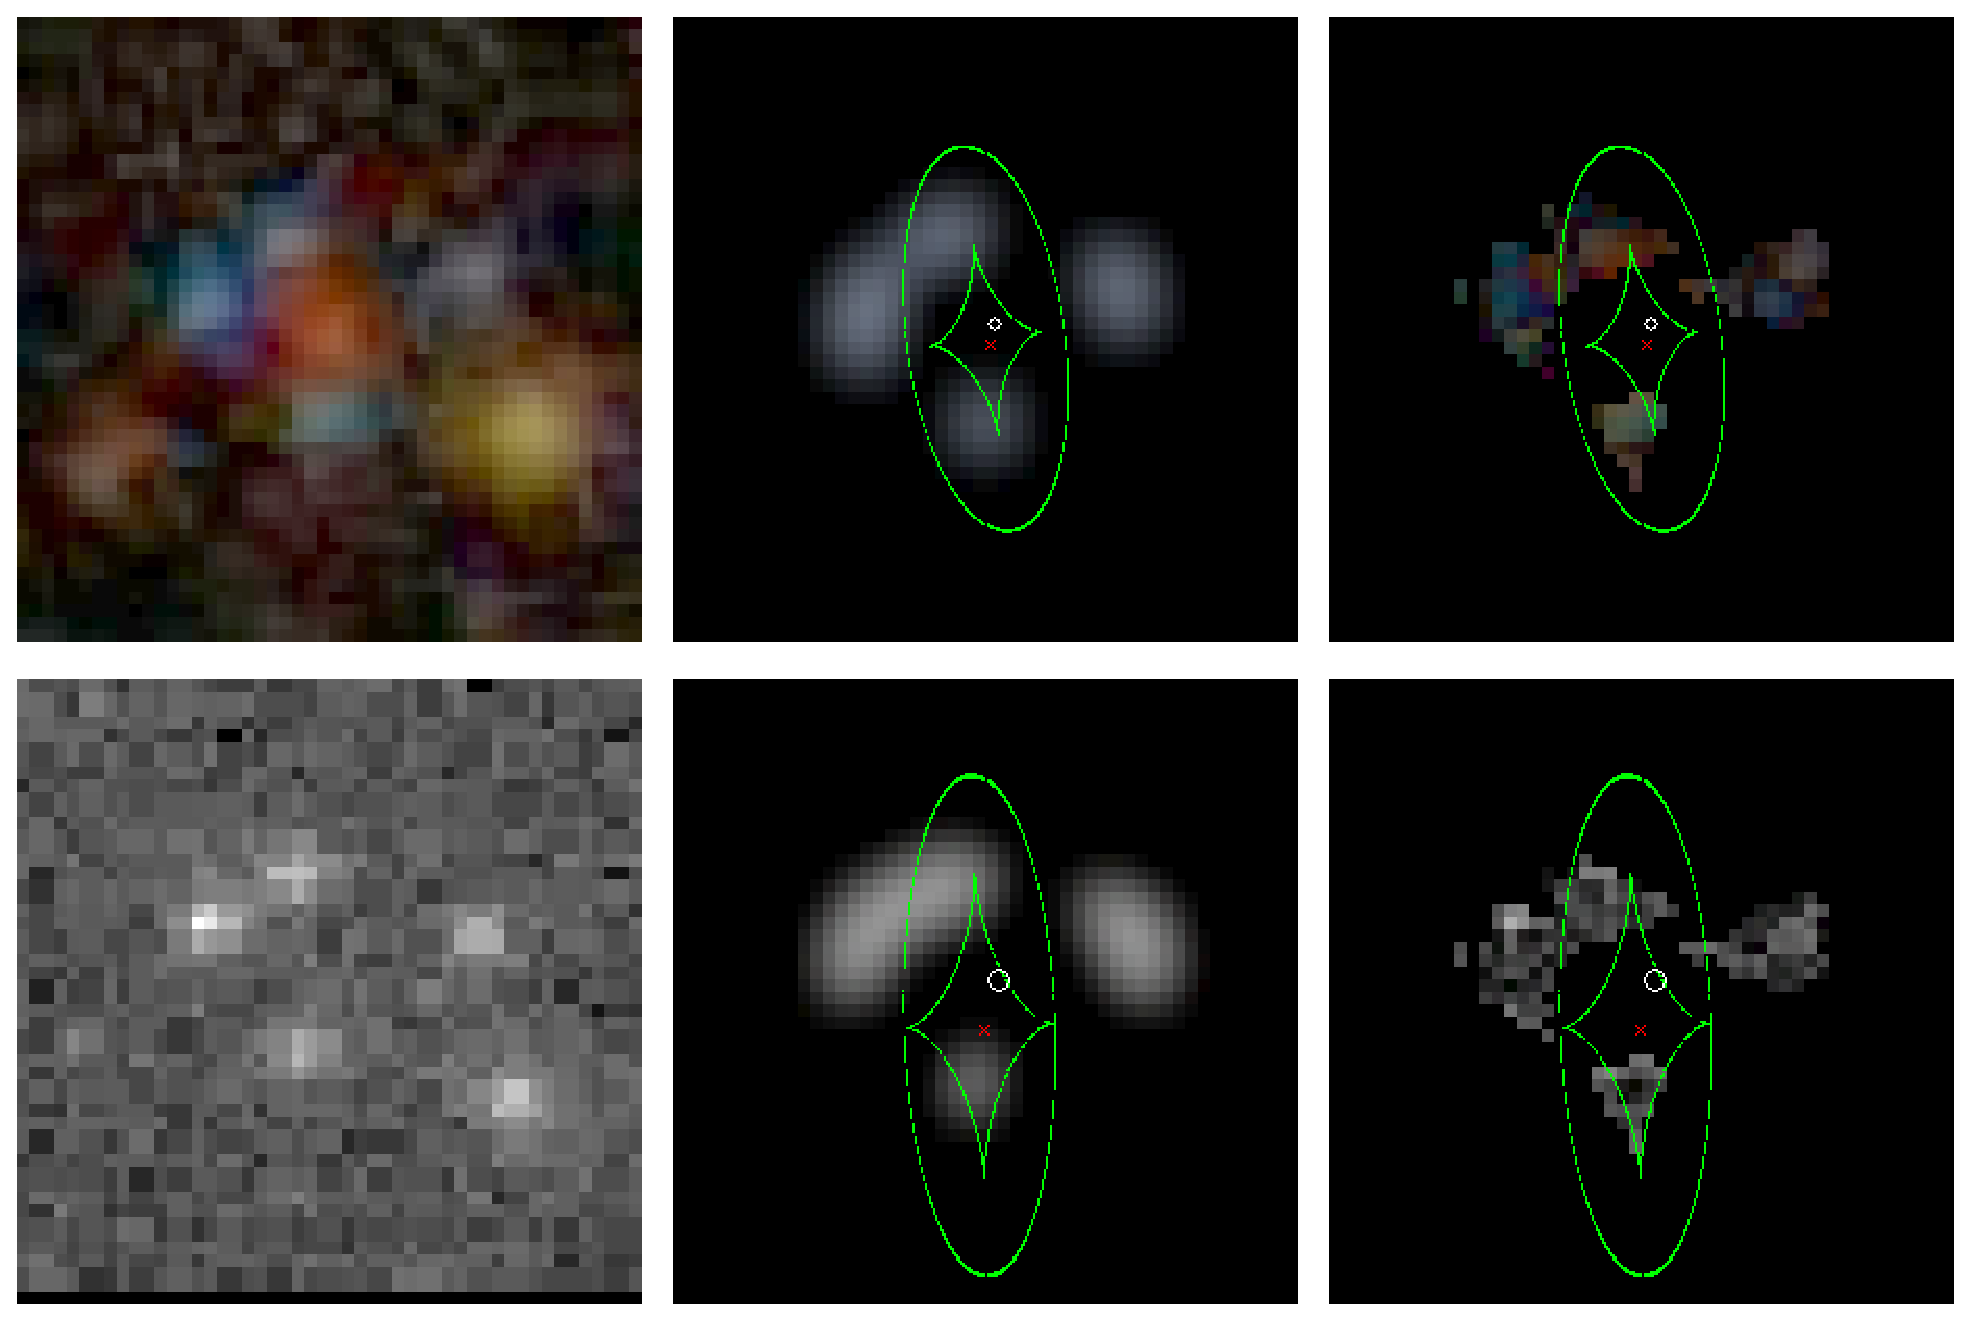
\includegraphics[width=\linewidth]{figs/20.eps}
	\caption{CSWA 20, see Figure~\ref{fig:cswa1} for caption.}
	\label{fig:cswa20}
\end{figure}
%%%%%%%%%%%%%%%%%%%%%%%%%%%%%%%%%%%%%%%%%%

This candidate is a relatively simple system, a red galaxy apparently lensing a
blue source into four images. A model consisting of a single SIE lens and a
single source is able to reproduce all four of the image positions accurately.

The Einstein radius of the main lens component is $3.1 \pm 0.1$~arcsec. Using
the redshifts of the source and lens galaxies presented by \citeauthor{Pet++10},
we determined the velocity dispersion parameter of the SIE model to be $458 \pm
7$ km/s, which is within one standard deviation of the stellar velocity
dispersion which \citet{Pet++10} present.

\citeauthor{Pet++10} determined the magnification of this lens to be $\sim 6$,
somewhat lower than that predicted by our model ($\sim 11$). 

%  -  -  -  -  -  -  -  -  -  -  -  -  -  -  -  -  -  -  -  -  -  -  -  -  -  

\subsection{Lens candidate classification}
\label{sec:results:class}

In the cases where a model's predictions gave a good visual fit to the data,
the $\Omega$ value was found to be around $80\%-90\%$. Some models gave  lower
values -- these correspond to mismatches in the detailed morphology of the
predicted arcs, and the presence of significant counter-image features. We use
these quantified residuals to inform a lens classification.

Based on our modeling, we assign each system a subjective classification, 
similar to those assigned by \eg \citet{Bol++08} and \citet{Mar++09}. In this
scheme, we use
\begin{description}
  \item{``A'' to mean ``definitely a lens''} -- a plausible model fits all
  identified features and does not predict any detectable but unobserved ones.
  \item{``B'' to mean ``probably a lens''} -- a plausible model  fits most of
  the identified lensed features, but perhaps not very well in some cases; some
  models may do better but predict counter-images that may be detectable but
  are  not observed. Likewise, the model may predict the required multiple
  images very well, but itself be implausible (perhaps containing additional
  unseen mass components, large centroid offsets,  or high ellipticity.
  \item{``C'' to mean ``possibly a lens''} -- the features are reminiscent of
  strong lensing (long, curved arcs or systems of potentially matching conjugate
  images), but no model can fit them sufficiently well as to provide a
  convincing multiple imaging scenario. This class includes short, straight,
  single arcs with no visible  counter-images, pairs of images with almost the
  same color but odd positions and so on. 
  \item{``X'' to mean ``definitely not a lens''} -- no model can be found which
  predicts the observed features using multiple imaging. 
\end{description}
Typically,  good additional data is required to either upgrade a class B
candidate to a grade A lens, or to downgrade a C-grade candidate to one in the X
class. The CASSOWARY  sample is pre-selected to contain candidates that are
either grade A, B or C, with a strong preference for A and B grades; we leave
the complementary investigation of poorer quality  grade C candidates and known
(false positive) non-lenses to further work. Our aim here is to show that when
the features are due to lensing, we can fit them -- and provide a model-based
classification (A, B, or C) for all systems in the sample.


%  -  -  -  -  -  -  -  -  -  -  -  -  -  -  -  -  -  -  -  -  -  -  -  -  -  

\subsection{JPEG and FITS Results}
\label{sec:results:JPEGvsFITS}

\NEW{As mentioned in Section \ref{sec:chiSq}, the uncertainties of the JPEG
and FITS models have been computed independently, in order that they might be
compared against each other.  Due to JPEG compression, the errors of the JPEG
uncertainties tend to be considerably larger than the errors of FITS
uncertainties. From the similarity of the inferred parameters in
Table~\ref{tab:all}, we conclude that \theapplet may be used to successfully
model systems using JPEG images, although the resulting parameter
uncertainties will be somewhat less robust.}

We find that the two goodness of fit statistics
we use are approximately linearly related to each other,

$\rchisq_\text{JPEG} = \gamma
\chi^2_\text{FITS}$. A regression analysis of the 20 analysed systems 
gives $\gamma = 0.175 \pm
0.70$. 

Using linear
regression, we determined that $\rchisq_\text{JPEG} \approx 1.34
\chisq_\text{FITS} + 106.85$. 

Thus, when we chose to let $\delta_\text{FITS} = 1$
and $\delta_\text{JPEG} = 1.34$.

\ACHTUNG{PSN}{These scalings are inconsistent, which is correct? More
seriously, we now have crazy small uncertainties on the parameters, I guess
coming from the FITS analysis. I don't believe them! They are obviously too
small, no? This could be due to only varying one prameter at a time (the
multi-variate likelihood function could be strongly covariant), or there could
be a bug. Either way, we cannot publish such values! Fortunately only the
table has changed, th e individual notes text is still the same -- I'll
revisit the referee report and see what we need to do...}

%  -  -  -  -  -  -  -  -  -  -  -  -  -  -  -  -  -  -  -  -  -  -  -  -  -  

\subsection{The Properties of the Sample}
\label{sec:results:summary}

We give the optimized model parameters, and our lens classifications, for the
CASSOWARY systems in  Table~\ref{tab:models}.

%%%%%%%%%%%%%%%%%%%%%%%%%%%%
\begin{table*}
\begin{center}
\caption{Parameters for \theapplet lens models illustrated in
Section~\ref{sec:results.indi}.}
\scriptsize
\renewcommand{\arraystretch}{1.5}
\begin{tabular*}{\linewidth}{@{\extracolsep{\fill}}c c ccccc c ccccc c ccc}
%%%%%%%
\hline\hline
%          & \multicolumn{5}{c}{Lens Properties}                                      & \multicolumn{5}{c}{Source Properties}                                     &             &       &            \\
%     ID   & $\xd (")$     & $\yd (")$    & $\Rein(")$ & $\qd\;\;\;\;$  & $\phid$(rad)
%          & $\xs(")$     & $\ys(")$     & $\Reff(")$  & $\epsilon\;\;\;\;$ & $\phis$(rad)    & $\chi^2$  & Class & $\mu$      \\ \hline\hline \smallskip
\multicolumn{1}{c}{~}                 & \multicolumn{1}{c}{~~~} &
\multicolumn{5}{c}{Lens Properties}   & \multicolumn{1}{c}{~~~} &
\multicolumn{5}{c}{Source Properties} & \multicolumn{1}{c}{~~~} &
\multicolumn{3}{c}{~} \\
%%%%%%%
\multicolumn{1}{c}{ID} &
%
\multicolumn{1}{c}{} &
%
\multicolumn{1}{c}{$\xd (")$} &
\multicolumn{1}{c}{$\yd (")$} &
\multicolumn{1}{c}{$\Rein(")$} &
\multicolumn{1}{c}{$\qd$} &
\multicolumn{1}{c}{$\phid$(rad)} &
%
\multicolumn{1}{c}{} &
%
\multicolumn{1}{c}{$\xs(")$} &
\multicolumn{1}{c}{$\ys(")$} &
\multicolumn{1}{c}{$\Reff(")$} &
\multicolumn{1}{c}{$\qs$} &
\multicolumn{1}{c}{$\phis$(rad)} &
%
\multicolumn{1}{c}{} &
%
\multicolumn{1}{c}{$\chi^2$} &
\multicolumn{1}{c}{Class} &
\multicolumn{1}{c}{$\mu$} \smallskip \\
%
%%%%%%%
\cline{1-1}\cline{3-7}\cline{9-13}\cline{15-17}
%%%%%%%
      \multirow{1}{*}{1$_{\rm F}$}
           & & $0.0169\pm0.0003$  & $-0.2958\pm0.0004$  & $5.7989\pm0.0002$  & $0.7401\pm0.0004$  & $0.8023\pm0.0001$   & & $0.2038\pm0.0002$  & $0.3587\pm0.0001$  & $0.3841\pm0.0001$  & $0.5871\pm0.0002$  & $0.3164\pm0.0002$& & 931 & A & $ 20.9 \pm X$  \\\cline{1-1}\cline{3-7}\cline{9-13}\cline{15-17}
      \multirow{1}{*}{1$_{\rm J}$}
           & & $0.1501\pm0.0001$  & $-0.2783\pm0.0002$  & $5.9698\pm0.0003$  & $0.7932\pm0.0001$  & $0.7698\pm0.0002$   & & $0.2079\pm0.0001$  & $0.2852\pm0.0001$  & $0.3500\pm0.0001$  & $0.7197\pm0.0003$  & $0.2799\pm0.0004$& & 986 & A & $ 23.0 \pm X$  \\\cline{1-1}\cline{3-7}\cline{9-13}\cline{15-17}
% - - - - - - - - - - - - - - - - - - - - - - - - - - - - - - - - - - - - - - - - - - - - - - - - - - - - - - - - - - - - - - - - - - - - - - - - - - - - - - - - - - - - - - - - - - - - - - - - - - - - - - - - - - - - - - - - - - - - - - - - - - - - - - - - - - - -
      \multirow{2}{*}{2$_{\rm F}$}
           & & $-8.0506\pm0.0015$  & $-2.0937\pm0.0025$  & $4.2555\pm0.0007$  & $0.2310\pm0.0002$  & $2.1507\pm0.0003$   & & $-1.9886\pm0.0005$  & $-0.0329\pm0.0011$  & $0.6010\pm0.0003$  & $1.0000\pm0.0011$  & $0.9820\pm\infty$& & 2132 & A & $ 14.2 \pm X$  \\
					 & & $0.2207\pm0.0015$  & $-0.0742\pm0.0011$  & $6.4141\pm0.0007$  & $0.7568\pm0.0003$  & $2.6602\pm0.0011$   & & $-1.9035\pm0.0009$  & $-1.8186\pm0.0013$  & $2.0249\pm0.0006$  & $1.0000\pm0.0003$  & $0.3864\pm\infty$& &      &   &            \\\cline{1-1}\cline{3-7}\cline{9-13}\cline{15-17}
      \multirow{2}{*}{2$_{\rm J}$}
           & & $-8.0125\pm0.0005$  & $-2.3427\pm0.0005$  & $6.0308\pm0.0002$  & $0.9994\pm0.0002$  & $0.9592\pm\infty$   & & $-4.9580\pm0.0003$  & $1.4778\pm0.0002$  & $0.4361\pm0.0002$  & $0.9997\pm0.0004$  & $0.5651\pm\infty$& & 36408 & A & $ 13.3 \pm X$  \\
					 & & $0.9757\pm0.0003$  & $-1.1786\pm0.0005$  & $6.0283\pm0.0002$  & $0.4564\pm0.0001$  & $0.0072\pm0.0002$   & & $-1.3002\pm0.0029$  & $-1.9740\pm0.0023$  & $1.6940\pm0.0006$  & $1.0000\pm0.0006$  & $0.9504\pm\infty$& &      &   &            \\\cline{1-1}\cline{3-7}\cline{9-13}\cline{15-17}
% - - - - - - - - - - - - - - - - - - - - - - - - - - - - - - - - - - - - - - - - - - - - - - - - - - - - - - - - - - - - - - - - - - - - - - - - - - - - - - - - - - - - - - - - - - - - - - - - - - - - - - - - - - - - - - - - - - - - - - - - - - - - - - - - - - - -
      \multirow{1}{*}{3$_{\rm F}$}
           & & $1.9394\pm0.0001$  & $-1.6096\pm0.0001$  & $3.3300\pm0.0001$  & $0.3341\pm0.0001$  & $2.5473\pm0.0002$   & & $0.1051\pm0.0003$  & $0.1780\pm0.0001$  & $0.7824\pm0.0001$  & $0.3219\pm0.0001$  & $3.1280\pm0.0001$& & 1543 & A & $ 4.2 \pm X$  \\\cline{1-1}\cline{3-7}\cline{9-13}\cline{15-17}
      \multirow{1}{*}{3$_{\rm J}$}
           & & $1.5830\pm0.0002$  & $-1.4170\pm0.0004$  & $3.2320\pm0.0002$  & $0.3157\pm0.0001$  & $2.4280\pm0.0001$   & & $0.0829\pm0.0006$  & $0.0394\pm0.0002$  & $0.7387\pm0.0001$  & $0.5357\pm0.0001$  & $3.0825\pm0.0003$& & 1535 & A & $ 5.8 \pm X$  \\\cline{1-1}\cline{3-7}\cline{9-13}\cline{15-17}
% - - - - - - - - - - - - - - - - - - - - - - - - - - - - - - - - - - - - - - - - - - - - - - - - - - - - - - - - - - - - - - - - - - - - - - - - - - - - - - - - - - - - - - - - - - - - - - - - - - - - - - - - - - - - - - - - - - - - - - - - - - - - - - - - - - - -
      \multirow{3}{*}{4$_{\rm F}$}
			           & & $8.2086\pm\infty$  & $-0.5885\pm0.0025$  & $3.7335\pm0.0018$  & $0.2456\pm0.0003$  & $0.0811\pm0.0003$   & & $2.3537\pm0.0015$  & $-1.7409\pm0.0011$  & $0.7454\pm0.0003$  & $1.0000\pm0.0007$  & $1.8885\pm\infty$& & 479 & B & $ 4.2 \pm X$  \\
								 & & $1.0914\pm\infty$  & $-1.8527\pm0.0051$  & $2.9336\pm0.0016$  & $0.1651\pm0.0004$  & $0.7036\pm0.0009$   & &               &               &              &               &            & &      &   &            \\
								 & & $9.9146\pm\infty$  & $-7.2593\pm0.0045$  & $3.1536\pm0.0011$  & $0.9615\pm0.0018$  & $2.8973\pm\infty$   & &               &               &              &               &            & &      &   &            \\\cline{1-1}\cline{3-7}\cline{9-13}\cline{15-17}
      \multirow{3}{*}{4$_{\rm J}$}
           & & $8.3751\pm0.0059$  & $-0.4255\pm\infty$  & $3.6577\pm0.0008$  & $0.1953\pm0.0002$  & $0.0873\pm0.0003$   & & $2.0995\pm0.0011$  & $-1.8531\pm0.0011$  & $0.8645\pm0.0003$  & $1.0000\pm0.0003$  & $2.0737\pm\infty$& & 1155 & B & $ 4.1 \pm X$  \\
					 & & $1.2606\pm0.0012$  & $-1.9388\pm0.0052$  & $3.0402\pm0.0014$  & $0.1787\pm0.0003$  & $0.6396\pm0.0008$   & &               &               &              &               &            & &      &   &            \\
					 & & $10.0072\pm\infty$  & $-7.4411\pm0.0038$  & $3.4522\pm0.0006$  & $0.9748\pm0.0012$  & $2.7109\pm\infty$   & &               &               &              &               &            & &      &   &            \\\cline{1-1}\cline{3-7}\cline{9-13}\cline{15-17}
% - - - - - - - - - - - - - - - - - - - - - - - - - - - - - - - - - - - - - - - - - - - - - - - - - - - - - - - - - - - - - - - - - - - - - - - - - - - - - - - - - - - - - - - - - - - - - - - - - - - - - - - - - - - - - - - - - - - - - - - - - - - - - - - - - - - -
      \multirow{2}{*}{5$_{\rm F}$}
           & & $2.7521\pm0.0002$  & $0.7986\pm0.0002$  & $1.6331\pm0.0001$  & $1.0000\pm0.0002$  & $2.1262\pm\infty$   & & $-0.8848\pm0.0001$  & $-0.2669\pm0.0001$  & $0.1683\pm0.0001$  & $1.0000\pm0.0001$  & $2.4149\pm\infty$& & 1075 & A & $ 12.5 \pm X$  \\
					 & & $-2.9701\pm0.0001$  & $-0.3090\pm0.0001$  & $2.2273\pm0.0001$  & $1.0000\pm0.0001$  & $2.2294\pm\infty$   & &               &               &              &               &            & &      &   &            \\\cline{1-1}\cline{3-7}\cline{9-13}\cline{15-17}
      \multirow{2}{*}{5$_{\rm J}$}
           & & $3.0801\pm0.0006$  & $0.5010\pm0.0003$  & $1.7504\pm0.0001$  & $1.0000\pm0.0002$  & $1.7308\pm\infty$   & & $-0.6741\pm0.0001$  & $-0.5202\pm0.0001$  & $0.2710\pm0.0001$  & $1.0000\pm0.0003$  & $2.8797\pm\infty$& & 1797 & A & $ 9.0 \pm X$  \\
					 & & $-3.0522\pm0.0002$  & $-0.4250\pm0.0001$  & $2.1884\pm0.0002$  & $1.0000\pm0.0001$  & $2.1291\pm\infty$   & &               &               &              &               &            & &      &   &            \\\cline{1-1}\cline{3-7}\cline{9-13}\cline{15-17}
% - - - - - - - - - - - - - - - - - - - - - - - - - - - - - - - - - - - - - - - - - - - - - - - - - - - - - - - - - - - - - - - - - - - - - - - - - - - - - - - - - - - - - - - - - - - - - - - - - - - - - - - - - - - - - - - - - - - - - - - - - - - - - - - - - - - -
      \multirow{1}{*}{6$_{\rm F}$}
           & & $-0.4670\pm0.0005$  & $-0.4550\pm0.0005$  & $3.8912\pm0.0006$  & $0.5697\pm0.0004$  & $0.2607\pm0.0002$   & & $0.7791\pm0.0003$  & $0.4362\pm0.0005$  & $0.3499\pm0.0001$  & $0.9816\pm0.0005$  & $2.6588\pm\infty$& & 922 & A & $ 5.8 \pm X$  \\\cline{1-1}\cline{3-7}\cline{9-13}\cline{15-17}
      \multirow{1}{*}{6$_{\rm J}$}
           & & $-0.0057\pm0.0005$  & $-0.4325\pm0.0004$  & $3.7760\pm0.0003$  & $0.6094\pm0.0002$  & $0.2377\pm0.0002$   & & $0.8456\pm0.0002$  & $0.1351\pm0.0001$  & $0.2926\pm0.0001$  & $0.9842\pm0.0003$  & $2.8151\pm\infty$& & 1140 & A & $ 9.5 \pm X$  \\\cline{1-1}\cline{3-7}\cline{9-13}\cline{15-17}
% - - - - - - - - - - - - - - - - - - - - - - - - - - - - - - - - - - - - - - - - - - - - - - - - - - - - - - - - - - - - - - - - - - - - - - - - - - - - - - - - - - - - - - - - - - - - - - - - - - - - - - - - - - - - - - - - - - - - - - - - - - - - - - - - - - - -
      \multirow{1}{*}{7a$_{\rm F}$}
           & & $-0.6025\pm0.0005$  & $-0.0228\pm0.0002$  & $2.4870\pm0.0002$  & $0.1794\pm0.0001$  & $2.6766\pm0.0001$   & & $-2.0853\pm0.0001$  & $0.9694\pm0.0001$  & $0.1545\pm0.0001$  & $0.7911\pm0.0004$  & $2.8554\pm0.0010$& & 417 & B & $ 6.4 \pm X$  \\\cline{1-1}\cline{3-7}\cline{9-13}\cline{15-17}
      \multirow{1}{*}{7a$_{\rm J}$}
           & & $-0.3032\pm0.0003$  & $-0.1576\pm0.0002$  & $2.6177\pm0.0002$  & $0.1888\pm0.0001$  & $2.7032\pm0.0002$   & & $-1.7920\pm0.0002$  & $0.7744\pm0.0001$  & $0.2925\pm0.0001$  & $0.4878\pm0.0003$  & $3.0998\pm0.0005$& & 597 & B & $ 6.4 \pm X$  \\\cline{1-1}\cline{3-7}\cline{9-13}\cline{15-17}
% - - - - - - - - - - - - - - - - - - - - - - - - - - - - - - - - - - - - - - - - - - - - - - - - - - - - - - - - - - - - - - - - - - - - - - - - - - - - - - - - - - - - - - - - - - - - - - - - - - - - - - - - - - - - - - - - - - - - - - - - - - - - - - - - - - - -
	\multirow{2}{*}{7b$_{\rm F}$}
           & & $0.3338\pm0.0005$  & $-0.4025\pm0.0002$  & $2.7504\pm0.0001$  & $0.6659\pm0.0001$  & $2.8370\pm0.0003$   & & $-1.0126\pm0.0002$  & $1.0919\pm0.0005$  & $0.1071\pm0.0001$  & $0.9924\pm0.0018$  & $2.9020\pm\infty$& & 367 & B & $ 4.0 \pm X$  \\
					 & &               &               &              &               &               & & $-1.3525\pm0.0002$  & $-0.0321\pm0.0002$  & $0.1659\pm0.0001$  & $0.6490\pm0.0007$  & $0.1150\pm0.0006$& &      &   &            \\\cline{1-1}\cline{3-7}\cline{9-13}\cline{15-17}
	\multirow{2}{*}{7b$_{\rm J}$}
           & & $0.4957\pm0.0002$  & $-0.5641\pm0.0002$  & $2.7608\pm0.0004$  & $0.7092\pm0.0001$  & $2.7348\pm0.0003$   & & $-0.7565\pm0.0009$  & $0.9445\pm0.0005$  & $0.1672\pm0.0002$  & $0.8216\pm0.0011$  & $2.9595\pm\infty$& & 518 & B & $ 3.7 \pm X$  \\
					 & &               &               &              &               &               & & $-1.2015\pm0.0002$  & $-0.1493\pm0.0002$  & $0.3554\pm0.0002$  & $0.5043\pm0.0002$  & $2.9943\pm0.0003$& &      &   &            \\\cline{1-1}\cline{3-7}\cline{9-13}\cline{15-17}
% - - - - - - - - - - - - - - - - - - - - - - - - - - - - - - - - - - - - - - - - - - - - - - - - - - - - - - - - - - - - - - - - - - - - - - - - - - - - - - - - - - - - - - - - - - - - - - - - - - - - - - - - - - - - - - - - - - - - - - - - - - - - - - - - - - - -
% OLD PSN MODEL:
%       \multirow{2}{*}{8}
%            & & $ 4\pm2$      & $-3\pm1$      & $1.6\pm0.2$  & $0.7\pm0.1$   & $1.2\pm0.4$   & & $-1.2\pm0.1$ & $-1.3\pm0.1$ & $0.8\pm0.1$   & $1.0\pm0.2$   & 0           & & 47\% & A & $14 \pm 7$    \\
%            & & $ 0.3\pm0.1$  & $-0.4\pm0.1$  & $6.3\pm0.1$  & $0.5\pm0.1$   & $2.6\pm0.1$   & &              &              &               &               &             & &      &   &            \\
%            & & $-0.8\pm0.2$  & $-6.6\pm0.3$  & $3.6\pm0.1$  & $0.7\pm0.1$   & $0.3\pm0.3$   & &              &              &               &               &             & &      &   &            \\ \cline{1-1}\cline{3-7}\cline{9-13}\cline{15-17}
% - - - - - - - - - - - - - - - - - - - - - - - - - - - - - - - - - - - - - - - - - - - - - - - - - - - - - - - - - - - - - - - - - - - - - - - - - - - - - - - - - - - - - - - - - - - - - - - - - - - - - - - - - - - - - - - - - - - - - - - - - - - - - - - - - - - -
      \multirow{1}{*}{8$_{\rm F}$}
           & & $0.9384\pm0.0067$  & $-0.1077\pm0.0046$  & $7.8527\pm0.0012$  & $0.5007\pm0.0008$  & $2.8410\pm0.0016$   & & $-3.2155\pm0.0033$  & $1.8441\pm0.0046$  & $0.4260\pm0.0004$  & $0.9882\pm0.0015$  & $1.6407\pm\infty$& & 368 & A & $ 5.9 \pm X$  \\\cline{1-1}\cline{3-7}\cline{9-13}\cline{15-17}
      \multirow{1}{*}{8$_{\rm J}$}
           & & $0.6438\pm0.0004$  & $-0.0912\pm0.0006$  & $7.8033\pm0.0003$  & $0.4324\pm0.0001$  & $2.8342\pm0.0002$   & & $-3.4690\pm0.0004$  & $1.7599\pm0.0002$  & $0.2748\pm0.0001$  & $0.9906\pm0.0003$  & $1.4383\pm0.0045$& & 1124 & A & $ 6.4 \pm X$  \\\cline{1-1}\cline{3-7}\cline{9-13}\cline{15-17}
% - - - - - - - - - - - - - - - - - - - - - - - - - - - - - - - - - - - - - - - - - - - - - - - - - - - - - - - - - - - - - - - - - - - - - - - - - - - - - - - - - - - - - - - - - - - - - - - - - - - - - - - - - - - - - - - - - - - - - - - - - - - - - - - - - - - -
      \multirow{4}{*}{9$_{\rm F}$}
           & & $4.1022\pm\infty$  & $1.8575\pm\infty$  & $2.2421\pm0.0035$  & $0.9288\pm0.0041$  & $0.6904\pm\infty$   & & $-0.4267\pm0.0028$  & $3.7810\pm0.0053$  & $0.4968\pm0.0008$  & $0.9811\pm0.0029$  & $1.4690\pm\infty$& & 327 & A & $ 6.0 \pm X$  \\
					 & & $-0.5513\pm0.0093$  & $0.8088\pm\infty$  & $2.4443\pm0.0032$  & $0.9641\pm\infty$  & $0.9707\pm\infty$   & &               &               &              &               &            & &      &   &            \\
					 & & $0.8718\pm\infty$  & $-1.0032\pm\infty$  & $2.9535\pm0.0030$  & $1.0000\pm0.0028$  & $1.3654\pm\infty$   & &               &               &              &               &            & &      &   &            \\
					 & & $-2.6316\pm\infty$  & $4.3168\pm\infty$  & $1.1984\pm0.0036$  & $1.0000\pm0.0077$  & $1.7704\pm\infty$   & &               &               &              &               &            & &      &   &            \\\cline{1-1}\cline{3-7}\cline{9-13}\cline{15-17}
      \multirow{4}{*}{9$_{\rm J}$}
           & & $3.9018\pm0.0028$  & $2.1214\pm\infty$  & $2.2290\pm0.0010$  & $0.9542\pm0.0010$  & $0.8754\pm\infty$   & & $-0.4526\pm0.0008$  & $3.7158\pm0.0014$  & $0.4098\pm0.0003$  & $1.0000\pm0.0004$  & $1.3576\pm\infty$& & 337 & A & $ 6.3 \pm X$  \\
					 & & $-0.6751\pm0.0044$  & $0.8817\pm0.0050$  & $2.3430\pm0.0010$  & $0.9205\pm0.0014$  & $1.1304\pm\infty$   & &               &               &              &               &            & &      &   &            \\
					 & & $0.7991\pm0.0036$  & $-0.9545\pm0.0024$  & $2.9005\pm0.0010$  & $1.0000\pm0.0015$  & $1.4358\pm\infty$   & &               &               &              &               &            & &      &   &            \\
					 & & $-2.8187\pm\infty$  & $4.4102\pm\infty$  & $1.2373\pm0.0006$  & $0.9724\pm0.0023$  & $1.7748\pm\infty$   & &               &               &              &               &            & &      &   &            \\\cline{1-1}\cline{3-7}\cline{9-13}\cline{15-17}
% - - - - - - - - - - - - - - - - - - - - - - - - - - - - - - - - - - - - - - - - - - - - - - - - - - - - - - - - - - - - - - - - - - - - - - - - - - - - - - - - - - - - - - - - - - - - - - - - - - - - - - - - - - - - - - - - - - - - - - - - - - - - - - - - - - - -
      \multirow{1}{*}{10$_{\rm F}$}
           & & $0.7027\pm0.0051$  & $-0.9249\pm0.0019$  & $9.0240\pm0.0011$  & $0.6828\pm0.0007$  & $1.0731\pm0.0005$   & & $-0.2558\pm0.0016$  & $-0.4439\pm0.0010$  & $0.5349\pm0.0005$  & $0.7775\pm0.0008$  & $2.6018\pm0.0038$& & 812 & X & $ 20.5 \pm X$  \\\cline{1-1}\cline{3-7}\cline{9-13}\cline{15-17}
      \multirow{1}{*}{10$_{\rm J}$}
           & & $0.7583\pm0.0002$  & $-0.8487\pm0.0001$  & $9.1335\pm0.0001$  & $0.5905\pm0.0001$  & $1.1570\pm0.0001$   & & $-0.0699\pm0.0004$  & $-0.4907\pm0.0001$  & $0.4208\pm0.0001$  & $0.9062\pm0.0002$  & $2.4370\pm0.0008$& & 10711 & X & $ 14.1 \pm X$  \\\cline{1-1}\cline{3-7}\cline{9-13}\cline{15-17}
% - - - - - - - - - - - - - - - - - - - - - - - - - - - - - - - - - - - - - - - - - - - - - - - - - - - - - - - - - - - - - - - - - - - - - - - - - - - - - - - - - - - - - - - - - - - - - - - - - - - - - - - - - - - - - - - - - - - - - - - - - - - - - - - - - - - -
\end{tabular*}
\end{center}
\label{tab:models}
\vspace{-\baselineskip}
Notes: The subscripts ``F'' and ``J'' denote parameters
inferred given data in FITS and JPEG formats respectively. 
\normalsize
\vspace{\baselineskip}
\end{table*}






\begin{table*}
\addtocounter{table}{-1}
\begin{center}
\caption{Parameters for \theapplet lens models (continued).}
\scriptsize
\renewcommand{\arraystretch}{1.5}
\begin{tabular*}{\linewidth}{@{\extracolsep{\fill}}c c ccccc c ccccc c ccc}
%%%%%%%
\hline\hline
%          & \multicolumn{5}{c}{Lens Properties}                                      & \multicolumn{5}{c}{Source Properties}                                     &             &       &            \\
%     ID   & $\xd (")$     & $\yd (")$    & $\Rein(")$ & $\qd\;\;\;\;$  & $\phid$(rad)
%          & $\xs(")$     & $\ys(")$     & $\Reff(")$  & $\epsilon\;\;\;\;$ & $\phis$(rad)    & $\chi^2$  & Class & $\mu$      \\ \hline\hline \smallskip
\multicolumn{1}{c}{~}                 & \multicolumn{1}{c}{~~~} &
\multicolumn{5}{c}{Lens Properties}   & \multicolumn{1}{c}{~~~} &
\multicolumn{5}{c}{Source Properties} & \multicolumn{1}{c}{~~~} &
\multicolumn{3}{c}{~} \\
%%%%%%%
\multicolumn{1}{c}{ID} &
%
\multicolumn{1}{c}{} &
%
\multicolumn{1}{c}{$\xd (")$} &
\multicolumn{1}{c}{$\yd (")$} &
\multicolumn{1}{c}{$\Rein(")$} &
\multicolumn{1}{c}{$\qd$} &
\multicolumn{1}{c}{$\phid$(rad)} &
%
\multicolumn{1}{c}{} &
%
\multicolumn{1}{c}{$\xs(")$} &
\multicolumn{1}{c}{$\ys(")$} &
\multicolumn{1}{c}{$\Reff(")$} &
\multicolumn{1}{c}{$\qs$} &
\multicolumn{1}{c}{$\phis$(rad)} &
%
\multicolumn{1}{c}{} &
%
\multicolumn{1}{c}{$\chi^2$} &
\multicolumn{1}{c}{Class} &
\multicolumn{1}{c}{$\mu$} \smallskip \\
%
%%%%%%%
\cline{1-1}\cline{3-7}\cline{9-13}\cline{15-17}
%%%%%%%
      \multirow{2}{*}{11$_{\rm F}$}
           & & $3.8732\pm\infty$  & $3.0742\pm0.0034$  & $4.2789\pm0.0027$  & $1.0000\pm0.0007$  & $1.7169\pm\infty$   & & $-0.4356\pm0.0016$  & $1.6677\pm0.0023$  & $0.1115\pm0.0007$  & $1.0000\pm0.0036$  & $2.8214\pm\infty$& & 80 & B & $ 9.5 \pm X$  \\
					 & & $0.6263\pm\infty$  & $-0.6679\pm0.0037$  & $7.3386\pm0.0019$  & $1.0000\pm0.0005$  & $2.6255\pm\infty$   & &               &               &              &               &            & &      &   &            \\\cline{1-1}\cline{3-7}\cline{9-13}\cline{15-17}
      \multirow{2}{*}{11$_{\rm J}$}
           & & $3.6825\pm0.0011$  & $2.8283\pm0.0007$  & $4.4517\pm0.0002$  & $1.0000\pm0.0003$  & $1.8910\pm\infty$   & & $-0.5172\pm0.0002$  & $1.5690\pm0.0002$  & $0.0652\pm0.0001$  & $0.9937\pm0.0025$  & $2.7747\pm\infty$& & 147 & B & $ 15.6 \pm X$  \\
					 & & $0.4424\pm0.0011$  & $-0.6674\pm0.0008$  & $7.2584\pm0.0002$  & $1.0000\pm0.0001$  & $2.6149\pm\infty$   & &               &               &              &               &            & &      &   &            \\\cline{1-1}\cline{3-7}\cline{9-13}\cline{15-17}
% - - - - - - - - - - - - - - - - - - - - - - - - - - - - - - - - - - - - - - - - - - - - - - - - - - - - - - - - - - - - - - - - - - - - - - - - - - - - - - - - - - - - - - - - - - - - - - - - - - - - - - - - - - - - - - - - - - - - - - - - - - - - - - - - - - - -
      \multirow{3}{*}{12$_{\rm F}$}
           & & $7.6663\pm\infty$  & $1.1792\pm\infty$  & $3.3069\pm0.0016$  & $1.0000\pm0.0013$  & $0.0052\pm\infty$   & & $-1.4875\pm0.0016$  & $0.5317\pm0.0067$  & $0.8552\pm\infty$  & $0.1787\pm0.0031$  & $1.8644\pm0.0034$& & 232 & A & $ 3.9 \pm X$  \\
					 & & $-2.9888\pm\infty$  & $4.0137\pm\infty$  & $3.0207\pm0.0019$  & $0.9318\pm0.0060$  & $1.1288\pm\infty$   & &               &               &              &               &            & &      &   &            \\
					 & & $-0.0149\pm\infty$  & $-0.9929\pm\infty$  & $2.5277\pm0.0016$  & $1.0000\pm0.0015$  & $0.1665\pm\infty$   & &               &               &              &               &            & &      &   &            \\\cline{1-1}\cline{3-7}\cline{9-13}\cline{15-17}
      \multirow{3}{*}{12$_{\rm J}$}
           & & $7.6139\pm\infty$  & $1.2778\pm\infty$  & $3.1730\pm0.0008$  & $1.0000\pm0.0018$  & $0.0770\pm\infty$   & & $-1.8455\pm0.0007$  & $0.8473\pm0.0022$  & $0.6046\pm0.0009$  & $0.2302\pm0.0005$  & $1.8358\pm0.0009$& & 85 & A & $ 3.8 \pm X$  \\
					 & & $-3.0211\pm\infty$  & $4.0744\pm0.0062$  & $2.9858\pm0.0010$  & $0.9605\pm0.0052$  & $1.1571\pm\infty$   & &               &               &              &               &            & &      &   &            \\
					 & & $-0.0736\pm\infty$  & $-0.9905\pm\infty$  & $2.5128\pm0.0010$  & $0.9893\pm0.0015$  & $0.1648\pm\infty$   & &               &               &              &               &            & &      &   &            \\\cline{1-1}\cline{3-7}\cline{9-13}\cline{15-17}
% - - - - - - - - - - - - - - - - - - - - - - - - - - - - - - - - - - - - - - - - - - - - - - - - - - - - - - - - - - - - - - - - - - - - - - - - - - - - - - - - - - - - - - - - - - - - - - - - - - - - - - - - - - - - - - - - - - - - - - - - - - - - - - - - - - - -
      \multirow{1}{*}{13a$_{\rm F}$}
           & & $1.1687\pm0.0001$  & $-0.5498\pm0.0001$  & $3.2730\pm0.0003$  & $0.4396\pm0.0002$  & $0.9202\pm0.0001$   & & $1.7180\pm0.0001$  & $1.3934\pm0.0001$  & $0.3930\pm0.0001$  & $0.5968\pm0.0001$  & $1.1553\pm0.0003$& & 724 & B & $ 2.8 \pm X$  \\\cline{1-1}\cline{3-7}\cline{9-13}\cline{15-17}
      \multirow{1}{*}{13a$_{\rm J}$}
           & & $1.0681\pm0.0002$  & $-1.1484\pm0.0001$  & $3.2159\pm0.0002$  & $0.3700\pm0.0001$  & $0.8299\pm0.0001$   & & $1.7529\pm0.0001$  & $1.1180\pm0.0001$  & $0.5160\pm0.0001$  & $0.7882\pm0.0001$  & $0.8949\pm0.0002$& & 1269 & B & $ 2.3 \pm X$  \\\cline{1-1}\cline{3-7}\cline{9-13}\cline{15-17}
% - - - - - - - - - - - - - - - - - - - - - - - - - - - - - - - - - - - - - - - - - - - - - - - - - - - - - - - - - - - - - - - - - - - - - - - - - - - - - - - - - - - - - - - - - - - - - - - - - - - - - - - - - - - - - - - - - - - - - - - - - - - - - - - - - - - -
	\multirow{2}{*}{13b$_{\rm F}$}
           & & $-0.3071\pm0.0003$  & $-0.9856\pm0.0002$  & $4.1735\pm0.0004$  & $0.3922\pm0.0001$  & $1.1025\pm0.0001$   & & $6.3856\pm\infty$  & $-7.6777\pm\infty$  & $7.9012\pm\infty$  & $0.9499\pm\infty$  & $1.9252\pm\infty$& & 703 & B & $ 5.1 \pm X$  \\
					 & &               &               &              &               &               & & $0.9320\pm0.0003$  & $0.8400\pm0.0003$  & $0.3348\pm0.0001$  & $0.2541\pm0.0001$  & $1.3288\pm0.0001$& &      &   &            \\\cline{1-1}\cline{3-7}\cline{9-13}\cline{15-17}
	\multirow{2}{*}{13b$_{\rm J}$}
           & & $-0.1455\pm0.0001$  & $-1.1560\pm0.0001$  & $4.1152\pm0.0001$  & $0.3918\pm0.0001$  & $1.1161\pm0.0001$   & & $1.7884\pm\infty$  & $-0.1387\pm\infty$  & $3.5318\pm0.0025$  & $0.9979\pm0.0015$  & $1.6379\pm\infty$& & 882 & B & $ 7.7 \pm X$  \\
					 & &               &               &              &               &               & & $0.9848\pm0.0001$  & $0.5818\pm0.0001$  & $0.4257\pm0.0001$  & $0.2030\pm0.0001$  & $1.3220\pm0.0002$& &      &   &            \\\cline{1-1}\cline{3-7}\cline{9-13}\cline{15-17}
% - - - - - - - - - - - - - - - - - - - - - - - - - - - - - - - - - - - - - - - - - - - - - - - - - - - - - - - - - - - - - - - - - - - - - - - - - - - - - - - - - - - - - - - - - - - - - - - - - - - - - - - - - - - - - - - - - - - - - - - - - - - - - - - - - - - -
      \multirow{1}{*}{14$_{\rm F}$}
           & & $0.2855\pm0.0005$  & $0.5375\pm0.0007$  & $2.2143\pm0.0007$  & $0.6570\pm0.0011$  & $0.4914\pm0.0004$   & & $-1.6613\pm0.0005$  & $-1.5908\pm0.0002$  & $0.3685\pm0.0001$  & $0.6490\pm0.0003$  & $2.2961\pm0.0018$& & 244 & A & $ 2.0 \pm X$  \\\cline{1-1}\cline{3-7}\cline{9-13}\cline{15-17}
      \multirow{1}{*}{14$_{\rm J}$}
           & & $1.2830\pm0.0006$  & $-0.4478\pm0.0002$  & $2.6560\pm0.0003$  & $0.8593\pm0.0007$  & $0.1449\pm0.0011$   & & $-0.9460\pm0.0003$  & $-1.5324\pm0.0006$  & $0.4111\pm0.0001$  & $0.6905\pm0.0001$  & $2.3284\pm0.0012$& & 292 & A & $ 2.3 \pm X$  \\\cline{1-1}\cline{3-7}\cline{9-13}\cline{15-17}
% - - - - - - - - - - - - - - - - - - - - - - - - - - - - - - - - - - - - - - - - - - - - - - - - - - - - - - - - - - - - - - - - - - - - - - - - - - - - - - - - - - - - - - - - - - - - - - - - - - - - - - - - - - - - - - - - - - - - - - - - - - - - - - - - - - - -
      \multirow{3}{*}{15$_{\rm F}$}
           & & $3.6384\pm0.0016$  & $-1.0963\pm0.0015$  & $4.2547\pm0.0004$  & $0.6193\pm0.0002$  & $1.4837\pm0.0006$   & & $1.0928\pm0.0004$  & $0.3108\pm0.0005$  & $0.0854\pm0.0001$  & $1.0000\pm0.0056$  & $2.8335\pm\infty$& & 114 B & $ 27.5 \pm X$  \\
					 & & $-3.6035\pm0.0012$  & $1.2487\pm0.0012$  & $4.0922\pm0.0003$  & $0.7864\pm0.0008$  & $0.1741\pm0.0003$   & &               &               &              &               &            & &      &   &            \\
					 & & $9.4912\pm0.0048$  & $3.8869\pm\infty$  & $1.7615\pm0.0004$  & $0.9923\pm0.0016$  & $1.5221\pm\infty$   & &               &               &              &               &            & &      &   &            \\\cline{1-1}\cline{3-7}\cline{9-13}\cline{15-17}
      \multirow{3}{*}{15$_{\rm J}$}
           & & $3.6585\pm0.0013$  & $-1.2222\pm0.0008$  & $4.2031\pm0.0007$  & $0.4694\pm0.0001$  & $1.5588\pm0.0006$   & & $1.1736\pm0.0008$  & $0.2526\pm0.0004$  & $0.1219\pm0.0001$  & $1.0000\pm0.0007$  & $2.9278\pm\infty$& & 261 & B & $ 17.8 \pm X$  \\
					 & & $-3.3942\pm0.0018$  & $0.9264\pm0.0018$  & $4.0326\pm0.0007$  & $0.5514\pm0.0003$  & $0.3005\pm0.0009$   & &               &               &              &               &            & &      &   &            \\
					 & & $9.6965\pm0.0049$  & $3.5152\pm0.0011$  & $1.9235\pm0.0005$  & $1.0000\pm0.0010$  & $1.4582\pm\infty$   & &               &               &              &               &            & &      &   &            \\\cline{1-1}\cline{3-7}\cline{9-13}\cline{15-17}
% - - - - - - - - - - - - - - - - - - - - - - - - - - - - - - - - - - - - - - - - - - - - - - - - - - - - - - - - - - - - - - - - - - - - - - - - - - - - - - - - - - - - - - - - - - - - - - - - - - - - - - - - - - - - - - - - - - - - - - - - - - - - - - - - - - - -
      \multirow{2}{*}{16$_{\rm F}$}
           & & $-1.2966\pm0.0028$  & $1.1609\pm0.0019$  & $3.0630\pm0.0022$  & $0.4625\pm0.0008$  & $0.1007\pm0.0019$   & & $0.1364\pm0.0024$  & $-1.6100\pm0.0014$  & $0.4591\pm0.0004$  & $0.3350\pm0.0005$  & $0.0362\pm0.0018$& & 101 & C & $ 6.6 \pm X$  \\
					 & & $1.3258\pm0.0079$  & $-1.0575\pm\infty$  & $2.0227\pm0.0014$  & $0.4161\pm0.0072$  & $0.4015\pm\infty$   & &               &               &              &               &            & &      &   &            \\\cline{1-1}\cline{3-7}\cline{9-13}\cline{15-17}
      \multirow{2}{*}{16$_{\rm J}$}
           & & $-1.2927\pm0.0013$  & $1.1632\pm0.0002$  & $3.0009\pm0.0004$  & $0.2450\pm0.0001$  & $0.0986\pm0.0002$   & & $-0.0720\pm0.0005$  & $-1.7158\pm0.0002$  & $0.2929\pm0.0001$  & $0.8698\pm0.0003$  & $3.0578\pm0.0017$& & 386 & C & $ 8.5 \pm X$  \\
					 & & $2.0187\pm0.0016$  & $-1.1437\pm0.0034$  & $1.8085\pm0.0002$  & $0.2246\pm0.0002$  & $0.4238\pm0.0005$   & &               &               &              &               &            & &      &   &            \\\cline{1-1}\cline{3-7}\cline{9-13}\cline{15-17}
% - - - - - - - - - - - - - - - - - - - - - - - - - - - - - - - - - - - - - - - - - - - - - - - - - - - - - - - - - - - - - - - - - - - - - - - - - - - - - - - - - - - - - - - - - - - - - - - - - - - - - - - - - - - - - - - - - - - - - - - - - - - - - - - - - - - -
      \multirow{1}{*}{17$_{\rm F}$}
           & & $-1.206\pm0.650$  & $-1.372\pm5.350$  & $6.469\pm0.950$  & $1.000\pm0.400$  & $0.027\pm\infty$   & & $-0.890\pm0.550$  & $1.984\pm0.850$  & $0.486\pm0.295$  & $0.626\pm0.520$  & $1.404\pm\infty$& &  236 & B & $ 4.0 \pm X$  \\\cline{1-1}\cline{3-7}\cline{9-13}\cline{15-17}
      \multirow{1}{*}{17$_{\rm J}$}
           & & $-1.3885\pm0.0009$  & $-1.1222\pm0.0016$  & $6.3222\pm0.0004$  & $0.9629\pm0.0005$  & $0.2039\pm0.0047$   & & $-0.9775\pm0.0007$  & $2.0026\pm0.0011$  & $0.5101\pm0.0002$  & $0.6341\pm0.0008$  & $1.4022\pm0.0007$& & 470 & B & $ 4.0 \pm X$  \\\cline{1-1}\cline{3-7}\cline{9-13}\cline{15-17}
% - - - - - - - - - - - - - - - - - - - - - - - - - - - - - - - - - - - - - - - - - - - - - - - - - - - - - - - - - - - - - - - - - - - - - - - - - - - - - - - - - - - - - - - - - - - - - - - - - - - - - - - - - - - - - - - - - - - - - - - - - - - - - - - - - - - -
      \multirow{2}{*}{18$_{\rm F}$}
           & & $0.5032\pm0.0000$  & $-0.4251\pm0.0000$  & $11.2594\pm0.0000$  & $0.6394\pm0.0000$  & $0.5737\pm0.0000$   & & $3.6841\pm0.0000$  & $1.9537\pm0.0000$  & $4.0563\pm0.0000$  & $0.0771\pm0.0000$  & $2.3674\pm0.0000$& & 1439 & X & $ 9.3 \pm X$  \\
					 & & $13.1564\pm0.0000$  & $13.0103\pm0.0000$  & $2.8434\pm0.0000$  & $0.9983\pm0.0000$  & $0.1873\pm0.0000$   & &               &               &              &               &            & &      &   &            \\\cline{1-1}\cline{3-7}\cline{9-13}\cline{15-17}
      \multirow{2}{*}{18$_{\rm J}$}
           & & $0.7022\pm0.0001$  & $-0.4503\pm0.0001$  & $11.1873\pm0.0001$  & $0.5119\pm0.0001$  & $0.7645\pm0.0001$   & & $2.8205\pm0.0001$  & $2.4927\pm0.0001$  & $1.0605\pm0.0003$  & $0.2173\pm0.0001$  & $2.2327\pm0.0001$& & 2681 & X & $ 8.6 \pm X$  \\
					 & & $13.0795\pm0.0002$  & $13.0800\pm0.0027$  & $2.8933\pm0.0001$  & $1.0000\pm0.0003$  & $0.1672\pm\infty$   & &               &               &              &               &            & &      &   &            \\\cline{1-1}\cline{3-7}\cline{9-13}\cline{15-17}
% - - - - - - - - - - - - - - - - - - - - - - - - - - - - - - - - - - - - - - - - - - - - - - - - - - - - - - - - - - - - - - - - - - - - - - - - - - - - - - - - - - - - - - - - - - - - - - - - - - - - - - - - - - - - - - - - - - - - - - - - - - - - - - - - - - - -
% OLD PSN MODEL:
%       \multirow{3}{*}{19}
%            & & $-1.0\pm0.1$  & $-1.4\pm0.1$  & $3.9\pm0.1$  & $0.7\pm0.1$   & $0.8\pm0.1$   & & $-5.6\pm1.1$ & $ 0.6\pm0.1$ & $0.45\pm0.05$ & $0.5\pm0.1$   & $0.9\pm0.2$ & & 76\% & B & $2.2 \pm 0.2$  \\
%            & &               &               &              &               &               & & $1.7\pm0.1$  & $ 0.3\pm0.1$ & $0.45\pm0.05$ & $0.9\pm0.1$   & $0.4\pm0.5$ & &      &   &            \\
%            & &               &               &              &               &               & & $-1.6\pm0.1$ & $-5.2\pm0.1$ & $0.4\pm0.1$   & $1.0\pm0.2$   & 0           & &      &   &            \\ \cline{1-1}\cline{3-7}\cline{9-13}\cline{15-17}
% - - - - - - - - - - - - - - - - - - - - - - - - - - - - - - - - - - - - - - - - - - - - - - - - - - - - - - - - - - - - - - - - - - - - - - - - - - - - - - - - - - - - - - - - - - - - - - - - - - - - - - - - - - - - - - - - - - - - - - - - - - - - - - - - - - - -
      \multirow{3}{*}{19$_{\rm F}$}
           & & $1.0621\pm0.0020$  & $5.5164\pm0.0041$  & $1.3539\pm0.0046$  & $0.8442\pm0.0020$  & $1.7365\pm0.0027$   & & $13.7923\pm\infty$  & $-27.3317\pm\infty$  & $3.1279\pm\infty$  & $-0.7480\pm\infty$  & $0.4434\pm\infty$& & 257 & A & $ 3.0 \pm X$  \\
					 & & $2.7154\pm\infty$  & $-6.3600\pm\infty$  & $0.2274\pm0.0012$  & $0.9604\pm\infty$  & $1.3984\pm\infty$   & & $-1.8373\pm0.0003$  & $-0.8960\pm0.0023$  & $0.2472\pm0.0001$  & $0.9514\pm0.0007$  & $2.4027\pm\infty$& &      &   &            \\
					 & & $-0.5262\pm0.0011$  & $-1.9317\pm\infty$  & $6.5892\pm0.0004$  & $0.6063\pm0.0002$  & $0.6555\pm0.0004$   & &               &               &              &               &            & &      &   &            \\\cline{1-1}\cline{3-7}\cline{9-13}\cline{15-17}
      \multirow{3}{*}{19$_{\rm J}$}
           & & $1.1148\pm0.0015$  & $5.4609\pm0.0012$  & $1.3834\pm0.0002$  & $0.8429\pm0.0005$  & $1.7136\pm0.0012$   & & $13.5063\pm\infty$  & $-25.5931\pm\infty$  & $0.8550\pm\infty$  & $0.6407\pm\infty$  & $0.1712\pm\infty$& & 1091 & A & $ 3.3 \pm X$  \\
					 & & $2.6969\pm\infty$  & $-6.3533\pm\infty$  & $0.2046\pm0.0002$  & $0.8476\pm0.0028$  & $1.4884\pm\infty$   & & $-1.8750\pm0.0002$  & $-0.8329\pm0.0003$  & $0.2658\pm0.0001$  & $0.8636\pm0.0004$  & $2.4797\pm0.0009$& &      &   &            \\
					 & & $-0.6527\pm0.0002$  & $-1.9377\pm0.0011$  & $6.6062\pm0.0002$  & $0.6238\pm0.0001$  & $0.6471\pm0.0002$   & &               &               &              &               &            & &      &   &            \\\cline{1-1}\cline{3-7}\cline{9-13}\cline{15-17}
% - - - - - - - - - - - - - - - - - - - - - - - - - - - - - - - - - - - - - - - - - - - - - - - - - - - - - - - - - - - - - - - - - - - - - - - - - - - - - - - - - - - - - - - - - - - - - - - - - - - - - - - - - - - - - - - - - - - - - - - - - - - - - - - - - - - -
% OLD PSN MODEL:
%       \multirow{1}{*}{20}
%            & & $-0.3\pm0.1$  & $-0.5\pm0.1$  & $2.9\pm0.1$  & $0.6\pm0.1$   & $1.8\pm0.1$   & & $-0.2\pm0.1$ & $-0.1\pm0.1$ & $0.29\pm0.05$ & $1.0\pm0.2$   & 0           & & 68\%  & B & $13 \pm 2$  \\
% - - - - - - - - - - - - - - - - - - - - - - - - - - - - - - - - - - - - - - - - - - - - - - - - - - - - - - - - - - - - - - - - - - - - - - - - - - - - - - - - - - - - - - - - - - - - - - - - - - - - - - - - - - - - - - - - - - - - - - - - - - - - - - - - - - - -
      \multirow{1}{*}{20$_{\rm F}$}
           & & $-0.1721\pm0.0001$  & $-0.7929\pm0.0001$  & $3.3043\pm0.0005$  & $0.2965\pm0.0002$  & $1.6060\pm0.0002$   & & $0.2704\pm0.0001$  & $0.2919\pm0.0001$  & $0.2298\pm0.0001$  & $1.0000\pm0.0004$  & $1.6418\pm\infty$& & 868 & A & $ 7.1 \pm X$  \\\cline{1-1}\cline{3-7}\cline{9-13}\cline{15-17}
      \multirow{1}{*}{20$_{\rm J}$}
           & & $-0.0505\pm0.0002$  & $-0.1944\pm0.0003$  & $2.9641\pm0.0002$  & $0.3978\pm0.0001$  & $1.7197\pm0.0002$   & & $0.2126\pm0.0001$  & $0.1580\pm0.0001$  & $0.1293\pm0.0001$  & $1.0000\pm0.0003$  & $3.0008\pm\infty$& & 1219 & A & $ 7.5 \pm X$  \\\cline{1-1}\cline{3-7}\cline{9-13}\cline{15-17}
% - - - - - - - - - - - - - - - - - - - - - - - - - - - - - - - - - - - - - - - - - - - - - - - - - - - - - - - - - - - - - - - - - - - - - - - - - - - - - - - - - - - - - - - - - - - - - - - - - - - - - - - - - - - - - - - - - - - - - - - - - - - - - - - - - - - -
\hline\hline
\end{tabular*}
\end{center}
\vspace{-\baselineskip}
Notes: The subscripts ``F'' and ``J'' denote parameters
inferred given data in FITS and JPEG formats respectively. 
\normalsize
\vspace{\baselineskip}
\end{table*}

%%%%%%%%%%%%%%%%%%%%%%%%%%%%

The uncertainties which appear in Table~\ref{tab:models} were automatically
computed by \theapplet, as described in Section~\ref{sec:chiSq}. The uncertainty
of the magnification was found as follows.

Because we found that the magnification uncertainty was dominated by the
uncertainty in the PSF and source size, The magnification error due to the
uncertainty in the PSF was computed by varying the PSF by  $\pm0.4''$,
performing automated parameter optimization for the modified PSF, noting the
new magnifications, and comparing the modified magnifications with that of the
original model to emulate approximately the full exploration of the PSF
width--source size degeneracy. 

\QUERY{PSN}{Did you do this? I only see'X's in the table... Also, 0.4'' seems
like a lot to get the PSF wrong by - even we are not that innaccurate, are
we?!}

The magnification
errors due to the uncertainty in the source size and position were computed by
varying the source size and position (respectively) at fixed PSF width and
noting how the magnification responded. The total magnification uncertainty was
then estimated by adding in quadrature the uncertainties due to PSF size, source
size, and source position These uncertainty values serve to illustrate roughly
the available precision when manually modeling imaging data. We note that the
derived error bars are
not high enough to account for the differences between our magnification
estimates and those in the published literature, many of which come from
higher quality imaging data.

Following the criteria of the previous subsection,  we have confirmed 12 of
the 20 candidates in the CASSOWARY sample as class A lensing systems.   Of the
remaining 8 systems, we classified 6 as class B (``probably a lens''), 
needing improved data to confirm them as lenses. These include 2 systems,
CSWA~7 and CSWA~13,  that either need highly elliptical mass distributions
inconsistent with their light distributions, or two sources which may not be
multiply-imaged.  Two systems, CSWA~16 and CSWA~18, we classified as class C
or X, since we could not find any good models that explained the position and
shape of the proposed arcs and counter-arcs.

We now compare the magnifications and Einstein Radii of the CASSOWARY lenses.
For simplicity we make the optimistic assumption that {\it all} the systems
are actually multiple-image systems, and that by fitting the main arcs in each
case we have measured accurate Einstein radii. Figure~\ref{fig:einstein_hist}
shows the CASSOWARY sample's distribution  of apparent Einstein radii: it is
shifted to higher values than that of the SLACS and SL2S galaxy-scale lens
samples,  and is closer to that found in the SL2S group-scale lens search.

%%%%%%%%%%%%%%%%%%%%%%%%%%%%
\begin{figure}[!ht]
	\centering\includegraphics[width=\linewidth]{figs/theinhist.ps}
  \caption{Distribution of apparent Einstein Radii for lenses from the CASSOWARY
   sample (black), compared with that for the SLACS and SL2S samples. The lowest
   redshift CASSOWARY candidate, CSWA~18, appears as an outlier: this system is
   likely not a lens.}
  \label{fig:einstein_hist}
\end{figure}
%%%%%%%%%%%%%%%%%%%%%%%%%%%%

Using the lens redshifts in Table~\ref{tab:basic}, we can compute the distance
to each CASSOWARY lens and hence the Einstein radius in physical units. In
Figure~\ref{fig:zd-Rein} we show the lens redshifts and physical Einstein radii
of the CASSOWARY sample, compared with the SL2S and SLACS samples. We see that 
lenses selected from the SDSS imaging survey tend to be lower redshift
(0.3--0.6)  than  the SL2S group-scale lenses, but have comparable physical
Einstein radii (10--50~kpc)  -- that  is, the CASSOWARY systems also have
group-scale mass distributions.  The lower redshift selection is presumably due
to the lower depth of the parent imaging survey (SDSS compared to CFHTLS). 

%%%%%%%%%%%%%%%%%%%%%%%%%%%%
\begin{figure}[!ht]
	\centering\includegraphics[width=\linewidth]{figs/zd-Rein.ps}
  \caption{Redshift and physical Einstein radius for the CASSOWARY sample,
  compared to the SLACS and SL2S lens samples.}
  \label{fig:zd-Rein}
\end{figure}
%%%%%%%%%%%%%%%%%%%%%%%%%%%%

Figure~\ref{fig:mag_hist} shows the distribution of lens magnifications across
the sample; these appear similar to the SLACS systems. However,  we saw from
comparing our \theapplet models with those in the literature based on improved
data (in Section~\ref{sec:results:indi}) that in many (but perhaps not all)
cases the \theapplet models may be underestimating the total magnification:
the  systematic offset noted in the better measured CASSOWARY systems is
typically  in the direction of smaller magnifications. This suggests that were
this to be corrected for, the CASSOWARY systems could actually have higher
magnification than the SLACS lenses. One explanation for this could be that
group-scale lenses have caustics of larger angular size, as seen in 
Figure~\ref{fig:einstein_hist}, such that distant galaxies of sub-arcsecond
size can sample the high magnification parts of the source plane better.
Sources that are large compared to the high magnification regions tend to blur
this out, leading to lower total magnification. However, more accurate models
will be needed to test this. 

%%%%%%%%%%%%%%%%%%%%%%%%%%%%
\begin{figure}[!ht]
	\centering\includegraphics[width=\linewidth]{figs/muhist.ps}
  \caption{Distribution of magnifications for lenses from the CASSOWARY sample 
  (black), compared with the that for the SLACS sample (red). As seen in
  Section~\ref{sec:results:indi}, \theapplet tends to underestimate
  magnification, such that the values plotted here may  be lower limits. This
  suggests that the CASSOWARY lenses may be systematically higher magnification
  than the SLACS lenses.}
  \label{fig:mag_hist}
\end{figure}
%%%%%%%%%%%%%%%%%%%%%%%%%%%%

 
% ----------------------------------------------------------------------------

\section{Discussion}
\label{sec:discuss}

We have  demonstrated \theapplet's  effectiveness by modeling the twenty
candidate lens systems from the CASSOWARY sample.  Within the near future, we
plan to integrate this tool into a citizen science portal like Galaxy Zoo to
enable distributed gravitational lens identification analysis. The goal is to
turn candidates into discoveries through model-based classification, with the
work done by  a subset of Zoo users who are motivated by analysing
astronomical data in more detail.

Once users are familiarized with gravitational lensing and modeling, they will
be able to generate models fairly rapidly. We presented \theapplet to a high
school student: after completing a short tutorial on gravitational lensing and
becoming familiarized with the \theapplet interface, he was able to achieve
crude models within ten minutes per candidate. After spending another forty-five
to sixty minutes on each model, he was able to produce results comparable to
those presented in this paper. Those with backgrounds in gravitational lensing
are able to produce models in significantly less time. The authors of this paper
are able to produce reasonably accurate models  in as little as three minutes,
although refining the models  to optimise the goodness of fit can take
considerably longer. We note that the modeling time {\it includes} the masking
of the lens galaxies. We can compare this to a range of automated routine
operation times. The HAGGLeS robot requires about 30 seconds per candidate, to
do both lens light subtraction and lensed feature modeling. As referred to
above, this procedure is currently restricted to very simple single-component
lens models, and a significant fraction of the results need  further inspection
if the search is  to be highly complete. At the other end of the scale, robust
MCMC searches of model parameter space have been carried out for known lenses
\citep[\eg]{Mar++07,Jul++07,V+K09}, but these  analyses typically take between 
hours and days of computation time.

While manual modeling seems to be an effective way of quickly understanding 
complex lens candidates, as computing speed continues to increase we can
consider a automated procedures that somehow manage to do a rigorous parameter
space exploration in a usefully short time. A first step towards this could be
to enable \theapplet to automatically explore the parameter space about the
points in parameter space that the user believes to fit the data well.  The
human-generated models will certainly be useful in finding the starting points
for these more finely tuned automated models. Another important way  the human
user contributes is by intelligently masking the data. Confusion with non-lensed
image features is perhaps the biggest obstacle for an automated lens finder,
while humans can very efficiently spot features they think might be lensed.
Indeed, we might consider asking citizens to identify arcs manually (perhaps
with a painting tool) rather than blocking out non-arcs. 

\NEW{One technical improvement worth consideration is automatic
flexible source model optimisation, as performed on pixel grids by, e.g.\
\citet{W+D03} and \citet{Koo05}. This would remove the need to place a source
in amongst the caustics, but rather simply transform the observed images to
the source plane: the constraints on the model then come from the
regularization of the source, with models that preserve as much dark sky as
possible favored. This may well make lens modeling more intuitive, and 
make the parameter space exploration easier. We will investigate this in
a future paper.}

\NEW{Another way to increase the accuracy of the modeling would be to provide
a PSF image directly, perhaps one derived from nearby field stars. However,
in future we expect model PSFs to be provided with all requested cutout
survey images. The current SDSS images have a simple double Gaussian PSF model
provided with them, but in future this is likely the become more sophisticated
as the image quality improves. In any case, we find that the PSF model is only
an important source of uncertainty for certain parameters (such as source
magnitude and total magnification): the astrometry is largely insensitive to
the exact model PSF assumed.}

While we have shown \theapplet to be a useful tool for modeling systems within
the CASSOWARY sample, certain technical modifications suggest themselves. Some
of the systems in the sample have multiple lens and source planes. It is not yet
clear whether multiple lens planes are {\it required} for lens identification:
CSWA~2 is interesting in this regard. Other complications that may need to be
taken into account include varying the PSF width at the same time as the lens
and source model (if the PSF is not well known); this facility would perhaps 
have made some of the magnification estimates in this paper more accurate. In
terms of ease of use, we may need to allow the user to begin with simple
modeling, and only later add more complexity to the model as a solution is 
converged upon.

While we have succeeded at quantifying the goodness of fit of a model, our
method fails to penalize bad models where extraneous predicted arcs which appear
in masked regions. These hidden arcs do not affect the goodness of fit, which
allows models which clearly do not fit the data to achieve high $\Omega$ values.
This is further motivation for first generating images of lensed features -- the
blank parts of this image can be used to reject models that predict features
there. 

We identified an important systematic error by comparing the total 
magnifications provided by the \theapplet models with corresponding values in
the literature: the disagreement is in most cases larger than our estimates of
the magnification uncertainty. Magnification is quite sensitive to source
compactness as well as size \citep[see \eg][]{O+M09} --  our assumption of a
Gaussian profile source is one possible source of error. Another cause could
be insufficient resolution in the deflection angle grids that we use:
sub-sampling, or even adaptive gridding, should give more accurate results, at
the cost of some computation speed. Likewise, larger, sub-sampled
PSF model grids would provide more slower but more accurate image predictions.

Because of the ease with which models may be obtained using \theapplet, it
ought to be a useful tool which will enable citizen scientists to contribute
to analyzing and modeling candidates from large-scale surveys. Nevertheless,
citizen scientists must be familiarized with gravitational lensing and
modeling in order to effectively use this applet. For this reason, it will be
necessary to design carefully a help system -- perhaps including  an
interactive tutorial for citizen scientists to complete before making positive
contributions to the modeling of candidate lens systems.  

In the near term, while its development continues and it begins to be used by
citizens for lens detection, \theapplet has an obvious application in
education. It could be used as a teaching aid in undergraduate labs to help
students gain intuition on the morphology of gravitational lensing systems,
and learn about modeling data and how to quantify goodness of fit. It will
also be helpful in training research students who are starting to work with
gravitational lenses.


% ----------------------------------------------------------------------------

\section{Conclusions}
\label{sec:concl}

\theapplet is a tool for manually modeling gravitational lensing systems, that
can be used by students, researchers, and citizen scientists alike. We have
demonstrated the usefulness of  \theapplet by fitting models to the CASSOWARY
sample of SDSS lens candidates. We draw the following conclusions:
\begin{itemize}
  \item A manual model of a typical lensing system can be constructed in a few
        minutes by an expert user, and only a factor of ten longer by a novice.
        This is longer than simple automated search robots take to classify
        simple lenses, but considerably less than robust searches of complex
        lens model parameter space.
  \item We have confirmed 12 of the twenty candidates within the CASSOWARY
        sample to be lensing systems. Six of the remainder are at least
        likely to be causing  high magnification of a background object,  and
        evidence of multiple imaging may come to light with improved data. We
        were unable to find satisfactory lens models for two of the
        candidates.  
  \item The CASSOWARY lenses have comparable Einstein radii to the group-scale
        lenses found in the SL2S survey, but are at somewhat lower redshift.
        More detailed comparisons between these two samples may provide useful
        insights into the evolution of massive galaxies and groups since
        redshift~0.5.
\end{itemize}
Detailed studies of the thousands of complex lens systems identified  in
upcoming large surveys will provide powerful constraints on models of galaxy
structure and evolution, and  will result in giant arrays of well-calibrated
cosmic telescopes. Enabling citizens to participate in this enterprise is not
only a very exciting education and outreach opportunity; they can play an
important role in generating  a large sample of manually-modeled lens
candidates, from which more accurate models can be made and more  effective
automated algorithms developed. 

\theapplet is available for all to use at \texttt{http://ephysics.org/mowgli}.


% ----------------------------------------------------------------------------

\acknowledgments

We thank Layne Wright, of the Galaxy Zoo lens forum, 
for detailed comments on the operation of \theapplet, 
and Brad Strylowski for evaluating \theapplet as a high schooler. We are
grateful to Aprajita Verma, Arfon Smith, Michael Parrish and Chris Lintott for providing
feedback from the Galaxy Zoo perspective, and to Eli Rykoff for useful
discussions on aspects of intuitiveness in gravitational lens simulation
during the development of the iPhone application ``gravlens.'' 
% 
We thank the
anonymous referee for valuable suggestions leading to a more comprehensive
study.
%
The work of JFW and PSN was supported by the National Science
Foundation under Grants No. DMS-0639300 and AST-0941610.
% 
The work of PJM was supported in part by the U.S. Department of Energy under
contract number DE-AC02-76SF00515, and by the Kavli Foundation and the Royal
Society in the form of research fellowships.
%
This material is based upon work supported by the National Science
Foundation under Grants No. DMS-0639300 and AST-0941610.

% ----------------------------------------------------------------------------

\bibliographystyle{apj}
\bibliography{references}
% \nocite{*}

% ----------------------------------------------------------------------------

\appendix

% ----------------------------------------------------------------------------

\section{Singular Isothermal Ellipsoid Gravitational Lens Models}

An singular isothermal sphere has a projected mass distribution $\Sigma$ that
decreases with projected radius $R$ as $\Sigma \propto R^{-1}$. Scaling the
surface density $\Sigma$ by the critical density gives the convergence 
$\kappa = \thein/2\theta$, where $\thein$ is the Einstein radius of the lens
in angular units. The deflection angle is such that the vector lens equation,
that describes the mapping from image to source plane, is then:
\begin{equation}
  \boldsymbol{\beta} = \boldsymbol{\theta} - \hat{\boldsymbol{\theta}},
\end{equation}
where $\hat{\boldsymbol{\theta}} = \boldsymbol{\theta}/|\boldsymbol{\theta}|$ is
a unit vector in the direction of~$\boldsymbol{\theta}$.
The Einstein radius is related to the velocity dispersion parameter
of this lens model,
$\sigma_{\rm SIE}$, by
\begin{equation}
  \thein = 4\pi\left(\frac{\sigma_{\rm SIE}}{c}\right)^2 \frac{\Dds}{\Ds},
\end{equation}
where $\Dds$ and $\Ds$ are the angular diameter distances between the lens and
the source, and between us and the source, respectively.

The lens equation for an elliptically-symmetric isothermal mass
distribution (an SIE model) was worked out by \citet{KSB94}: 
\begin{equation}
  \boldsymbol{\beta} = \boldsymbol{\theta} - 
     \thein \frac{\sqrt{q}}{p} 
       \left[ \mbox{arcsinh} \left( \frac{p}{q} \cos(\phi) \right) 
                 \hat{\boldsymbol{\theta}}_x + 
              \mbox{arcsin}  \left( p \sin(\phi) \right) 
                 \hat{\boldsymbol{\theta}}_y   \right].
\end{equation}
Here, $q$ is the axis ratio of the ellipsoid in projection, $p =
\sqrt{1-q^2}$, $\hat{\boldsymbol{\theta}}_x$ and $\hat{\boldsymbol{\theta}}_y$ are unit
vectors and $\phi$ is the polar coordinate angle.

To calculate the deflection angle due to a collection of SIE components, we
use the linearity of the lens equation and sum the deflections due to each
component: 
\begin{equation}
  \boldsymbol{\beta} = \boldsymbol{\theta} 
                       - \boldsymbol{\alpha}_1(\boldsymbol{\theta})
                       - \boldsymbol{\alpha}_2(\boldsymbol{\theta})
                       - \ldots ,
\end{equation}
and so on.


% ----------------------------------------------------------------------------

\section{Critical Curves and Caustics}

In addition to solving the lens equation, we need to compute the critical curves
and caustics of the system. The critical curve is determined by the path where
the magnification becomes infinite. The magnification $\mu$ at a particular
point in the image plane is given by  
\begin{equation}
  \mu(\boldsymbol{\theta}) = \frac{1}
{\left(1-\kappa(\boldsymbol{\theta})\right)^2 - |\gamma(\boldsymbol{\theta})|^2},
  \label{mu}
\end{equation}
where $\kappa$ and $\gamma$ are the convergence and complex shear of the lens.
Expressions for these quantities in the SIE model are given by \citet{KSB94}.
Here we note that for a collection of SIE lens components, the convergence and
shear sum linearly, and the magnification can then be computed from the
totals. 

Numerically, we consider all points where the magnification exceeds 100 as
approximating the critical curve. Having located a set of points in the image
plane satisfying this criterion -- by contour-following, for example -- we then
map the critical curve back to the source plane point by point using the lens
equation. The result is the caustic curve.

% ----------------------------------------------------------------------------

\section{Typical steps taken when using \theapplet}
\label{sec:manual}

With reference to the screenshot in Figure~\ref{fig:screenshot}, we now
describe the typical sequence of steps we found it helpful to take when
modeling a simple, single-component lens candidate: 

\begin{enumerate}
 \item Mask out the lens and any foreground or background artifacts, by
 placing circular masks on the data image panel in ``mask'' view, and then
 adjusting their position, ellipticity and orientation to remove as much
 non-lensed light as possible, while preserving the lensed source features.
 \item Add a circular lens at the center of the lens light distribution, in
 the ``model'' view of the data image panel.
 \item Add a source at the center of the lens, in the right-hand predicted
 image panel. Note that the initial predicted image will be close to a 
 complete Einstein ring.
 \item Vary the Einstein radius of the lens until all the arcs are
 equidistant from the Einstein ring, with half the arcs inside the ring and
 half outside.
 \item Slowly vary the ellipticity and
 orientation of the lens; at each step, quickly move the source around over the
 caustics to get an overview of the possible image configurations. 
 The predicted image updates in real-time to allow rapid learning in this way.
 This is where the caustics display is most
 helpful, since the caustics define  the natural coordinate system for the
 source position.
 Stop when the appropriate number of arcs are obtained in
 roughly the right positions. 
 \item Once the morphology of the arcs have been matched, it is then  generally
 best to mask out areas of extraneous noise. This is done to assist \theapplet
 in finding the ideal color of the predicted image, which will yield a more
 accurate $\rchisq$ value. From this point onwards, it is worth paying  close
 attention to the $\Omega$ value, since the visual impression of goodness of fit
 may not change very much. 
 \item Continue to vary the lens shape and source position as above. If needed, 
 adjust the source ellipticity and orientation to refine the model.
\end{enumerate}

Although some multiple-component lens models are significantly  more
complicated than any of the single-lens models, the basic steps needed to be
taken to model these systems with \theapplet are roughly the same.  The steps
which do differ from the single-lens method are as follows:

\begin{enumerate}
 \item Place circular lenses at the centers of each of 
 the proposed lens galaxy light distributions. While it is a good idea to try
 and model the lens with as few lens components, some image morphologies simply
 cannot be reproduced with simple models. We find that selecting the brightest
 red galaxies in the image, and associating mass with each of them, allows the
 arcs to be predicted more quickly than if a single mass distribution is
 used as the starting point. It is important to assign proportionately 
 more mass to the brighter lens galaxies, at least at first.
 \item Place a source at a position which produce images in the same general
 direction as the images which appear in the astronomical image -- when the
 caustic structure is complex, moving the source around quickly is especially
 useful, and gives a good
 overview of which image configurations are possible.
 \item Vary the lens ellipticities and orientations. This step involves
 a lot of trial and error, and can require patience. 
 Again, the goal at this stage 
 is to get the positions of the predicted arcs right:
 pay attention to lens galaxy
 configurations which move the arcs closer to their desired positions.
 \item Adjust the source positions, seeking to optimize the arc positions
 and shapes. Often, the lenses must be slightly adjusted as the source
 is moved in order that one arc may be positioned without drastically
 affecting the remaining arcs. Pay special attention to the lens closest
 to the arc being positioned.
\end{enumerate}


\end{document}

%===============================================================================
